% Sample Dissertation, Thesis, or Document %
%            for use with the              %
%  University of Arizona Thesis Class,     %
%               uathesis.cls               %
%------------------------------------------%

% We'll use the uathesis document class (duh).  The uncommented line
% below will produce a Dissertation, the others would produce a Thesis
% or a Document.  There are other options available to you like turning
% on the copyright statement and replacing the year on the title page
% with a "generated on" stamp (handy for early drafts).  To find out
% what the available options are, take a look into the uathesis.cls
% file and look for the \DeclareOption commands near the top of that
% file.
% There are five copyright options.  Copyright, no copyright, and three
% different Creative Commons licences.  Use the one you want (If you go
% Creative Commons, I (DM) think the CC-BY-ND makes the most sense)  See
% uathesis.cls for the reason why the non-commercial licenses are not
% included.
\documentclass[dissertation]{uathesis}
%\documentclass[dissertation,copyright]{uathesis}
%\documentclass[dissertation,CC-BY]{uathesis}
%\documentclass[dissertation,CC-BY-SA]{uathesis}
%\documentclass[dissertation,CC-BY-ND]{uathesis}
%\documentclass[thesis]{uathesis}
%\documentclass[document]{uathesis}

% These are the packages that we need

% My packages
\usepackage[colorlinks=true,linkcolor=blue,citecolor=magenta]{hyperref}
\usepackage{natbib}
\usepackage{pdfpages}
\usepackage{authblk}
\usepackage{caption}
\usepackage{lscape}
\usepackage[tableposition=t]{caption} 
\usepackage{mathtools}
\usepackage{bm}
\usepackage{bbm}
\usepackage{enumitem}
\usepackage{units}
\usepackage{graphicx}
\usepackage{amsmath}
\usepackage{amssymb}
\usepackage{epstopdf}
\usepackage{geometry}
\usepackage{comment}
\usepackage{xcolor}
\usepackage{float}
\usepackage{doi}
\usepackage{mathrsfs}
\usepackage{multirow}
\usepackage[utf8]{inputenc}
\usepackage{booktabs}
\usepackage{fancyhdr}
\usepackage{csquotes}
\usepackage{setspace}
\usepackage[normalem]{ulem}

% Useful macros for equations and units in HEP
\newcommand*{\TeV}{\text{ TeV}}
\newcommand*{\GeV}{\text{ GeV}}
\newcommand*{\MeV}{\text{ MeV}}
\newcommand*{\keV}{\text{ keV}}
\newcommand*{\eV}{\text{ eV}}
\newcommand*{\meV}{\text{ meV}}
\newcommand*{\Msun}{\mathrm{M}_{\odot}}
\newcommand*{\bb}{\boldsymbol}
\newcommand*{\beqn}{\begin{equation}}
\newcommand*{\eeqn}{\end{equation}}
\newcommand{\req}[1]{Eq.~(\ref{#1})}
\newcommand{\rf}[1]{Figure~{\ref{#1}}}
\newcommand{\rt}[1]{Table~{\ref{#1}}}
\newcommand{\rsec}[1]{Section~{\ref{#1}}}
\newcommand{\rchap}[1]{Chapter~{\ref{#1}}}
\newcommand{\rapp}[1]{Appendix~{\ref{#1}}}
\newcommand*{\ar}{{\color{red}\textdagger\ }}

% Useful macros for annotation
\newcommand*{\xred}{\color{red}}
\newcommand*{\xblue}{\color{black}}
\newcommand*{\xgreen}{\color{green}}

% Struts for tables 
\newcommand\Tstrut{\rule{0pt}{2.6ex}}
\newcommand\Bstrut{\rule[-0.9ex]{0pt}{0pt}}
\newcommand{\TBstrut}{\Tstrut\Bstrut}


%%% The following allows dagger footnote on chapter titles
%%% with no number. Useful for designating previously 
%%% published work.
\newcounter{daggerfootnote}
\newcommand*{\daggerfootnote}[1]{%
    \setcounter{daggerfootnote}{\value{footnote}}%
    \renewcommand*{\thefootnote}{\fnsymbol{footnote}}%
    \footnote[2]{#1}%
    \setcounter{footnote}{\value{daggerfootnote}}%
    \renewcommand*{\thefootnote}{\arabic{footnote}}%
    }

% Title and author setup.
\completetitle{Modern topics in relativistic spin dynamics and magnetism}
\fullname{Andrew James Steinmetz}
\degreename{Doctor of Philosophy}
\degreemajor{Physics} 
\begin{document}
\maketitlepage
{DEPARTMENT OF PHYSICS}
{2023}							

% Insert the approval form.  Note that for electronic submission
% of your Ph. D. dissertation, you must bring *two* copies of the
% approval page to your final defense.  These must be signed by
% the committee.  Make two photocopies: one for Pam and the other
% for your records.  Then, bring the two signed originals to the
% graduate college when you submit the final version of the
% dissertation to the University of Arizona.
\approval
{}		% Defense Date	
{Johann Rafelski}	% Dissertation Director
{}	% 1st committee member
{}		% 2nd committee member
{}		% 3rd committee member
{}		% 4th committee member
{}		% 5th committee member
{}		% 6th committee member

% Include the ``Statement by Author'' for Dissertations
\statementbyauthor
% If this is a Thesis, use the following form, with your thesis director's
% name and title in the square brackets like so (you should also omit the 
% approval form insertion above):
%\statementbyauthor[Jane M. Doe\\Professor of Chemistry]

% Include the Preamble documents
%\incacknowledgements{subtex/acknowledgements}
%\incdedication{subtex/dedication}
\tableofcontents
\listoffigures
\listoftables
%%%%%%%%%%%%%%%%%%%%%%%%%%%%%%%%%%%%%%%
\newgeometry{left=1.25in,right=1.25in,top=1.5in,bottom=1.0in}
%%%%%%%%%%%%%%%%%%%%%%%%%%%%%%%%%%%%%%%
\incabstract{subtex/abstract}

% Include chapters or main body of text
% Chapter 1 - Introduction and overview
%%%%%%%%%%%%%%%%%%%%%%%%%%%%%%%%%%%%%%%
\chapter*{Publications and author contributions}
\label{sec:pubs}
\addcontentsline{toc}{chapter}{PUBLICATIONS AND AUTHOR CONTRIBUTIONS}
%%%%%%%%%%%%%%%%%%%%%%%%%%%%%%%%%%%%%%%
In the course of satisfying the University of Arizona Department of Physics's requirements for a Ph.D. doctoral dissertation, I prepared the following publications which are reprinted in full in the appendices. These articles are not ordered chronologically, but in the contextual order of presentation in this document. My contribution to each work is described under each item.
\begin{itemize}
    \item \rapp{appendixA} - ``Magnetic dipole moment in relativistic quantum mechanics'' by~\citet*{Steinmetz:2018ryf} is a study and comparison of DP and KGP wave equations for homogeneous magnetic fields and hydrogen-like atoms. I performed all computation, writing, and figure making in preparation of the first draft and approved the final draft before submission. I acknowledge the help and consultation of Martin Formanek (MF) and Johann Rafelski (JR) in research, writing and editing.
    \item \rapp{appendixB} - ``Strong fields and neutral particle magnetic moment dynamics'' by~\citet*{Formanek:2017mbv} is an overview of our research group's efforts in studying neutral particle dynamics in electromagnetic fields. I wrote Section 2.1 in collaboration with MF. I consulted and helped lead author MF and co-authors Stefan Evans (SE) and Cheng Tao Yang (CTY) in editing and revising the overall manuscript.
    \item \rapp{appendixC} - ``Relativistic dynamics of point magnetic moment'' by~\citet*{Rafelski:2017hce} introduces a new covariant formulation of classical spin dynamics and unifies Gilbertian and Amp{\`e}rian dipoles. I wrote Section 3 in collaboration with JR and MF and aided in the computation in Section 5.1. I otherwise consulted in the research, writing, and editing process of this publication.
    \item \rapp{appendixD} - ``Dynamic fermion flavor mixing through transition dipole moments'' by \citet*{Rafelski:2023zgp} is a study of Majorana neutrino flavor mixing in electromagnetic fields and proposes a novel dynamical EM-mass basis for propagating neutrinos. The article was written originally via invitation of JR by Gerhard Buchalla, Dieter L\"ust and Zhi-Zhong Xing as a memorial chapter in a book dedicated to Harald Fritzsch. I performed all computation and writing in preparation of the first draft and approved the final draft before submission. I acknowledge the help and consultation of JR and CTY in research, writing and editing.
    \item \rapp{appendixE} - ``A Short Survey of Matter-Antimatter Evolution in the Primordial Universe'' by~\citet*{Rafelski:2023emw} is a 50 page long review with many novel results describing the role of antimatter in the early universe. I supervised (in collaboration with CTY) the document creation, combining the writing contributions of all authors (including myself, Jeremiah Birrell (JB), CTY, and JR) into one coherent presentation. I also coordinated with all authors in formatting and editing the technical figures in this review by JB, CTY, and JR.
    \item \rapp{appendixF} - ``Matter-antimatter origin of cosmic magnetism'' by~\citet*{Steinmetz:2023nsc} proposes a model of para-magnetization driven by the large matter-antimatter (electron-positron) content of the early universe. I carried out all writing in preparation of the first draft and approved the final draft before submission. Computation and figure making was done in collaboration with CTY who contributed key results and five technical figures. I acknowledge the help and consultation of CTY and JR in research, writing and editing.
\end{itemize}

This is not a total catalogue of my research efforts, but lists the works that form the foundation of \rchap{chap:moment}, \rchap{chap:neutrino} and \rchap{chap:cosmo} of this dissertation. Where noted, these chapters also contain sections of complete yet unpublished work. \rchap{chap:future} contains brief discussions of still-in-progress research efforts to be completed after submission of this dissertation.

I was also co-author on the following publications which are not used extensively in this dissertation and are not reprinted as appendices. They are listed in chronological order below. In these three works I consulted with MF, CTY and JR in research and editing making content clarifying contributions to these manuscripts:
\begin{itemize}
    \item ``Classical neutral point particle in linearly polarized EM plane wave field'' by~\citet*{Formanek:2019cga} explores the dynamical equations presented in \rapp{appendixC} for neutral particles with magnetic moment.
    \item ``Radiation reaction friction: Resistive material medium'' by~\citet*{Formanek:2020zwc} introduces a novel model of relativistic covariant friction within a medium.
    \item ``Motion of classical charged particles with magnetic moment in external plane-wave electromagnetic fields'' by~\citet*{Formanek:2021mcp} is a followup to the above 2019 work and \rapp{appendixC} for charged particles with magnetic moment.
    \item ``Decomposition of Fermi gas into zero and finite temperature distributions with examples'' by~\citet*{Yang:2023aaa} is a mathematical methods paper detailing a novel analytic form of the finite temperature behavior of the Fermi-Dirac distribution function. The cold magnetized gas is analyzed as an example.
\end{itemize}

%%%%%%%%%%%%%%%%%%%%%%%%%%%%%%%%%%%%%%%
\chapter{The importance of spin}
\label{chap:intro}
%%%%%%%%%%%%%%%%%%%%%%%%%%%%%%%%%%%%%%%
\noindent All fundamental particles known in physics have a non-zero quantized spin angular momentum with the exception of the Higgs boson which is a scalar with spin-0. All other confirmed elementary particles (such as electrons, quarks, photons, etc...) have values of either spin-1/2 or spin-1. Particles with even values of spin are known as bosons while half-integer particles with spin are called fermions. Composite particles (such as atomic nuclei) can exhibit more exotic spin values and fundamental particles with higher spins such as spin-3/2 or spin-2 graviton are commonly predicted in beyond-standard-model (BSM) physics.

In the realm of the Poincar{\'e} group of spacetime symmetry (rotations, boosts and translations) transformations, each particle can be uniquely labeled by two distinct Casimir invariants: mass and spin. These two operators commute with all generators of the Poincar{\'e} group and act as labels which represent a particle. Therefore in a relativistic context, particle mass and spin are of fundamental importance on equal footing.

If a particle is electrically charged, then by virtue of its spin it will have a magnetic dipole moment. Most neutral particles with spin, though not all, will also have magnetic dipoles though for more complex reasons. Therefore the magnetic behavior of particle is an important window into probing one of the most fundamental properties in physics. As quantum mechanics is not well described in terms of forces or accelerations (except in the context of Ehrenfest-style equations), there is no simple operator description of torque and spin-forces despite having played a key role in the development of quantum mechanics. For a short historical overview of spin and its relationship to angular momentum, see~\cite{Ohanian:1986wg}.

This introduction serves to motivate the fundamental concepts of spin, magnetic moment and electromagnetism which have played a crucial role in the history physics and will be explored in the subsequent research chapters. Magnetic (and electric) dipoles, anomalous magnetic moments (AMM), and the Dirac and Dirac-Pauli wave equations which describe spin-1/2 fermions are covered in \rsec{sec:mom}. The Klein-Gordon-Pauli equation is introduced in \rsec{sec:kgp}. Lastly, \rsec{sec:flrw} covers topics in $\Lambda\mathrm{CDM}$ cosmology which are particular relevance to \rchap{chap:cosmo}. This chapter will also serve to establish notation and mathematical conventions. SI units will be used unless otherwise stated.

%The classical connection between quantum operators, force and torque will be discussed in \rsec{sec:ehrenfest}.

%; see \rsec{sec:ehrenfest}

%%%%%%%%%%%%%%%%%%%%%%%%%%%%%%%%%%%%%%%
\section{Quantum magnetic dipoles and wave equations}
\label{sec:mom}
%%%%%%%%%%%%%%%%%%%%%%%%%%%%%%%%%%%%%%%
In classical theory, when charges rotate or circulate in some manner, a magnetic field is produced characterized by the magnetic dipole moment of the system. An Amp{\`e}rian loop of wire with a current is the quintessential example. This concept can be transplanted into quantum theory for spinning particles where the natural size of the magnetic moment of a particle (in this context a charged lepton) is given by the magneton value
\begin{gather}
    \label{mag:1}
    \mu_{\ell}\equiv\frac{e\hbar}{2m_{\ell}}
\end{gather}
where the lepton (denoted by $\ell$) has charge $e$ and mass $m_{\ell}$. 

A quick word on notation: Euclidean three-vectors and matrices will be denoted by boldface font. If indices are specifically printed, they will be done so using Latin indices such as $s_{i}$. Inner products of three-vectors will be noted via $\bb{a}\cdot\bb{b}=a_{i}b_{i}$ using Einstein summation notation where repeated indices are summed over. For electrons, \req{mag:1} is referred to as the Bohr magneton $\mu_{B}$. The non-relativistic spin operator $\bb{S}$ for a spin-1/2 particle is defined as
\begin{gather}
    \label{qspin:1}
    \bb{S}=\frac{\hbar}{2}\bb{\sigma}=\frac{\hbar}{2}\left(\sigma_{1},\,\sigma_{2},\,\sigma_{3}\right)^\mathrm{T}\,,
\end{gather}
where $\bb{\sigma}$ is the three-vector comprised of the familiar $2\times2$ Pauli matrices which act upon two-component spinors $\chi=(\chi_{1},\chi_{2})^\mathrm{T}$. Spinor indices will be suppressed or noted with Latin indices. The algebra defined by the commutators of the Pauli matrices serves as a representation of $SU(2)$ group structure
\begin{gather}
    \label{pauli:1}
    \{\sigma_{i},\sigma_{j}\}=2\delta_{ij}\,,\qquad
    [\sigma_{i},\sigma_{j}] = 2i\varepsilon_{ijk}\sigma_{k}\,,
\end{gather}
where $\varepsilon_{ijk}$ is the totally antisymmetric Levi-Civita symbol and $\delta_{ij}$ is the Kronecker delta.

The relativistic theory of spin-1/2 fermions however necessitates a four-component spinor $\psi=(\psi_{1},\psi_{2},\psi_{3},\psi_{4})^\mathrm{T}$ which as Dirac famously noted accommodates the required degrees of freedom for particles and antiparticles as well as both spin up $(\uparrow)$ and spin down $(\downarrow)$ eigenstates. The Hamiltonian density (in the Dirac representation) for the magnetic dipole moment interaction is given by
\begin{gather}
	\label{pauli:2}
    \mathcal{H}_\mathrm{int} = \frac{e\hbar}{2m_{\ell}}\psi^{\dag}
    \begin{pmatrix}
        -\bb{\sigma}\cdot\bb{B} & i\bb{\sigma}\cdot\bb{E}/c\\
        -i\bb{\sigma}\cdot\bb{E}/c & \bb{\sigma}\cdot\bb{B}
    \end{pmatrix}
    \psi\,,
\end{gather}
where $\psi^{\dag}$ is the complex conjugate transpose of the $\psi$ spinor. The electric $\bb{E}$ and magnetic $\bb{B}$ fields are defined in terms of the scalar potential $V$ and vector potential $\bb{A}$ in the usual way.
\begin{align}
    \label{eb:1}
    \bb{E}=-\bb{\nabla}V-\frac{\partial\bb{A}}{\partial t}\,,\qquad
    \bb{B}=\bb{\nabla}\times\bb{A}\,.
\end{align}

In the non-relativistic limit for particle states, the lower (antiparticle) components of $\psi$ are suppressed by $|\bb{p}|/mc$. We can approximate the particle states in terms of two-component spinors $\chi$ to first order as
\begin{align}
    \label{approx:1}
    \psi\approx\left(\chi,\ \frac{\bb{\sigma}\cdot\bb{\pi}}{2m_{\ell}c}\chi\right)^\mathrm{T}\,,\qquad \bb{\pi}=\bb{p}-e\bb{A}\,.
\end{align}
A more rigorous method of obtaining non-relativistic Hamiltonian can be found in~\cite{Foldy:1949wa}. The operator $\bb{\pi}$ is the kinetic momentum operator written in terms of canonical momentum $\bb{p}$ and vector potential $\bb{A}$. Making use of the identity
\begin{align}
    \sigma_{i}\sigma_{j} = \delta_{ij} + i\varepsilon_{ijk}\sigma_{k}\,,
\end{align}
we insert \req{approx:1} into \req{pauli:2} yielding to order $\mathcal{O}(1/m^{3})$
\begin{gather}
    \label{ham:1}
    \mathcal{H}_\mathrm{int} \approx -\chi^{\dag}\left(\frac{e\hbar}{2m_{\ell}}\bb{\sigma}\cdot\bb{B}
    +\frac{ie\hbar}{4m_{\ell}^{2}c^{2}}\Big[(\bb{\sigma}\cdot\bb{E}),(\bb{\sigma}\cdot\bb{\pi})\Big]\right)\chi\\
    \label{ham:2}
    \mathcal{H}_\mathrm{int} \approx -\chi^{\dag}\left(\frac{e\hbar}{2m_{\ell}}\bb{\sigma}\cdot\bb{B}
    +\frac{e\hbar^{2}}{4m_{\ell}^{2}c^{2}}\bb{\nabla}\cdot\bb{E}
    +\frac{e\hbar}{4m_{\ell}^{2}c^{2}}\bb{\sigma}\cdot\left(\bb{E}\times\bb{\pi}-\bb{\pi}\times\bb{E}\right)\right)\chi\,.
\end{gather}
Keeping only up to first order, the dipole interaction \req{pauli:2} reduces to 
\begin{gather}
	\label{pauli:3}
    \mathcal{H}_\mathrm{int} \approx -\frac{e\hbar}{2m_{\ell}}\chi^{\dag}\bb{\sigma}\cdot\bb{B}\chi\,,
\end{gather}
which is the expected non-relativistic quantum dipole term. The second and third terms in \req{ham:2} can be interpreted as a Darwin term $\sim\bb{\nabla}\cdot\bb{E}$ sensitive to charge density and spin orbit coupling $\sim\bb{\sigma}\cdot(\bb{E}\times\bb{p})$. We will return to relativistic notation and concepts in \rsec{sec:dp}.

The magnetic moment operator $\bb{\mu}$, as suggested by \req{pauli:3} is defined in terms of the Pauli matrices as
\begin{gather}
    \label{mag:3}
    \bb{\mu}=g\left(\frac{e\hbar}{2m_{\ell}}\right)\frac{\bb{\sigma}}{2}=g\mu_{\ell}\frac{\bb{\sigma}}{2}\,,\qquad\mu\equiv\frac{g}{2}\mu_{\ell}\,,
\end{gather}
where $\mu$ is the `total magneton' value representing the full magnetic moment. The parameter $g$ in \req{mag:3} is the gyromagnetic ratio (or $g$-factor) of the particle. The `natural' value is $g\!=\!2$. While this prediction is normally attributed to the Dirac equation, it justified from the construction of the kinetic energy operator in the Schr{\"o}dinger-Pauli equation; see \rsec{sec:unique} and~\cite{sakurai1967advanced}.

In non-relativistic quantum mechanics, the time-dependant Schr{\"o}dinger-Pauli (SP) equation (with Hamiltonian $H_\mathrm{SP}$) for a charged particle is given by
\begin{gather}
	\label{sp:1}
    {H}_{\mathrm{SP}}\chi=\left(\frac{1}{2m_{\ell}}\bb{\pi}^{2}-\bb{\mu}\cdot\bb{B}+e{ V}\right)\chi=i\hbar\frac{\partial}{\partial t}\chi\,,\qquad
    \bb{\pi}=\bb{ p}-e{\bb{A}}\,,
\end{gather}
where $\chi$ is again a two-component spinor. It is well known that \req{sp:1} is obtainable from the Dirac equation (see \rsec{sec:dp}) in the non-relativistic limit.

Before moving on, we will verify that the SP \req{sp:1} contains within it an expression of the Stern-Gerlach force which was used to first provide evidence of the quantization of angular momentum~\citep{Gerlach:1922zz}. To accomplish this, we will work in the Heisenberg representation where operators obey the following equation of motion
\begin{align}
    \label{h:1}
    i\hbar\frac{d\bb{O}}{dt}=[\bb{O},H]+
    i\hbar\frac{\partial\bb{O}}{\partial t}\,,
\end{align}
To obtain a `force' in quantum mechanics we need to find the time derivative of the kinematic momentum operator $\bb{\pi}$ which is given by
\begin{gather}
    \label{h:2}
    \frac{d\bb{\pi}}{dt}=-\frac{i}{\hbar}[\bb{\pi},H_\mathrm{SP}]+\frac{\partial\bb{\pi}}{\partial t}=-\frac{i}{\hbar}\left[\bb{\pi},\frac{(\bb{\sigma}\cdot\bb{\pi})^{2}}{2m}+eV\right]+\frac{\partial\bb{\pi}}{\partial t}\,,\\
    \label{h:3}
    \frac{\partial\bb{\pi}}{\partial t} = -\frac{\partial e\bb{A}}{\partial t}\,,\qquad
    [\pi_{i},\pi_{j}]=ie\hbar\varepsilon_{ijk}B_{k}\,,\qquad
    [\pi_{i},B_{j}]=-i\hbar\nabla_{i}B_{j}\,.
\end{gather}
After some derivation and making use of the identities in \req{h:3}, we arrive at the quantum analog of the Lorentz force for particles with spin
\begin{gather}
    \label{ehren:1}
    \boxed{\frac{d\bb{\pi}}{dt}=e\bb{E}+\frac{e}{2m}(\bb{\pi}\times\bb{B}-\bb{B}\times\bb{\pi})+\frac{e\hbar}{2m}\sigma_{i}\bb{\nabla}B_{i}}\,.
\end{gather}
The last term in the expression is the Stern-Gerlach force which is sensitive to inhomogeneous magnetic fields. We also note this equation is suggestive of the `Amp{\'e}rian' dipole force which is in the direction of the gradient $\bb{\nabla}$ rather than the `Gilbertian' type of dipole force which is in the direction of the field $\bb{B}$; see \rsec{sec:cspin}. \req{ehren:1} can be connected to our classical understanding by taking the expectation value and casting it as an Ehrenfest-style theorem~\citep{Ehrenfest:1927swx}.

\subsection{Anomalous magnetic moment}
In nature there is no particle with exactly $g\!=\!2$. As seen in \rt{tab:gfactor}, composite particles often deviate from $g\!=\!2$ greatly as the $g$-factor of a composite particle is related to its internal composition. In the case of the neutron and proton, the internal quarks themselves are responsible in a nontrivial fashion~\citep{Chang:2015qxa}. The comparison between three listed isotopes of hydrogen also displays how magnetic moments can `cancel out' or add together: While the deuterium nucleus value of $g$ is suppressed by the extra neutron, the two neutrons in the tritium nucleus balance one another returning the ratio into one manifestly similar to the proton. This reasoning however only works as a heuristic and non-perturbative Lattice QCD computations~\citep{Detmold:2019ghl} are needed to obtain the magnetic moments of hadrons with great accuracy.

When $g\neq2$ (which is true for all physical particles with magnetic moment; composite of otherwise) the anomalous magnetic moment (AMM) can be defined via 
\begin{gather}
    \label{amm:1}
    a\equiv\frac{g}{2}-1\,,\qquad
    a\frac{e\hbar}{2m_{\ell}}\rightarrow\delta\mu\equiv\mu-\mu_{\ell}\,,
\end{gather}
where $a$ is the anomaly parameter. We also introduce $\delta\mu$ as the anomalous magneton which will be helpful in our proposal to connect mass and magnetic moment in \rsec{sec:ikgp} and \rsec{sec:numoment}.

\begin{table}
	\centering
\begin{tabular}{r|c|l}
    particle & category & $g$-factor\\
    \hline
	electron & elementary & -2.002\ 319\ 304\ 362\ 56(35)\\
	muon & elementary & -2.002\ 331\ 8418(13)\\
	tau & elementary & -2.036(34)\\
	neutron & composite & -3.826\ 085\ 45(90)\\
	proton & composite & \ 5.585\ 694\ 6893(16)\\
	deuteron & composite & \ 0.857\ 438\ 2338(22)\\
	triton & composite & \ 5.957\ 924\ 931(12)\\
\end{tabular}
	\caption{The $g$-factor of various particles found in~\cite{Tiesinga:2021myr,ParticleDataGroup:2022pth}.}
	\label{tab:gfactor}
\end{table}

The anomalous magnetic moment of a particle can arise from a variety of physical sources with the most famous being the one-loop vacuum polarization contribution to the electron first computed by~\cite{Schwinger:1951nm}. In that work, the first correction to $g$ is given by
\begin{gather}
    a_{e} = \frac{\alpha}{2\pi}\,,\qquad
    \alpha\equiv\frac{1}{4\pi\varepsilon_{0}}\frac{e^{2}}{\hbar c}\,,
\end{gather}
where $\alpha$ is the fine structure constant with an approximate value of $1/137$. The measurement of the electron's $g$-factor is among the most precise measurements in all of physics~\citep{Tiesinga:2021myr} and rapid advancements in the measurement of the muon's anomalous magnetic moment are occurring to this day~\citep{Muong-2:2023cdq}. This makes the study of magnetic moment, and spin, an exciting area of physical research as new developments continue today.

%%%%%%%%%%%%%%%%%%%%%%%%%%%%%%%%%%%%%%%
\subsection{Dirac and Dirac-Pauli equations}
\label{sec:dp}
%%%%%%%%%%%%%%%%%%%%%%%%%%%%%%%%%%%%%%%
\noindent While it is always beneficial to be well-appraised of non-relativistic mechanics, nature is intrinsically relativistic and therefore this dissertation must be as well. The relativistic generalization of \req{sp:1} is the Dirac equation given by
\begin{gather}
    \label{dirac:1a}
    \left(\gamma_{\alpha}\left(i\hbar\partial^{\alpha} - eA^{\alpha}\right)-m_{\ell}c\right)\psi=0\,,\\
    \label{dirac:1b}
    \pi^{\alpha}=i\hbar{\widetilde\nabla}^{\alpha}=i\hbar\partial^{\alpha}-eA^{\alpha}\,.
\end{gather}
The wave function $\psi$ in \req{dirac:1a} is understood to be a four-component spinor and $\widetilde\nabla^{\alpha}$ in \req{dirac:1b} is the covariant derivative. $\pi^{\alpha}$ is the four-vector version of the kinetic momentum versus the four-momentum $p^{\alpha}=i\hbar\partial^{\alpha}$. Four-vectors and tensors in this work will be denoted by Greek indices. Inner products of four-vectors will be noted by $a\cdot b=a^{\alpha}\eta_{\alpha\beta}b^{\beta}=a^{\alpha}b_{\alpha}$ again following Einstein notation. The four-derivative $\partial^{\alpha}$ and four-potential $A^{\alpha}$ are defined as
\begin{gather}
    \label{dirac:2}
    \partial^{\alpha}=\left(\frac{1}{c}\frac{\partial}{\partial t},\,-\bb{\nabla}\right)\,,\qquad A^{\alpha}=\left(\frac{V}{c},\,\bb{A}\right)\,.
\end{gather}
We have written the Dirac equation here in the covariant form where $\gamma^{\alpha}$ are the gamma matrices which obey the anticommuting Clifford algebra
\begin{gather}
    \label{gamma:1}
    \{\gamma_{\alpha},\gamma_{\beta}\}=\gamma_{\alpha}\gamma_{\beta} + \gamma_{\beta}\gamma_{\alpha} = 2\eta_{\alpha\beta}\,,\\
    \eta_{\alpha\beta}=\mathrm{diag}(+1,-1,-1,-1)\,,
\end{gather}
where $\eta_{\alpha\beta}$ is the flat spacetime Minkowski metric tensor defined with a positive time metric signature. The metric tensor is also responsible for raising and lowering covariant and contravariant indices e.g. $a_{\alpha}=\eta_{\alpha\beta}a^{\beta}$. As $\gamma^{\alpha}$ are also spinor matrices, the commutator in \req{gamma:1} carries implicit spinor indices which here computes to the $4\times4$ identity matrix $\mathbbm{1}_{4}$ (which is suppressed). We also introduce the `fifth' gamma matrix $\gamma^{5}$ which anticommutes with $\gamma^{\alpha}$ and the following standard conventions following~\cite{Itzykson:1980rh}
\begin{alignat}{1}
	\label{conventions:1} \bb{\alpha}=\gamma^{0}\bb{\gamma}\,,\indent \bb{\Sigma}=\gamma^{5}\bb{\alpha}\,,\indent \gamma^{5}=i\gamma^{0}\gamma^{1}\gamma^{2}\gamma^{3}\,,\indent \gamma^{2}_{5}=1\,.
\end{alignat}

As mentioned before, \req{dirac:1a} predicts $g\!=\!2$ which is a standard calculation in many textbooks. The most straight-forward manner to generalize the Dirac equation allowing for an anomalous magnetic moment is to add a Pauli term proportional to the anomalous parameter $a$. While in most texts, the anomaly is given in terms of $g-2$ or $a$, we wish to keep our equations generalized to fermions of any given charge $e$ and magnetic moment $\mu$. 

Therefore we make use of the substitution in \req{amm:1} and write the Dirac-Pauli~(DP) equation as
\begin{gather}
	\label{dp:1}
    \left(\gamma_{\alpha}\left(i\hbar\partial^{\alpha} - eA^{\alpha}\right) - m_{\ell}c - \delta\mu\frac{1}{2c}\sigma_{\alpha\beta}F^{\alpha\beta}\right)\psi=0\,,
\end{gather}
where the antisymmetric spin tensor $\sigma_{\alpha\beta}$ is defined in terms of the commutator of the gamma matrices
\begin{alignat}{1}
	\label{sigma:1}
    \sigma_{\alpha\beta}=\frac{i}{2}\left[\gamma_{\alpha},\gamma_{\beta}\right]=\frac{i}{2}\left(\gamma_{\alpha}\gamma_{\beta}-\gamma_{\beta}\gamma_{\alpha}\right)\,.
\end{alignat}
Exact solutions to the DP equation are relatively scarce due to the complicating nature of the anomalous term. The most extensively studied solutions are those with high symmetries or constant external fields \citep{Thaller:1992ji}. When the anomalous part $\delta\mu$ is zero, the Dirac equation is recovered. $F^{\alpha\beta}$ is the standard antisymmetric electromagnetic field tensor defined by
\begin{gather}
    \label{em:1}
    F^{\alpha\beta} = \partial^{\alpha}A^{\beta} - \partial^{\beta}A^{\alpha} = 
    \begin{pmatrix}
        0        & -E_{1}/c  & -E_{2}/c  & -E_{3}/c\\
        E_{1}/c  & 0         & -B_{3}    & B_{2}\\
        E_{2}/c  & B_{3}     & 0         & -B_{1}\\
        E_{3}/c  & -B_{2}    & B_{1}     & 0
    \end{pmatrix}\,.
\end{gather}
The electromagnetic field tensor can also be defined in terms of the commutators of the covariant derivative \req{dirac:1b} as
\begin{align}
    \label{curve:1}
    \left[\widetilde\nabla^{\alpha},\widetilde\nabla^{\beta}\right]=
    \frac{ie}{\hbar}F^{\alpha\beta}\,.
\end{align}
It is also useful to define the Hodge dual of the electromagnetic field tensor
\begin{gather}
    \label{em:2}
    F_{\alpha\beta}^{*} = \frac{1}{2}\varepsilon_{\alpha\beta\mu\nu}F^{\mu\nu} = 
    \begin{pmatrix}
        0        & -B_{1}  & -B_{2}  & -B_{3}\\
        B_{1}  & 0         & -E_{3}/c    & E_{2}/c\\
        B_{2}  & E_{3}/c     & 0         & -E_{1}/c\\
        B_{3}  & -E_{2}/c    & E_{1}/c     & 0
    \end{pmatrix}\,,
\end{gather}
where we use the four-dimensional fully antisymmetric Levi-Civita pseudo-tensor $\varepsilon_{\alpha\beta\mu\nu}$ with the $\varepsilon_{0123}=+1$ convention. The contracted portion $\sigma_{\alpha\beta}F^{\alpha\beta}$ in the Pauli term in \req{dp:1} can be further expressed as
\begin{alignat}{1}
	\label{dp:2} \frac{1}{2}\sigma_{\alpha\beta}F^{\alpha\beta} = i\bb{\alpha}\cdot\bb{E}/c-\bb{\Sigma}\cdot\bb{B} = i\gamma^{0}\bb{\gamma}\cdot\bb{E}/c-\gamma^{5}\gamma^{0}\bb{\gamma}\cdot\bb{B}\,,
\end{alignat}
which captures that relativistic magnetic moments should be sensitive to electric as well as magnetic fields as required by Lorentz transformations of the $\bb{E}$ and $\bb{B}$ fields. We note that \req{dp:2} is the matrix which appears in \req{pauli:2} specifically in the Dirac representation of $\bb{\alpha}$ and $\bb{\Sigma}$. This should be unsurprising if one considers how the non-relativistic dipole form must generalize under Lorentz boosts which mix electric and magnetic fields.

The DP equation can be obtained from perturbative QED as an effective field theory for leptons due to vacuum polarization; see standard texts \cite{Itzykson:1980rh,Schwartz:2014sze}. However, if a particle's anomalous magnetic moment is not sourced by perturbative QFT, then the Pauli term introduced in \req{dp:1} must be added by hand \emph{ad hoc} or obtained via non-perturbative means such as Lattice calculations~\citep{Aoyama:2020ynm}. This is the case for the hadronic contribution to anomalous magnetic moment of leptons as well as any composite particle such as the proton or neutron whose moment is determined by internal structure~\citep{Proceedings:2012ulb,Green:2015wqa}.

Therefore we can describe the AMM as an added Lagrangian interaction term
\begin{gather}
    \label{lamm:1}
    \mathcal{L}_\mathrm{DP,AMM} = -{\bar\psi}\left(\delta\mu\frac{1}{2}\sigma_{\alpha\beta}F^{\alpha\beta}\right)\psi\,,
\end{gather}
where ${\bar\psi}=\psi^{\dagger}\gamma^{0}$ is the Dirac adjoint. While the focus of this dissertation is not on quantum field theory (QFT), it is valuable to note that the Pauli Lagrangian term in \req{lamm:1} is considered 5-dimensional as the $\psi$ fields have natural units of $[\mathrm{length}]^{-3/2}$ as determined from the Dirac Lagrangian
\begin{gather}
    \label{ld:1}
    \mathcal{L}_\mathrm{D}/c=\bar\psi\left(i\hbar\gamma_{\alpha}\widetilde\nabla^{\alpha}-m_{\ell}c\right)\psi\,,\qquad \mathcal{L}_\mathrm{DP} = \mathcal{L}_\mathrm{D} + \mathcal{L}_\mathrm{DP,AMM}\,.
\end{gather}

To demonstrate, we note that the electromagnetic field tensor has natural units of $F^{\alpha\beta}\sim[\mathrm{length}]^{-2}$. Therefore the product $\psi\sigma_{\alpha\beta}F^{\alpha\beta}\psi$ has natural units of $[\mathrm{length}]^{-5}$ and the coefficient of \req{lamm:1} (given by $\delta\mu$) has to compensate with $\delta\mu\sim[\mathrm{length}]^{1}$. This makes the DP Lagrangian unsuitable for renormalization which is an essential feature required for well-behaved QFTs. While this does not stop us using DP as an effective QFT with some natural cutoff scale responsible for the anomalous moment, it does reduce the usefulness of the equation as a general description of quantum dipole moments.

As such, there is no reason to expect non-perturbative sources of magnetic moment to strictly adhere to the DP form. An example of this would be the hadronic contribution to the lepton AMM. Additionally, the DP equation has the physically inelegant consequence of splitting the spin dynamics of fermions into (a) natural $g\!=\!2$ behavior (see \rsec{sec:unique}) encompassed by the spinor structure of the Dirac equation and (b) the anomalous behavior contained in the Pauli term.

%%%%%%%%%%%%%%%%%%%%%%%%%%%%%%%%%%%%%%%
\section{Klein-Gordon-Pauli equation}
\label{sec:kgp}
%%%%%%%%%%%%%%%%%%%%%%%%%%%%%%%%%%%%%%%
\noindent While the DP equation is more commonly used, there exists an alternative wave equation which describes the magnetic behavior of fermions called the Klein-Gordon-Pauli (KGP) equation. This equation was first introduced by~\cite{Fock:1937dy} and found usefulness in the quantum electrodynamics~\citep{Feynman:1951gn} and in studying weak interactions~\citep{Feynman:1958ty} due to the ease of describing chiral states.

The KGP equation is generally considered to be the `square' of the Dirac equation as unlike the Dirac or DP equations, it is a second order equation wave equation for the four-component spinor $\Psi$
\begin{alignat}{1}
	\label{kgp:1} \left((i\hbar\partial^{\alpha}-eA^{\alpha})^{2}-m_{\ell}^{2}c^{2}-g\mu_{\ell}m_{\ell}\frac{1}{2}\sigma_{\alpha\beta}F^{\alpha\beta}\right)\Psi=0\,.
\end{alignat}
In the above we printed both only the magnetic moment term; some remarks about electric dipole moments (EDM) and CP violation can be found in \rsec{sec:edm}. The initial benefit of the KGP formulation is that the wave equation fully commutes with $\gamma^{5}$ making eigen-functions explicitly good chiral states. This equation is physically distinct from the DP and Dirac equations and only share solutions when $g\!=\!2$ which is seen if one tries to na{\"i}vely square the DP \req{dp:1}.

\req{kgp:1} is mathematically similar to the Klein-Gordon equation which describes charged scalar particles. In the same manner as scalar-QED, the squared covariant derivative contains a $e^{2}A^{2}$ term which in QFT results in the presence of a 4-vertex seagull interaction~\citep{Schwartz:2014sze} at tree-level.

It is important to emphasize that the KGP \req{kgp:1} and DP \req{dp:1} are distinct wave equations which do not share solutions except when $g\!=\!2$ whereas both reduce to the Dirac \req{dirac:1a}; a detail that has occasionally gone missed in the literature. We will clarify on the relationship between the KGP and Dirac equations here by rewriting the Dirac equation in \req{dirac:1a} as
\begin{alignat}{1}
	\label{do:1} \mathcal{D}_{\pm}=i\hbar\gamma_{\alpha}\widetilde\nabla^{\alpha}\pm m_{\ell}c\,,\qquad
    \mathcal{D}_{-}\psi=0\,,
\end{alignat}
with a `Dirac operator' $\mathcal{D}_{\pm}$ defined in terms of positive and negative mass. This operator has the following properties
\begin{gather}
    \label{do:2}
    \mathcal{D}_{-}=-\gamma^{5}\mathcal{D}_{+}\gamma^{5}\,,\qquad
    [\mathcal{D}_{+},\mathcal{D}_{-}]=0\,.
\end{gather}
Ignoring the proportionality factor of $\sqrt{\hbar/m_{\ell}c}$ which accommodate the units of $\psi$ versus $\Psi$, we can complete the square of the Dirac equation via the substitution $\psi\rightarrow\mathcal{D}_{+}\Psi$
\begin{alignat}{1}
	\label{do:3} \mathcal{D}_{-}\psi\rightarrow\mathcal{D}_{-}\mathcal{D}_{+}\Psi\,,\indent\mathcal{D}_{+}\mathcal{D}_{-}\Psi=\left(-\hbar^{2}\widetilde\nabla^{2}-m_{\ell}^{2}c^{2}-e\hbar\frac{1}{2}\sigma_{\alpha\beta}F^{\alpha\beta}\right)\Psi=0\,.
\end{alignat}
This procedure yields the KGP equation for $g\!=\!2$. This algebraic `square root' will be elaborated on further in \rsec{sec:unique}.

For $g\!\neq\!2$ the relationship between the DP and KGP equation becomes more complicated. Instead of a clean algebraic separation, the substitution between $\psi$ and $\Psi$ requires an infinite series expansion resulting from the non-local inverse substitution 
\begin{alignat}{1}
	\label{nonlocal:1} \Psi\rightarrow\frac{1}{\mathcal{D}_{+}}\psi = \frac{1}{m_{\ell}c}\left(1 - \frac{\hbar}{m_{\ell}c}i\gamma_{\alpha}\widetilde\nabla^{\alpha} - \frac{\hbar^{2}}{m_{\ell}^{2}c^{2}}\left(\gamma_{\alpha}\widetilde\nabla^{\alpha}\right)^{2} + \ldots\right)\psi\,.
\end{alignat}
The expansion in \req{nonlocal:1} is considered non-local because it requires an infinite number of initial conditions to determine.

While this procedure `square roots' the KGP equation $(\mathrm{\sqrt{KGP}})$, the resulting AMM Pauli Lagrangian \req{lamm:1} picks up an infinite number of derivative and field terms which makes the theory rather unpalatable.
\begin{gather}
    \label{lamm:2}
    \mathcal{L}_{\sqrt{\mathrm{KGP}}} = \mathcal{L}_\mathrm{D}+\mathcal{L}_\mathrm{\sqrt{KGP},AMM}\,,\\
    \label{lamm:3}
    \mathcal{L}_\mathrm{\sqrt{KGP},AMM} = -{\bar\psi}\left(\delta\mu\frac{1}{2}\sigma_{\alpha\beta}F^{\alpha\beta}\left(1 - \frac{\hbar}{m_{\ell}c}i\gamma_{\alpha}\widetilde\nabla^{\alpha} - \frac{\hbar^{2}}{m_{\ell}^{2}c^{2}}\left(\gamma_{\alpha}\widetilde\nabla^{\alpha}\right)^{2} + \ldots\right)\right)\psi\,.
\end{gather}
We note each term in \req{lamm:3} is preceded by powers of the reduced Compton wavelength $\lambda_\mathrm{C}\!\equiv\!\hbar/m_{\ell}c$ therefore the $\sqrt{\mathrm{KGP}}$ model still might be of interest to study assuming the physical system that admits a reasonable cutoff.

While the first term present in \req{lamm:3} is indeed the correct $\mathcal{L}_\mathrm{DP,AMM}$ term, the resulting non-local behavior ultimately breaks the unitarity of the theory making it unsuitable as a fundamental particle theory~\citep{Veltman:1997am}. While the above is suggestive that there exists no unitary transform between the KGP and DP wave equations, we do not claim it as an absolute proof. If a generalized description of $g\!=\!2$ magnetic moment theories exists and makes a good fundamental quantum field theory, then likely non-minimal electromagnetic terms are required to maintain both renormalization and unitarity.

%%%%%%%%%%%%%%%%%%%%%%%%%%%%%%%%%%%%%%%
\subsection{Features of the KGP Lagrangian}
\label{sec:lagrangian}
%%%%%%%%%%%%%%%%%%%%%%%%%%%%%%%%%%%%%%%
\noindent Before continuing to specific physical problems, we consider how current conversation functions in the KGP formulation of fermions and how it might differ from the Dirac current $\mathcal{J}_\mathrm{D}^{\mu}\propto-i\bar\psi\gamma^{\mu}\psi$. The KGP equation can be obtained from a Lagrangian not dissimilar to the Klein-Gordon Lagrangian~\citep{Delgado-Acosta:2010ita} and has the expression
\begin{gather}
\label{lagrangian:1} \mathcal{L}_\mathrm{KGP}/c^{2}=\left(i\hbar{\widetilde\nabla}^{\mu}\right)^{\dag}\bar{\Psi}h_{\mu\nu}\left(i\hbar{\widetilde\nabla}^{\mu}\right)\Psi-m^{2}c^{2}\bar{\Psi}\Psi\,,\qquad h_{\mu\nu}=\eta_{\mu\nu}-i\frac{g}{2}\sigma_{\mu\nu}\,.
\end{gather}
The matrix $h_{\mu\nu}$ acts an `effective' metric which has been modified to account for the presence of an AMM. We note that the field $\Psi$ must have units $[\mathrm{length}]^{-1}$ such that the Lagrangian density itself has natural units of $[\mathrm{length}]^{-4}$.

In comparison to the DP AMM Lagrangian \req{lamm:1}, the KGP magnetic moment Lagrangian obtained from \req{lagrangian:1} is
\begin{align}
    \label{lagrangian:2}
    \mathcal{L}_\mathrm{KGP,MM}/c^{2} = -{\bar\Psi}\left(\frac{g}{2}\mu_{\ell} m_{\ell}\sigma_{\alpha\beta}F^{\alpha\beta}\right)\Psi\,.
\end{align}
While they are mathematically similar both being `Pauli terms', there are some important differences. Here the combination of fields $\Psi$ and $F^{\alpha\beta}$ have natural units $[\mathrm{length}]^{-4}$ and the coupling coefficient $\mu m_{\ell}\!\propto\!g$ is manifestly dimensionless. This means the KGP Lagrangian is at first inspection renormalizable which is an improvement over the DP Lagrangian~\citep{Rafelski:2022bsv}. Literature however suggests that the KGP Lagrangian requires additional fermion self-interactions $\mathcal{L}_\mathrm{int}\sim\mathcal{O}(\bar\Psi\Psi)^{2}$ to be fully renormalizable (unless $g\!=\!0,\pm2$) which are not forbidden at tree-level~\citep{Angeles-Martinez:2011wpn,Vaquera-Araujo:2012jlk}.

The conserved current obtained from \req{lagrangian:1} can be expressed as
\begin{gather}
\label{norm:2}
\mathcal{J}^{\mu}=-\frac{1}{c^{2}}\frac{\partial\mathcal{L}}{\partial eA_{\mu}}\equiv 
 \mathcal{J}^\mu_{\mathrm{Conv}}+\mathcal{J}^\mu_{\mathrm{Mag}}\,, \\
\mathcal{J}^{\mu}=\bar{\Psi}\left(i\hbar{\widetilde\nabla}^{\mu}\right)\Psi + \left(i\hbar{\widetilde\nabla}^{\mu}\right)^{\dag}\bar{\Psi}\Psi + i\frac{g}{2}\bar{\Psi}\sigma^{\mu\nu}\left(i\hbar{\widetilde\nabla}_{\nu}\right)\Psi + i\frac{g}{2}\left(i\hbar{\widetilde\nabla}_{\nu}\right)^{\dag}\bar{\Psi}\sigma^{\nu\mu}\Psi\,.
\end{gather}
The conserved current \req{norm:2} can be interpreted as the sum of a convection current $\mathcal{J}_{\mathrm{Conv}}$ and magnetization current $\mathcal{J}_{\mathrm{Mag}}$.
\begin{align}
\label{norm:3a}\mathcal{J}^{\mu}_{\mathrm{Conv}}&=\bar{\Psi}\left(i\hbar{\widetilde\nabla}^{\mu}\right)\Psi + \left(i\hbar{\widetilde\nabla}^{\mu}\right)^{\dag}\bar{\Psi}\Psi\,,\\
\label{norm:3b} 
\mathcal{J}^{\mu}_{\mathrm{Mag}}&=\frac{g}{2}\hbar{\partial}_{\nu}\left(\bar{\Psi}\sigma^{\nu\mu}\Psi\right)\;.
\end{align}
 This is nearly identical to the Gordon Decomposition of the Dirac current $\mathcal{J}_\mathrm{D}^{\mu}$, with the exception that the magnetization current is proportional to $g$-factor.
 
The covariant derivative happens to simplify as $\widetilde\nabla\rightarrow\partial$ in \req{norm:3b} such that the current is a divergence of the spin density $\bar\Psi\sigma_{\mu\nu}\Psi$. Because of the antisymmetry of $\sigma_{\mu\nu}$ the spin tensor, the magnetization current is conserved independently of the the charge current. That both are independently conserved indicates conservation in both charge $(e)$ and magnetic moment $(\mu)$.

%%%%%%%%%%%%%%%%%%%%%%%%%%%%%%%%%%%%%%%
\subsection{The special case of g = 2}
\label{sec:unique}
%%%%%%%%%%%%%%%%%%%%%%%%%%%%%%%%%%%%%%%
There is a strong predilection in nature towards $g\!=\!2$ which can be explained by the requirements of kinetic operator in quantum mechanics. Rather than taking the non-relativistic limit of the Dirac equation, $g\!=\!2$ can also be derived as a consequence of replacing the definition of the inner product for vectors which accounts for spinor structure via an argument attributed to R. P. Feynman; see footnote in Chap. 3.2 of~\cite{sakurai1967advanced}.

The Schr{\"o}dinger equation can be extended into the Schr{\"o}dinger-Pauli \req{sp:1} via the replacement
\begin{alignat}{1}
	\label{nat:0}
    \bb{\pi}^{2}\rightarrow(\bb{\sigma}\cdot\bb{\pi})^{2}=\pi_{i}\sigma_{i}\sigma_{j}\pi_{j}\,.
\end{alignat}
We note that because the $2\times2$ Pauli matrices $\sigma_{i}$ all anticommute, we can write down the relation
\begin{alignat}{1}
	\label{nat:1}
    (\bb{\sigma}\cdot\bb{a})(\bb{\sigma}\cdot\bb{b})=\bb{a}\cdot\bb{b}+i\bb{\sigma}\cdot(\bb{a}\times\bb{b})\,.
\end{alignat}
The non-relativistic kinetic energy (KE) Hamiltonian from \req{sp:1} then reads as
\begin{align}
	\label{nat:2}
    {H}_{\mathrm{SP,KE}}=\frac{1}{2m}\left(\bb{\sigma}\cdot\bb{\pi}\right)^{2}=\frac{1}{2m}\bb{\pi}^{2}+i\bb{\sigma}\cdot(\bb{\pi}\times\bb{\pi})=\frac{1}{2m}\bb{\pi}^{2}-\frac{e\hbar}{2m}\bb{\sigma}\cdot\bb{B}\,.
\end{align}
As the kinetic momentum operator $\bb{\pi}$ does not self-commute, its cross product is non-zero resulting in a magnetic moment term with magneton size $\mu_{\ell}=e\hbar/2m_{\ell}$ and $g\!=\!2$. Therefore, we see there is conceptual value in replacing the inner dot product with a more intricate algebraic structure; in this case: $\delta_{ij}\rightarrow\sigma_{i}\sigma_{j}$.

The natural gyromagnetic ratio then appears to arise from the $SU(2)$ Lie algebra representation that the Pauli matrices describe and electromagnetic minimal coupling. The natural scale of the magnetic moment can be interpreted as originating from group symmetry requirements on charged particles.

An almost identical argument that $g$-factor arises from spin-structure and electromagnetic coupling can be made for the relativistic case as well. First we consider the quantum analog to the energy-momentum relation
\begin{alignat}{1}
	\label{analog:1} \eta_{\alpha\beta}p^{\alpha}p^{\beta}\Phi=m^{2}c^{2}\Phi\,.
\end{alignat}
\req{analog:1} as written evaluates to the Klein-Gordon equation on scalar field $\Phi$ where the four-momentum is written in the position basis $p^{\alpha}\rightarrow i\hbar\partial^{\alpha}$. Much like the non-relativistic example, we can introduce spin by replacing the momentum inner product with one sensitive to a Clifford algebra~\citep{Weinberg:1995mt}. Rather than the Pauli matrices, the relativistic replacement utilizes the gamma matrices yielding
\begin{alignat}{1}
	\label{eq:spin:03}
    \eta_{\alpha\beta}\rightarrow\gamma_{\alpha}\gamma_{\beta}\,,\qquad
    \gamma_{\alpha}\gamma_{\beta}p^{\alpha}p^{\beta}\Psi&=m^{2}c^{2}\Psi\,.
\end{alignat}
Here $\Psi$ is understood to be a four-component spinor unlike in \req{analog:1}. The corresponding $4\times4$ matrix contraction identity analog to \req{nat:1} is then
\begin{alignat}{1}
	\label{eq:spin:04} \gamma_{\alpha}\gamma_{\beta}a^{\alpha}b^{\beta}=\eta_{\alpha\beta}a^{\alpha}b^{\beta}-i\sigma_{\alpha\beta}a^{\alpha}b^{\beta}\,.
\end{alignat}

In both the relativistic and non-relativistic cases, the distinction between spin-1/2 and spinless particles is only made apparent in the kinematics in the presence of electromagnetic fields. For minimal coupling $\pi^{\alpha}=p^{\alpha}-eA^{\alpha}$ we take advantage of the fact that any tensor product of vectors can be decomposed as a sum of commuting (symmetric) and anticommuting (antisymmetric) parts
\begin{align}
	\label{eq:spin:06} \pi^{\alpha}\pi^{\beta}=\frac{1}{2}\left\{\pi^{\alpha},\pi^{\beta}\right\}+
    \frac{1}{2}\left[\pi^{\alpha},\pi^{\beta}\right]\,,\qquad
    \gamma^{\alpha}\gamma^{\beta}=\frac{1}{2}\left\{\gamma^{\alpha},\gamma^{\beta}\right\}+
    \frac{1}{2}\left[\gamma^{\alpha},\gamma^{\beta}\right]\,.
\end{align}
From the above and \req{eq:spin:03} and \req{curve:1} we obtain
\begin{align}
	\label{eq:spin:07b} \gamma_{\alpha}\gamma_{\beta}\pi^{\alpha}\pi^{\beta}\Psi=
    \left(\eta_{\alpha\beta}\pi^{\alpha}\pi^{\beta}-\frac{e\hbar}{2}\sigma_{\alpha\beta}F^{\alpha\beta}\right)\Psi=m^{2}c^{2}\Psi\,.
\end{align}
\req{eq:spin:07b} is the square of the Dirac equation with precisely $g\!=\!2$ but in a different sense than the argument established in \req{do:3}. Rather than squaring the Dirac equation, from this perspective, we are enlarging the structure of the energy-momentum relation. The spin-1 Proca equations and spin-3/2 Rarita-Schwinger equations can also be justified via this line of reasoning with different replacements for the field and inner-product definition.

How $g\!\neq\!2$ AMM `breaks' the inner product substitution is seen more explicitly when we write the effective metric tensor $h_{\mu\nu}$ from \req{lagrangian:1} as
\begin{gather}
    \label{spinstruc}
    h_{\mu\nu}=\frac{1}{2}\{\gamma_{\mu},\gamma_{\nu}\}+\frac{1}{2}(1+a)[\gamma_{\mu},\gamma_{\nu}]=\gamma_{\mu}\gamma_{\nu}+\frac{a}{2}[\gamma_{\mu},\gamma_{\nu}]\,.
\end{gather}
The anomalous part in \req{spinstruc} is inconveniently unable to be packaged as the elementary tensor product of two four-vectors like in \req{eq:spin:03}. The same issue occurs with any anomalous EDM introduction as well. We suggest that more elaborate algebraic structures might accommodate such terms more naturally though we leave that to future work.

Furthermore, compelling arguments can be made that all elementary particles of any spin must have a natural gyromagnetic factor of $g\!=\!2$, though a competing idea is Belinfante's conjecture of $g\!=\!1/s$. To paraphrase the arguments by~\citet*{Ferrara:1992yc}, $g\!=\!2$ is likely the natural scale for particles of any spin because:
\begin{enumerate}[nosep]
	\item The W boson, as the only known higher spin charged elementary particle, has at tree level $g\!=\!2$ via a Proca-like equation.
	\item The relativistic TBMT torque equation is the same for any classical spin value and is most simple when the anomalous moment is zero.
	\item For arbitrary spin, $g\!=\!2$ facilitates finite Compton scattering cross sections without additional physical requirements.
	\item For charged interacting particles with arbitrary spin, open bosonic and super-symmetric string theory predicts $g\!=\!2$.
\end{enumerate}
We would like to add the additional argument that rotating charged black holes described by the Kerr-Newman metric also have a magnetic dipole moment with fixed $g\!=\!2$ character~\citep{Carter:1968rr}. This illustrates that in some sense the spin of a black hole is `particle-like' and dissimilar to the orbital Amp{\`e}rian motion of matter which has an orbital $g$-factor of $g_\mathrm{L}\!=\!1$; see \rsec{sec:homogeneous}.

While the above provide a nice justification for why particles should tend to this specific $g$-factor, the reality is no particle has exactly $g\!=\!2$ with all of them displaying some form of anomaly. The charged leptons come the closest to the natural value, but famously have vacuum polarization contributions~\citep{Schwinger:1951nm} from QED, non-perturbative hadronic contributions~\citep{Jegerlehner:2017gek}, and potentially BSM interactions~\citep{Knecht:2003kc} contributing to their anomalous magnetic dipole moment.

While the perturbative approach has proven to be exceedingly successful for the charged leptons, it is not appropriate for particles whose moments are dramatically different from $g\!=\!2$ or if the origin of the anomaly comes from internal structure such as the hadrons whose moments are determined by non-perturbative QCD~\citep{Pacetti:2014jai} and not weakly coupled $\alpha\sim1/137\ll1$ EM vacuum structure.

%%%%%%%%%%%%%%%%%%%%%%%%%%%%%%%%%%%%%%%
\section{A few words on cosmology}
\label{sec:flrw}
%%%%%%%%%%%%%%%%%%%%%%%%%%%%%%%%%%%%%%%
\noindent This section introduces some necessary concepts which will be useful in describing the magnetization of the electron-positron primordial plasma in \rchap{chap:cosmo}. We operate under the $\Lambda$ Cold Dark Matter $(\Lambda\mathrm{CDM})$ model of cosmology where the contemporary universe is approximately 69\% dark energy, 26\% dark matter, 5\% baryons, and $<1$\% photons and neutrinos in energy density~\citep{Davis:2003ad,Planck:2018vyg}. The standard picture of the universe's evolution is outlined in \rf{fig:cosmo}.

The Friedmann-Lema{\^i}tre-Robertson-Walker (FLRW) line element and metric~\citep{weinberg1972gravitation} in spherical coordinates is
\begin{gather}
    \label{FLRW} ds^2=dt^2-a^2(t)\left[\frac{dr^2}{1-kr^{2}}+r^{2}d\theta^2+r^{2}\sin\theta^{2}d\phi^2\right]\,,\\
    g_{\alpha\beta}=
    \begin{pmatrix}
        1&0&0&0\\
        0&-\frac{a^{2}(t)}{1-kr^{2}}&0&0\\
        0&0&-a^{2}(t)r^{2}&0\\
        0&0&0&-a^{2}(t)r^{2}\sin\theta^{2}
    \end{pmatrix}\,.
\end{gather}
The Gaussian curvature $k$ informs the spatial shape of the universe with the following possibilities: infinite flat Euclidean $(k=0)$, finite spherical but unbounded $(k=+1)$, or infinite hyperbolic saddle-shaped $(k=-1)$. Observation indicates our universe is flat or nearly so.

%%%%%%%%%%%%%%%%%%%%%%%%%%%%%%%%%%%%%%%
\begin{figure}[ht]
 \centering
 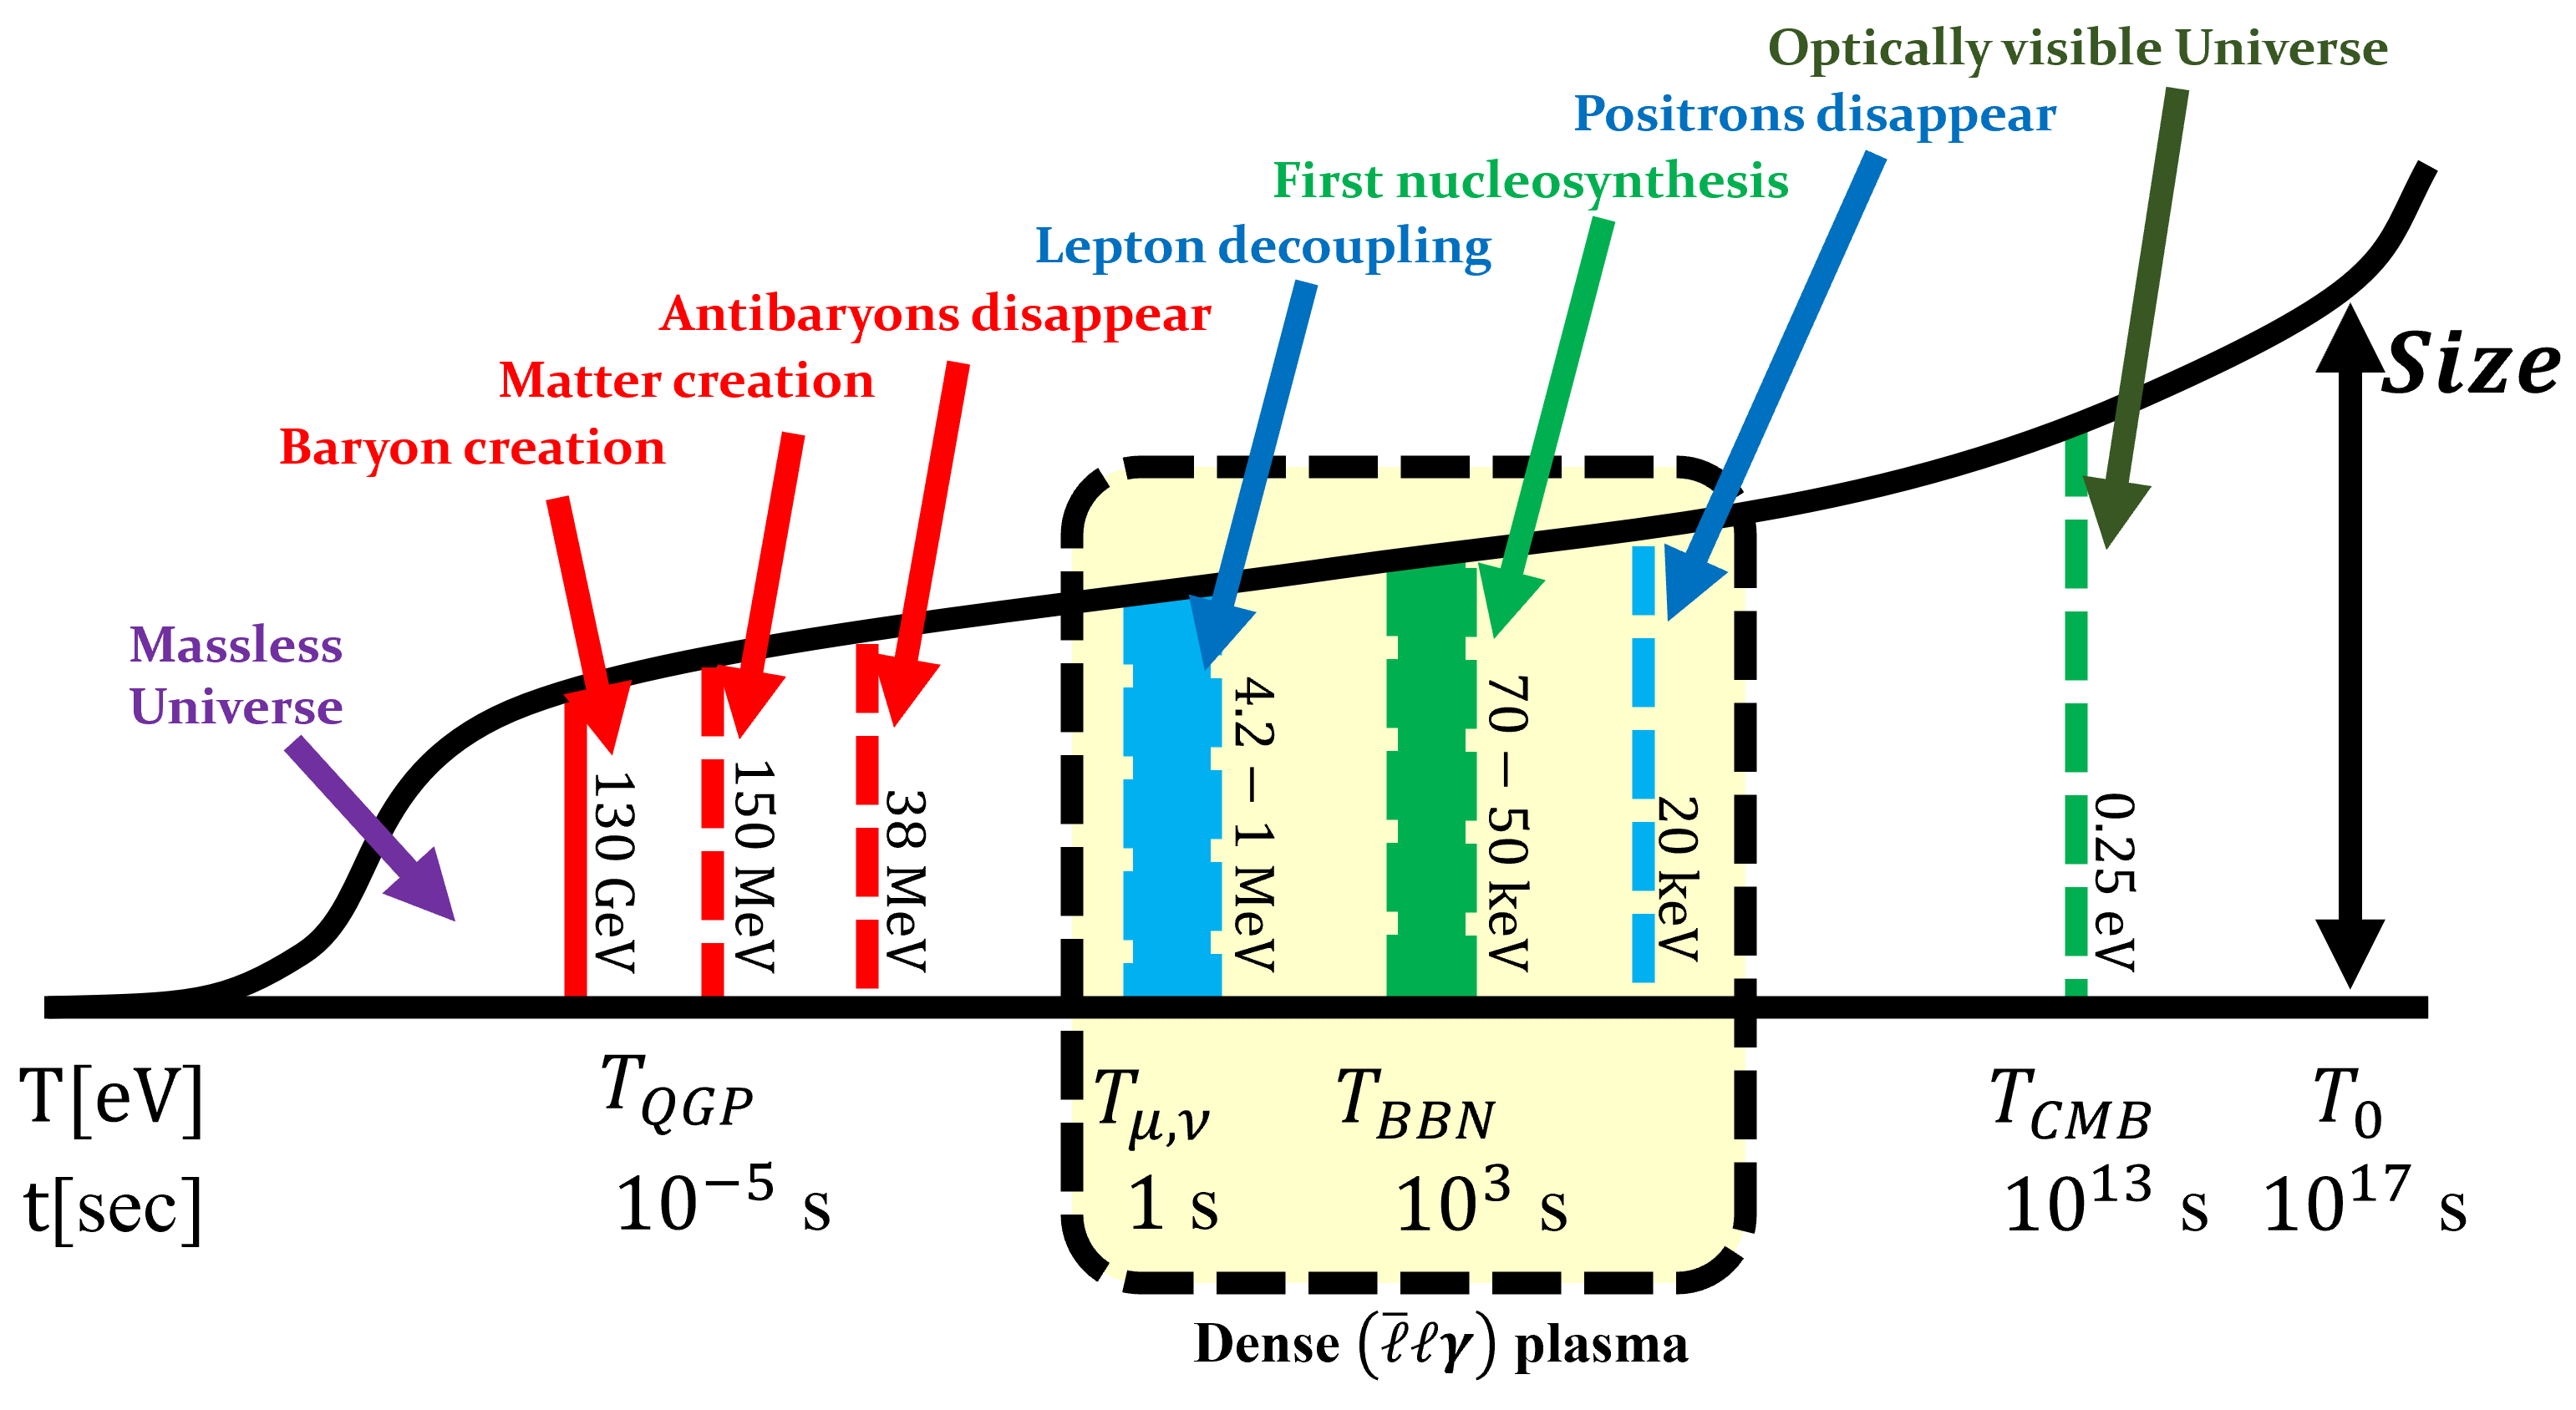
\includegraphics[width=0.95\linewidth]{plots/chap01intro/thesis_universe.png}
 \caption{A schematic of the universe's evolution since the Big Bang. The region of interest studied in this dissertation is emphasized (in the highlighted box) to contain a dense nearly charge neutral matter-antimatter plasma.}
 \label{fig:cosmo} 
\end{figure}
%%%%%%%%%%%%%%%%%%%%%%%%%%%%%%%%%%%%%%%

The scale factor $a(t)$ denotes the change of proper distances $L(t)$ over time as
\begin{gather}
    L(t)=L_{0}\frac{a_{0}}{a(t)}\rightarrow L(z)=L_{0}(1+z)\,,
\end{gather}
where $z$ is the redshift and $L_{0}$ the comoving length. In an expanding (or contracting) universe which is both homogeneous and isotropic, this implies volumes change with $V(t)=V_{0}/a^{3}(t)$ where $V_{0}=L_{0}^{3}$ is the comoving Cartesian volume. The evolutionary expansion of the universe is then traditionally defined in terms of the Hubble parameter $H(t)$ following the conventions in~\cite{weinberg1972gravitation}
\begin{gather}
  \label{Friedmann:1} H(t)^{2}\equiv\left(\frac{\dot a}{a}\right)^2=\frac{8\pi G_{N}}{3}\rho_\mathrm{total},\qquad \rho_\mathrm{total}(t)=\rho_{\Lambda}+\rho_\mathrm{DM}(t)+\rho_\mathrm{Baryons}(t)+\ldots\\
  \label{Friedmann:2}
  \frac{\ddot a}{a}=-qH^2,\qquad 
q\equiv -\frac{a\ddot a}{\dot a^2},\qquad \dot H=-H^2(1+q).
\end{gather}
where $G_N$ is the Newtonian constant of gravitation. \req{Friedmann:1} and \req{Friedmann:2} are also known as the Friedmann equations. The total density $\rho_\mathrm{total}$ is the sum of all contributions from any form of matter, radiation or field. This includes but is not limited to: dark energy $(\Lambda)$, dark matter (DM), baryons (B), leptons $(\ell,\nu)$ and photons $(\gamma)$. Depending on the age of the universe, the relative importance of each group changes as each dilutes different under expansion with dark energy infamously remaining constant in density and accelerating the universe today.

The parameter $q$ is the cosmic deceleration parameter where for historical reasons expansion is slowing down for $q>0$. before the discovery of dark energy. The early universe was radiation dominated with $q = 1$, subsequently matter dominated with $q = 1/2$, and the contemporary universe is undergoing a transition from matter to dark energy dominated whereas the deceleration settles on the asymptotic value of $q = -1$; see~\cite{Rafelski:2013yka}.

We can consider the expansion to be an adiabatic process~\citep{Abdalla:2022yfr} which results in a smooth shifting of the relevant dynamical quantities. As the universe undergoes isotropic expansion, the temperature decreases as 
\begin{gather}
 \label{tscale}
 T(t)=T_{0}\frac{a_{0}}{a(t)}\rightarrow T(z)=T_{0}(1+z)\,,
\end{gather}
where $z$ is the redshift. The entropy within a comoving volume is kept constant until gravitational collapse effects become relevant. The comoving temperature $T_{0}$ is given by the the present CMB temperature $T_{0}=2.7{\rm\ K}\simeq2.3\times10^{-4}\eV$~\citep{Planck:2018vyg}, with contemporary scale factor $a_{0}=1$.

As the universe expands, redshift reduces the momenta of particles lowering their contribution to the energy content of the universe. This cosmic redshift is written as
\begin{alignat}{1}
  \label{Redshift} p_{i}(t) = p_{i,0}\frac{a_{0}}{a(t)}\,.
\end{alignat}
Momentum (and the energy of massless particles $E=pc$) scales with the same factor as temperature. The energy of massive free particles in the universe however scales differently based on their momentum (and thus temperature).

When hot and relativistic, particle energy scales inversely like radiation. As the particles transition to non-relativistic (NR) momenta, their energies scale with the inverse square of the scale factor
\begin{alignat}{1}
    \label{EScale} E(t) = E_{0}\frac{a_{0}}{a(t)}\xrightarrow{\mathrm{NR}}\  E_{0}\frac{a_{0}^{2}}{a(t)^{2}}\,.
\end{alignat}
This occurs because of the functional dependence of energy on momentum in the relativistic $E\sim p$ versus non-relativistic $E\sim p^{2}$ cases.
% Chapter 2 - Magnetic dipoles
%%%%%%%%%%%%%%%%%%%%%%%%%%%%%%%%%%%%%%%
\chapter{Dynamics of charged particles with arbitrary magnetic moment}
\label{chap:moment}
%%%%%%%%%%%%%%%%%%%%%%%%%%%%%%%%%%%%%%%
\noindent This chapter reviews our work done in exploring relativistic dynamics with arbitrary magnetic dipoles in both a quantum mechanical and classical context. \rsec{sec:kgpapplications} is primarily based on~\cite{Steinmetz:2018ryf} and covers analytic solutions for the Klein-Gordon-Pauli (KGP) equation in the presence of homogeneous magnetic fields (\rsec{sec:homogeneous}) and the Coulomb problem (\rsec{sec:coulomb}) for hydrogen-like atoms. Comparisons with the Dirac-Pauli (DP) and Dirac solutions are made and novel consequences for strong fields are discussed.

\rsec{sec:kgptopics} covers special topics related to KGP including a proposal which couples mass and magnetic moment (\rsec{sec:ikgp}) and an extension to particles (such as quarks) which are charged under both Albelian and non-Albelian fields (\rsec{sec:quarks}). The second special topic is yet unpublished outside this dissertation.

Relativistic classical spin dynamics is discussed in \rsec{sec:cspin} and is based on our work in~\cite{Rafelski:2017hce}. We propose in \rsec{sec:magpotential} a covariant form of magnetic dipole potential which modifies the Lorentz force, extends the Thomas-Bargmann-Michel-Telegdi (TMBT) equation, and reproduces the Stern-Gerlach force in the non-relativistic limit. \rsec{sec:ampgil} discusses our finding that this magnetic potential also serves to unify both the Amp{\`e}rian and Gilbertian pictures of dipole moments.

%%%%%%%%%%%%%%%%%%%%%%%%%%%%%%%%%%%%%%%
\section{Analytic solutions of the Klein-Gordon-Pauli}
\label{sec:kgpapplications}
%%%%%%%%%%%%%%%%%%%%%%%%%%%%%%%%%%%%%%%
\noindent In \rsec{sec:mom}, we addressed two different models of introducing anomalous magnetic moment in QM: 
\begin{enumerate}%[label=(\alph*)]
\item[(a)] the Dirac-Pauli (DP) first order equation which is the Dirac equation where $g$-factor is precisely fixed to the $g\!=\!2$, with the addition of an incremental Pauli term; and
\item[(b)] the Klein-Gordon-Pauli (KGP) second order equation which \lq\lq squares\rq\rq\ the Dirac equation and thereafter allows the magnetic moment $\bb{\mu}$ to vary independently of charge and mass, unlike Dirac theory.
\end{enumerate} 
These two approaches coincide when the anomaly $a$ vanishes. However, all particles that have magnetic moments differ from the Dirac value $g\!=\!2$, either due to their composite nature, or, for point particles, due to the quantum vacuum fluctuation effect.

We find in this chapter that even a small magnetic anomaly has a large effect in the limit of strong fields generated by massive magnetar stars~\citep{Kaspi:2017fwg}. Therefore it is not clear that the tacit assumption of $g\!=\!2$ in the case of strong fields~\citep{Rafelski:1976ts,Greiner:1985ce,Rafelski:2016ixr} is prudent~\citep{Evans:2018kor}. This argument is especially applicable to tightly bound composite particles such as protons and neutrons where the large anomalous magnetic moment can be taken as an external prescribed parameter unrelated to the elementary quantum vacuum fluctuations. It is then of particular interest to study the dynamical behavior of these particles in fields of magnetar strength. This interest carries over to the environment of strong fields created in focus of ultra-intense laser pulses and the associated particle production processes~\citep{Dunne:2014qda,Hegelich:2014tda}. We consider also precision spectroscopic experiments and recognize consequences even in the weak coupling limit.

%%%%%%%%%%%%%%%%%%%%%%%%%%%%%%%%%%%%%%%
\subsection{Homogeneous magnetic fields}
\label{sec:homogeneous}
%%%%%%%%%%%%%%%%%%%%%%%%%%%%%%%%%%%%%%%
\noindent The case of the homogeneous magnetic field, sometimes referred to as the Landau problem, provides a stepping stone in which to examine all other consequences of quantum spin dynamics. A full treatment of this solution in terms of Ladder operators can be found in~\cite{Steinmetz:2018ryf} while alternative approaches are shown in texts such as~\cite{Itzykson:1980rh}. We take a constant magnetic field in the $z$-direction to be
\begin{alignat}{1}
	\label{homogeneous:1} \bb{B}=(0,0,B)\,.
\end{alignat}
For our choice of gauge, there are two common options: (a) the Landau $\bb{A}_\mathrm{L}$ gauge and (b) the symmetric $\bb{A}_\mathrm{S}$ gauge
\begin{alignat}{1}
	\label{homogeneous:2} \bb{A}_\mathrm{L}=B(0,x,0)\,,\indent \bb{A}_\mathrm{S}=\frac{B}{2}(-y,x,0)\,.
\end{alignat}
As the system has a manifest rotational symmetry perpendicular to the direction of the homogeneous field, we will choose the symmetric gauge $\bb{A}_\mathrm{S}$ which preserves this symmetry explicitly.

Before we examine relativistic wave equations, it will be helpful to first consider the non-relativistic Schr{\"o}dinger-Pauli case as the KGP-Landau problem can be written as equivalent to the Schro{\"o}dinger-Pauli Hamiltonian. We consider energy eigenstates of \req{sp:1} under \req{homogeneous:1} as
\begin{alignat}{1}
	\label{homogeneous:3} \chi\rightarrow\chi_\mathrm{E}\exp\left(-\frac{iEt}{\hbar}\right)\,,\qquad\left(\frac{1}{2m_{\ell}}\bb{\pi}^{2}-\bb{\mu}\cdot\bb{B}\right)\chi_\mathrm{E}=E\chi_\mathrm{E}\,,
\end{alignat}
where $\mu$ is the magnitude of the magnetic moment as defined in \req{mag:3}. \req{homogeneous:3} can be further rewritten using angular momentum $\bb{L}$ and the symmetric gauge \req{homogeneous:2} as
\begin{gather}
	\label{homogeneous:4} \left(\frac{1}{2m_{\ell}}\bb{p}^{2}+\frac{e^{2}B^{2}}{8m_{\ell}}(x^{2}+y^{2})-\frac{eB}{2m_{\ell}}L_{3}-\mu B\sigma_{3}\right)\chi_\mathrm{E}=E\chi_\mathrm{E}\,,\\
    \bb{L}=\bb{r}\times\bb{p}\,,\qquad L_{i}=\varepsilon_{ijk}x_{j}p_{k}\,.
\end{gather}

The above can be broken into a set of three mutually commuting Hamiltonian operators: (a) the free particle Hamiltonian, (b) the quantum harmonic oscillator (HO), and (c) the Zeeman interaction (ZI) given by
\begin{align}
	\label{homogeneous:7}
    &H_\mathrm{total}=H_\mathrm{Free}+H_\mathrm{HO}+H_\mathrm{Mag.}\,,\\
	\label{homogeneous:7a}
    &H_{\mathrm{Free}}=\frac{p_{3}^{2}}{2m}\,,\\
	\label{homogeneous:7b}
    &H_\mathrm{HO}\,=\frac{1}{2m_{\ell}}\left(p_{1}^{2}+p_{2}^{2}\right) + \frac{1}{2}m_{\ell}\omega^{2}(x^{2}+y^{2})\,,\\
	\label{homogeneous:7c}
    &H_{\mathrm{ZI}}\ \,=-\mu_{\ell}B\frac{L_{3}}{\hbar}-\mu B\sigma_{3}\,.
\end{align}
The cyclotron frequency appears in \req{homogeneous:7b} as $2\omega=\omega_\mathrm{C}=eB/m_{\ell}$. We note that the \req{homogeneous:7c} is usually expressed as
\begin{alignat}{1}
	\label{homogeneous:7d}
    H_{\mathrm{ZI}}=-\frac{e}{2m}\left(\bb{L}+g\bb{S}\right)\cdot\bb{B}\,,
\end{alignat}
with $\bb{S}$ defined in \req{qspin:1}. We see more explicitly that the orbital gyromagnetic ratio $g_\mathrm{L}$ which is a coefficient to the angular momentum operator $\bb{L}$ is unity unlike for spin. As all the above Hamiltonian operators are mutually commuting, the energy eigenvalue of the total Hamiltonian is the sum of the individual energy eigenvalues. Our remaining goal will be to convert the KGP eigenvalue equation into the above three non-relativistic Hamiltonian operators. 

We now return to the KGP equation and write expand \req{kgp:1} for the Landau problem with energy eigenstates $\Psi_\mathrm{E}$ yielding
\begin{alignat}{1}
    \label{lan09}
    \left(\frac{E^{2}}{c^{2}}-m^{2}c^{2}-\bb{p}^{2}-\frac{1}{4}e^{2}B^{2}\left(x^{2}+y^{2}\right)+eBL_{3}+2\mu m_{\ell} B\sigma_{3}\right)\Psi_\mathrm{E}=0\;.
\end{alignat} 
We introduce the substitutions 
\begin{alignat}{1}
    \label{lan10}
    E\to m^\prime c^{2}\,,\quad \frac{E^{2}-m_{\ell}^{2}c^{4}}{2E}\to E^\prime\;,
\end{alignat} 
and arrive at the Schr{\"o}dinger-style Hamiltonian equation
\begin{gather}
	\label{lan11} \left(\frac{1}{2m'}\bb{p}^{2}+\frac{e^{2}B^{2}}{8m'}(x^{2}+y^{2})-\frac{eB}{2m'}L_{3}-\mu\left(\frac{m_{\ell}}{m'}\right)B\sigma_{3}\right)\Psi_\mathrm{E}=E'\Psi_\mathrm{E}\,,
\end{gather}
which matches the non-relativistic Hamiltonian presented in \req{homogeneous:7}.

After a lengthy derivation (see~\cite{Steinmetz:2018ryf}), the energy eigenvalues are given by
\begin{alignat}{1}
    \label{lan23}
    E'&=\frac{p_{3}^{2}}{2m^\prime }+\frac{e\hbar B}{m^\prime}\left(n+\frac{1}{2}\right)-\mu\left(\frac{m_{\ell}}{m'}\right)Bs\,,
\end{alignat}
where $n\in1,2,3\ldots$ is the Landau orbital quantum number and $s\in\pm1$ is the spin quantum number.









%%%%%%%%%%%%%%%%%%%%%%%%%%%%%
\subsubsection*{Dirac and KGP Case}\label{ajsss:DKGP}
\noindent As mentioned in \rsec{ajsss:homogeneous}, the non-relativistic Pauli system and the Dirac and KGP systems are mathematically equivalent for homogeneous fields. This allows us to pull the relativistic energy $E_{R}$ eigenvalues straight from the non-relativistic $E_{NR}$ values via the substitution and redefinition of non-relativistic mass $m_{NR}$
\begin{alignat}{1}
	\label{eq:DKGP:01} E_{NR} = \frac{E_{R}^{2}-m_{R}^{2}c^{4}}{2E_{R}}\,,\indent  E_{R} = m_{NR}c^{2}\,.
\end{alignat}
The resulting eigenvalues, dropping the relativistic subscripts, are then given by
\begin{alignat}{1}
	\label{eq:DKGP:02} E_{KGP} =\pm\sqrt{m^{2}c^{4}+p_{z}^{2}c^{2}+2e\hbar c^{2}B\left(n+\frac{1}{2}\right)\pm2\mu mc^{2}B}\,.
\end{alignat}
To obtain the Dirac levels, simply set $g\!=\!2$. In this equation, we can clearly see the energy contribution contains an orbital part, which houses the transverse $x$ and $y$-momentum, and a magnetic contribution which can either raise of lower the level. In the Dirac case, there is a degeneracy among Landau levels as in the non-relativistic case which is then broken by the presence of the anomaly.

%%%%%%%%%%%%%%%%%%%%%%%%%%%%%%%%%%%%%%%
\subsection{Hydrogen-like atoms}
\label{sec:coulomb}
%%%%%%%%%%%%%%%%%%%%%%%%%%%%%
The Coulomb problem, or sometimes referred to as the Kepler problem, provides us with a standard application of any quantum theory to explore. As the hydrogen-like atom is the most well understood atomic system in physics, any non-minimal behavior especially for high-$Z$ systems can lead to dramatic consequences for the resulting spectra. We take the Coulomb potential to be
\begin{equation}
	\label{eq:coulomb:01} V_\mathrm{C}\equiv e A^{0}=\frac{Z \alpha\hbar c}{r}\;,\qquad \vec{A}=\vec{0}\;.
\end{equation}
The KGP-Coulomb problem can be solved analytically \ar We will briefly sketch out the solution and its consequences. For energy states $\Psi=e^{-iEt/\hbar}\psi_\mathrm{E}$ the KGP equation yields the following differential equation
\begin{alignat}{1}
	\label{cou02} \left(\frac{E^{2}-m^{2}c^{4}}{\hbar^{2}c^{2}}+\frac{Z^{2}\alpha^{2}}{r^{2}}+\frac{2E}{\hbar c}\frac{Z\alpha}{r}+\frac{1}{r}\frac{\partial^{2}}{\partial r^{2}}r-\frac{L^{2}/\hbar^{2}}{r^{2}}-\frac{g}{2}Z\alpha\frac{i\vec{\alpha}\cdot\hat{r}}{r^{2}}\right)\psi_\mathrm{E}=0\;.
\end{alignat}
We recast the squared angular momentum operator $L^{2}$ with the Dirac spin-alignment operator
\begin{alignat}{1}
\label{cou04} &\mathcal{K}=\gamma^{0}\left(1+\bb{\Sigma}\cdot\frac{\bb{L}}{\hbar}\right)\;,\indent L^{2}/\hbar^{2}=\mathcal{K}\left(\mathcal{K}-\gamma^{0}\right)\;.
\end{alignat}
The operator $\mathcal{K}$ commutes with $\vec{\alpha}\cdot\hat{r}$ and its eigenvalues are given as either positive or negative integers $\kappa=\pm(j+1/2)$ where $j$ is the total angular momentum quantum number. By grouping all terms proportional to $1/r^{2}$, we see the effective angular momentum eigenvalues take on non-integer values which in the limit of classical mechanics corresponds to orbits which do not close. \ar The non-integer eigenvalues depends explicitly on $g$-factor. The difficulty of this equation is that the effective angular momentum operator is non-diagonal in spinor space due to the presence of $\vec{\alpha}\cdot\hat{r}$ which mixes upper and lower components. The effective radial potential within \req{cou02} is then
\begin{alignat}{1}
	\label{temp} V_\mathrm{eff}=-\frac{2E}{\hbar c}\frac{Z\alpha}{r}
\end{alignat}
Following the procedure of Martin and Glauber~\cite{Martin:1958zz}, we introduce the operator
\begin{alignat}{1}
\label{cou07} &\mathfrak{L}=-\gamma^{0}\mathcal{K}-\frac{g}{2}Z\alpha(i\vec{\alpha}\cdot\hat{r})\;,
\end{alignat}
but with the novel modification that $g$-factor directly appears in the second term. This operator is also sometimes referred to as the Temple operator. This then commutes with the spin-alignment operator $\mathcal{K}$ and has eigenvalues
\begin{alignat}{1}
\label{cou08} &\Lambda=\pm\sqrt{\kappa^{2}-\displaystyle\frac{\displaystyle g^{2}}{4}Z^{2}\alpha^{2}}\;,\end{alignat}
where the absolute values are denoted as $\lambda=|\Lambda|$. The numerator of the last term in \req{cou06} can be then replaced by
\begin{alignat}{1}
\label{cou09} &\mathcal{K}(\mathcal{K}-\gamma^{0})-Z^{2}\alpha^{2}-\frac{g}{2}Z\alpha(i\vec{\alpha}\cdot\hat{r})=\mathfrak{L}(\mathfrak{L}+1)+\left(\frac{g^{2}}{4}-1\right)Z^{2}\alpha^{2}.
\end{alignat}
If the $g$-factor is taken to be $g\!=\!2$, then the differential \req{cou06} reverts to the one discussed in Martin and Glauber\rq s work~\cite{Martin:1958zz}. The coefficient $g^{2}/4-1$ will be commonly seen to precede new more complicated terms, which conveniently vanish for $|g|=2$ demonstrating that as function of $g$ there is a \lq\lq cusp\rq\rq~\cite{Rafelski:2022bsv} for $|g|=2$. This will become especially evident when we discuss strongly bound systems in section~\ref{sb}, which behave very differently for $|g|<2$ versus $|g|>2$. 

The energy levels of the KGP-Coulomb equation are then
\begin{subequations}
\begin{alignat}{1}
\label{cou17} E_{\pm\lambda}^{n_{r},j}&=\frac{mc^{2}}{\sqrt{1+\displaystyle\frac{Z^{2}\alpha^{2}}{\left(n_{r}+\frac{1}{2}+\sqrt{(\lambda\pm1/2)^{2}+\left(\frac{g^{2}}{4}-1\right)Z^{2}\alpha^{2}}\right)^{2}}}},\\[0.2cm]
\label{cou17c} \lambda&=\sqrt{\displaystyle(j+1/2)^{2}-\frac{\displaystyle g^{2}}{4}Z^{2}\alpha^{2}}\;.
\end{alignat}
\end{subequations}
\req{cou17} is the same \lq\lq Sommerfeld-style\rq\rq\ expression for energy that we can obtain from the Dirac or KG equations. The difference between them arises from the expression of the relativistic angular momentum which depends on $g$-factor for the KGP equation. The KGP eigenvalues \req{cou17} were also obtained by Niederle and Nikitin~\cite{Niederle:2004bx} using a tensor-spinorial approach for arbitrary half-integer spin particles.

Because we are treating $g$-factor as a unbounded parameter we need to verify that the Dirac and Klein-Gordon energy spectra, which can be found in most texts, see for example Itzykson and Zuber~\cite{Itzykson:1980rh}, emerges from the appropriate limit of $g$-factor. In the limit that $g\rightarrow2$ for the Dirac case the expressions for $\lambda$ and $\nu$ reduce to
\begin{subequations}
\begin{alignat}{1}
\label{glimit01} &\lim_{g\rightarrow2}\lambda=\sqrt{\displaystyle(j+1/2)^{2}-Z^{2}\alpha^{2}},\\
&\lim_{g\rightarrow2}\nu_{\pm\lambda}=\lambda\pm1/2\;.
\end{alignat}
\end{subequations}
This procedure requires taking the root of perfect squares; therefore, the sign information is lost in \req{glimit01}. As long as $Z^{2}\alpha^{2}<3/4$ we can drop the absolute value notation as $\nu$ is always positive. The energy is then given by
\begin{alignat}{1}
\label{glimit02} &E_{\pm\lambda}^{n_{r},j}=\frac{mc^{2}}{\sqrt{1+\displaystyle\frac{Z^{2}\alpha^{2}}{\left(n_{r}\begin{smallmatrix} +1 \\ +0 \end{smallmatrix}+\sqrt{\displaystyle(j+1/2)^{2}-Z^{2}\alpha^{2}}\right)^{2}}}}\;.
\end{alignat}
The $\begin{smallmatrix} +1 \\ +0 \end{smallmatrix}$ notation is read as the upper value corresponding to the $+\lambda$ states and the lower value corresponding to the $-\lambda$ states. 

The ground state energy (with: $n_{r}=0,\ \Lambda<0,\ j=1/2$) is therefore
\begin{alignat}{1}
\label{glimit07} &E^{0,1/2}_{-\lambda(j=1/2)}=mc^{2}\sqrt{1-Z^{2}\alpha^{2}}\;,\end{alignat}
as expected for the Dirac-Coulomb ground state. \req{glimit02} reproduces the Dirac-Coulomb energies and also contains a degeneracy between states of opposite $\lambda$ sign, same $j$ quantum number and node quantum numbers offset by one
\begin{alignat}{1}
\label{glimit03} &E^{n_{r}+1,j}_{-\lambda}=E^{n_{r},j}_{+\lambda}\;,\end{alignat}
which will see in section~\ref{nonrel} corresponds to the degeneracy between $2S_{1/2}$ and $2P_{1/2}$ states. There is no degeneracy for the $E^{0,j}_{-\lambda}$ states. 

In the limit that $g\rightarrow 0$, which is the KG case, the expressions are given by
\begin{subequations}
\begin{alignat}{1}
\label{glimit04} &\lim_{g\rightarrow0}\lambda=j+1/2,\\
&\lim_{g\rightarrow0}\nu_{\pm\lambda}=\sqrt{\left(j\begin{smallmatrix} +1 \\ +0 \end{smallmatrix}\right)^{2}-Z^{2}\alpha^{2}}\;,
\end{alignat}
\end{subequations}
which reproduces the correct expressions for the energy levels for the Klein-Gordon case 
\begin{alignat}{1}
\label{glimit05} &E_{\pm\lambda}^{n_{r},j}=\frac{mc^{2}}{\sqrt{1+\displaystyle\frac{Z^{2}\alpha^{2}}{\left(n_{r}+1/2+\displaystyle\sqrt{\left(j\begin{smallmatrix} +1 \\ +0 \end{smallmatrix}\right)^{2}-Z^{2}\alpha^{2}}\right)^{2}}}}\;,\end{alignat}
except that in this limit we are still considering the total angular moment quantum number $j$ rather than orbital momentum quantum number $\ell$. It is interesting to note that the KG-Coulomb problem\rq s energy formula contains $\ell+1/2$, which matches identically to our half-integer $j$ values; therefore, this artifact of spin, untethered and invisible by the lack of magnetic moment, does not alter the energies of the states. The degeneracy in energy levels are given by 
\begin{alignat}{1}
\label{glimit06} &E^{n_{r},j+1}_{-\lambda}=E^{n_{r},j}_{+\lambda}\;,\end{alignat}
with levels of opposite $\lambda$ sign, same node quantum number and shifted $j$ values by one. In a similar fashion to the Dirac case, here we have no degeneracy for $E^{n_{r},1/2}_{-\lambda}$ states. In section~\ref{nonrel} we will convert from $n_{r}$, $j$ and $\pm\lambda$ to the familiar quantum numbers of $n$, $j$ and $\ell$ allowing for easy comparison with the hydrogen spectrum in standard notation.

%%%%%%%%%%%%%%%%%%%%%%%%%%%%%%%%%%%%%%%
\subsubsection{Critical field strengths}
\noindent The magnetic moment anomaly can lead to interesting behaviors in the strong EM field systems. The anomaly can flip the sign of the magnetic energy for the least excited states causing the gap between particle and antiparticle states to decrease with magnetic field strength. By setting the longitudinal momentum $p_{z}$ to zero, we can see that the energy of the lowest KGP Landau eigenstate $n=0,\ s=1/2$ reaches zero where the gap between particle and antiparticle states vanishes for the field
\begin{subequations}
\begin{alignat}{1}\label{Bcrit}
&B_\mathrm{crit}^{e}=\frac{\mathcal{B}_\mathrm{S}^{e}}{a_{e}}=861\mathcal{B}_\mathrm{S}^{e} =3.8006\times10^{12}\;\mathrm{T}\;,\\
&B_\mathrm{crit}^{p}=\frac{\mathcal{B}_\mathrm{S}^{p}}{a_{p}}=\frac{1}{1.79}\mathcal{B}_\mathrm{S}^{p}=8.3138\times10^{15}\;\mathrm{T}\;,
\end{alignat} 
\end{subequations}
where $\mathcal{B}_\mathrm{S}$ is the Schwinger critical field~\cite{Schwinger:1951nm}.
\begin{subequations}
\begin{alignat}{1}\label{Bsch}
\mathcal{B}_\mathrm{S}^{e}\equiv\frac{{m_{e}^2}c^3}{e\hbar}=\frac{m_{e}c^2}{2\mu_B}=4.4141\times 10^{9}\;\mathrm{T}\;,\\
\mathcal{B}_\mathrm{S}^{p}\equiv\frac{{m_{p}^2}c^3}{e\hbar}=\frac{m_{p}c^2}{2\mu_N}=1.4882\times 10^{16}\;\mathrm{T}\;.
\end{alignat}
\end{subequations}
The numerical results are evaluated for the anomalous moment of the electron and proton, given by \req{aeFULL} and \req{gpaFULL}. At the critical field strength $B_\mathrm{crit}$ the Hamiltonian loses self-adjointness and the KGP loses its predictive properties. The Schwinger critical field \req{Bsch} denotes the boundary when electrodynamics is expected to behave in an intrinsically nonlinear fashion, and the equivalent electric field configurations become unstable~\cite{Labun:2008re}. However, it is also possible that the vacuum is stabilized by such strong magnetic fields~\cite{Evans:2018kor}.

The critical magnetic fields as shown in \req{Bcrit} appear in discussion of magnetars~\cite{Kaspi:2017fwg}. The magnetar field is expected to be more than 100-fold that of the Schwinger critical magnetic field which is on the same order of magnitude as $B_\textrm{crit}$ for an electron. While the critical field for a proton exceeds that of a magnetar, the dynamics of protons (and neutrons) in such fields is nevertheless significantly modified. A correct description of magnetic moment therefore has relevant consequences to astrophysics. 

Figure~\ref{f02} shows analogous reduction in particle/anti\-particle energy gap for the DP equation. In this case the vanishing point happens at a larger magnetic field strength. This time the solutions continue past this point, but require allowing the states to cross into the opposite continua which we consider unphysical. We are not satisfied with either model\rq s behavior though the KGP description is preferable for reasons stated earlier in section~\ref{lan}. However, it is undesirable that both KGP and DP solutions loose physical meaning and vacuum stability in strong magnetic fields.

%%%%%%%%%%%%%%%%%%%%%%%%%%%%%%%%%%%%%%%
\subsubsection{Applicability of DP or KGP to critical fields}\label{vacfl}
Care must be taken when interpreting the results presented in section~\ref{lan}. For physical electrons the AMM interaction is the result of vacuum fluctuations whose strength also depends on the strength of the field. For example in the large magnetic field limit a QED computation shows that the ground state is instead of \req{lan25b} given by~\cite{Jancovici:1969exc}
\begin{alignat}{1} \label{vacfl01}
E_{0}\approx mc^{2}+\frac{\alpha}{4\pi}mc^{2}\ \mathrm{ln}^{2}\left(\frac{2e\hbar B}{m^{2}c^{3}}\right)
\end{alignat}
which even for enormous magnetic fields does not deviate significantly from the rest mass-energy of the electron. Further the AMM  radiative corrections approach zero for higher Landau levels~\cite{Ferrer:2015wca}. Therefore the AMM in the case of electrons does not have a significant effect in highly magnetized environments such as those found in astrophysics (magnetars).

The situation is different for composite particles such as the proton, neutron and light nuclei whose anomalous magnetic moments are dominated by their internal structure and not by vacuum fluctuations. In this situation we expect that the AMM interaction in high magnetic fields remains significant. Therefore, asking whether the DP or KGP equations better describes the dynamics of composite hadrons and atomic nuclei in presence of magnetar strength fields is a relevant question despite the standard choice in literature being the DP equation~\cite{Broderick:2000pe}. The same question can be asked for certain exotic hydrogen-like atoms where the constituent particles have anomalous moments which can be characterized as an external parameter. 

%%%%%%%%%%%%%%%%%%%%%%%%%%%%%%%%%%%%%%%
\section{Topics related to Klein-Gordon-Pauli}
\label{sec:kgptopics}
%%%%%%%%%%%%%%%%%%%%%%%%%%%%%%%%%%%%%%%
\subsection{Unification of mass and magnetic moment}
\label{sec:ikgp}
%%%%%%%%%%%%%%%%%%%%%%%%%%%%%%%%%%%%%%%
While we've thus far focused on the Dirac-Pauli and Klein-Gordon-Pauli models for magnetic dipole moments, the non-uniqueness of spin dynamics allows us to invent further non-linear EM models which all in the non-relativistic limit yield the non-relativisitc QM magnetic dipole Hamiltonian. One such extension to quantum spin dynamics is to note the close relationship mass and magnetic moment share in the KGP formalism. We can write a unified dipole-mass as
\begin{alignat}{1}
    \label{eq:ext:01} \widetilde{m}c^{2}=mc^{2}+\frac{i}{2}\mu\left(\gamma_{\alpha}\partial^{\alpha}\gamma_{\beta}A^{\beta}\right)\,,
\end{alignat}
which satisfies the wave equation
\begin{alignat}{1}
    \label{eq:ext:02} \left((i\hbar c\partial-eA)^{2}-(\widetilde{m}c^{2})^{2}\right)\Psi=0\,.
\end{alignat}
This modified KGP formulation then requires spin sensitive mass and an explicit electromagnetic component to the charged lepton mass. As informed by classical mechanics, charged particles should be understood to derive at least some of their mass from the mass-energy of their electromagnetic fields. While the classical model fails because it yields an infinite electromagnetic mass, the underlying argument should still be true though some mechanism must ensure that the mass-energy of the electric field is finite. A classical example is the electromagnetic mass of the charged black hole which is finite. This still remains an open problem in physics. This approach in \req{eq:ext:01} is superficially similar to the of the Frenkel model in classical mechanics by giving the particle a spin dependent mass, but this formulation is distinct in that the mass here is allowed off-diagonal components in spinor space. The dipole-mass is off-diagonal in spinor space in the Dirac representation and no longer commutes likes a scalar. \req{eq:ext:02} differs from the regular KGP equation by the presence of an additional interaction term
\begin{alignat}{1}
    \label{eq:ext:03} \delta V=-\frac{\mu^{2}}{4}\left(\gamma_{\alpha}\partial^{\alpha}\gamma_{\beta}A^{\beta}\right)^{2}\,.
\end{alignat}
\req{eq:ext:03} results in higher order vertex diagrams coupling fermions to photons. Taking advantage of the invariants of the electromagnetic field tensor $F^{\mu\nu}$ we can rewrite \req{eq:ext:03} as
\begin{alignat}{1}
    \label{eq:ext:04a} \delta V=-2\mu^{2}\left(\mathcal{S}+i\gamma^{5}\mathcal{P}\right)\,,\indent\mathcal{S}=\frac{1}{2}(\bb{B}^{2}-\bb{E}^{2})\,,\indent \mathcal{P}=\bb{E}\cdot\bb{B}\,.
\end{alignat}
This represents simply only one possible non-linear extension to electromagnetism in relativistic quantum mechanics of which there are a family of extensions~\citep{Foldy:1952a}.

%%%%%%%%%%%%%%%%%%%%%%%%%%%%%%%%%%%%%%%
\subsection{Extensions to non-Albelian fields}
\label{sec:quarks}
%%%%%%%%%%%%%%%%%%%%%%%%%%%%%%%%%%%%%%%

While most attention in particle physics focusses on the dipole moments of fermions, it is well known that bosons with spin can also carry dipole moments. The most pertinant example is that of the W-boson which after electroweak symmetry breaking has a magnetic dipole term which is analogous to the Pauli term in KGP or DP for fermions. While a wide variety of spin-1 formulations exist, such as the Duffin-Kemmer formulation \ar, in the following discussion we will write in the Proca formulation as it is most similar to how electromagnetic fields, which are also spin-1 fields, are written. For a complex spin-1 field, the Proca action is given by
\begin{alignat}{1}
	\label{eq:proca:01a} \mathcal{L}_{\mathrm{Proca}} = -\frac{1}{2}\mathcal{F}_{\mu\nu}^{*}\mathcal{F}^{\mu\nu}+\frac{m^{2}c^{2}}{\hbar^{2}}B_{\mu}^{*}B^{\mu}\,,\\
	\label{eq:proca:01b} \mathcal{F}^{\mu\nu}=\partial^{\mu}B^{\nu}-\partial^{\nu}B^{\mu}\,.
\end{alignat}
The Euler-Lagrangian equations of motion are then
\begin{alignat}{1}
	\label{eq:proca:02a} \partial_{\mu}\mathcal{F}^{\mu\nu}+\frac{m^{2}c^{2}}{\hbar^{2}}B^{\nu}=0\,,
\end{alignat}
which if the Lorenz gauge $\partial\cdot B=0$ is taken simplifies to a Klein-Gordon style second-order wave equation. If we gauge the fields giving the spin-1 field an electric charge, we can produce a theory which naturally generates a magnetic moment.

Briefly, we would like to comment on the g-factor of the quarks who unlike the leptons also participate in the strong color interaction. Since color charge follows a more complex SU(3) group structure unlike the more straight forward U(1) of electromagnetism, the \lq\lq color magnetism\rq\rq\ of QCD requires more than just the analogous Pauli term to describe color dipole moments owing due to the fact that QCD has non-Abelian gauge fields. The quarks, like the leptons, should obey the quantum mechanical analogue of the energy-momentum relation seen in \req{eq:spin:03} with the only theoretical difference being a differing covariant derivative. The covariant derivative, written in terms of momentum, should appear as
\begin{alignat}{1}
	\label{eq:spin:08} \pi^{\alpha}=p^{\alpha}-g_\mathrm{S}\mathcal{A}^{\alpha}\,,
\end{alignat}
where $g_\mathrm{S}$ is the color charge strength and not to be confused with the QCD notion of g-factor. The gluon fields $\mathcal{A}^{\alpha}$ is a $3\times3$ matrix to accomodate the three charges of QCD: red, green and blue. The eight Gell-Mann $\lambda^{a}$ matrices are embbeded into the gluon field for each possible gluon charge.
\begin{alignat}{1}
	\label{eq:spin:09} \mathcal{A}^{\alpha}\equiv\frac{1}{2}\lambda^{a}\mathcal{A}^{\alpha}_\mathrm{A}\,,\indent a\in1\ldots8\,,
\end{alignat}
We note the non-commuting behavior of the Gell-Mann matrices which capture the non-Abelian structure of the gauge fields. The gluon strength tensor $\mathcal{G}^{\mu\nu}$ is then
\begin{alignat}{1}
	\label{eq:spin:10a} \mathcal{G}^{\mu\nu}\equiv\partial^{\mu}\mathcal{A}^{\nu}-\partial^{\nu}\mathcal{A}^{\mu}+ig_\mathrm{S}\left[\mathcal{A}^{\mu},\mathcal{A}^{\nu}\right]\,,\\
	\label{eq:spin:10b} \left[\mathcal{A}^{\mu},\mathcal{A}^{\nu}\right] = \frac{1}{4}\mathcal{A}^{\mu}_\mathrm{A}\mathcal{A}^{\nu}_{b}\left[\lambda^{a},\lambda^{b}\right]=\frac{i}{2}\mathcal{A}^{\mu}_\mathrm{A}\mathcal{A}^{\nu}_{b}f^{abc}\lambda_{c}\,,
\end{alignat}
where $f^{abc}$ are the structure constants of the SU(3) group. The resulting KGP equation for color charge with $g\!=\!2$ then appears as
\begin{alignat}{1}
	\label{eq:spin:11} \left(\eta_{\alpha\beta}\pi^{\alpha}\pi^{\beta}-\frac{g_\mathrm{S}\hbar}{2}\sigma_{\alpha\beta}\left(\partial^{\mu}\mathcal{A}^{\nu}-\partial^{\nu}\mathcal{A}^{\mu}+ig_\mathrm{S}\left[\mathcal{A}^{\mu},\mathcal{A}^{\nu}\right]\right)\right)\Psi&=m^{2}c^{2}\Psi\,,
\end{alignat}
which mirrors the electromagnetic case except for the extension to the magnetic portion due to the non commuting fields. While in electromagnetism, DP and KGP approaches only differ in the presence of strong EM fields and are otherwise identical in the weak field limit, this cannot be equally said in QCD. The perturbative limit which justifies the DP approach for leptons is possible due to the small value of the fine structure constant. The equivalent coupling in QCD is however large and prevents the perturbative approach from functioning. In other words, the weak field correspondence is impossible for color forces and comparisons can only be made in the strong field regime where DP is ill-defined and deviates dramatically from the KGP approach. There is also the added complexity of $g\neq2$ for color dipole which may be separate from the notion of anomalous moments for magnetic dipoles allowing for the possibility of multiple g-factor parameters. In unifed theories where there exists a nonlinear connection between the different interactions, the theory may even include product terms of the various moments in the theory.

%%%%%%%%%%%%%%%%%%%%%%%%%%%%%
\section{Classical relativistic spin dynamics}
\label{sec:cspin}
%%%%%%%%%%%%%%%%%%%%%%%%%%%%%
\noindent In classical theory, we consider the covariant dipole force which acts upon a particle due to its intrinsic magnetic moment. The generalized covariant Lorentz and dipole force is given by
\begin{alignat}{1}
  \label{LSG01} m\frac{\mathrm{d}u^{\alpha}}{\mathrm{d}\tau}&=eF^{\alpha\beta}u_{\beta}+dG^{\alpha\beta}u_{\beta}\,,\\
  \label{LSG02} G^{\alpha\beta}&=\partial^{\alpha}F^{*\beta\gamma}s_{\gamma}-\partial^{\beta}F^{*\alpha\gamma}s_{\gamma}\,,
\end{alignat}
where $e$ and $d$ are the electric and dipole charges, and $F^{*}$ is the electromagnetic dual tensor. While the first term in \req{LSG01} is the standard Lorentz force, the second term is a covariant formulation of the Stern-Gerlach (SG) force. Because the spin precession is sensitive to the force on a particle, the presence of a SG force will induce precession terms which are second order in spin. The generalized spin precession that corresponds to \req{LSG01} is therefore
\begin{alignat}{1}
  \notag\frac{\mathrm{d}s^{\mu}}{\mathrm{d}\tau}&=(1+\tilde{a})\frac{e}{m}F^{\mu\nu}s_{\nu}-\tilde{a}\frac{e}{m}u^{\mu}\left(u_{\alpha}F^{\alpha\beta}s_{\beta}\right)/c^{2}\\
  \label{LSG03}&+(1+\tilde{b})\frac{d}{m}G^{\mu\nu}s_{\nu}-\tilde{b}\frac{d}{m}u^{\mu}\left(u_{\alpha}G^{\alpha\beta}s_{\beta}\right)/c^{2}\,.
\end{alignat}
The constants $\tilde{a}$ and $\tilde{b}$ are arbitrary allowing for extra terms not forbidden by special relativity. In the standard derivation of relativistic spin precession, in the form of the TBMT equation, the $\tilde{a}$ constant is associated with the anomalous magnetic moment. In allowing for spin precession sourced by a Stern-Gerlach dipole force, an additional constant $\tilde{b}$ must be introduced. The terms in \req{LSG02} involving the $G$ tensor are spin precession directly originating from dipole forces. In homogeneous electromagnetic fields, \req{LSG02} reduces to the standard TBMT equation.
\subsection{Covariant magnetic potential and modified Lorentz force}
\label{sec:magpotential}
\subsection{Unifying Amperian and Gilbertian magnetic dipoles}
\label{sec:ampgil}
% Chapter 3 - Neutrinos
%%%%%%%%%%%%%%%%%%%%%%%%%%%%%%%%%%%%%%%
\chapter{Dynamic neutrino flavor mixing through transition moments}
\label{chap:neutrino}
%%%%%%%%%%%%%%%%%%%%%%%%%%%%%%%%%%%%%%%
We propose that neutrino flavors are remixed when exposed to strong EM fields travelling as a superposition distinct from the vacuum propagation of free neutrinos. Neutrino mixing is an important topic for studying BSM physics as flavor mixing only occurs in the presence of massive neutrinos allowing for the misalignment between the flavor basis which participates in left-chiral $SU(2)_{L}$ weak interactions and the mass basis which are the propagating neutrino states.

An anomalous magnetic moment (AMM) can be introduced into the neutrino effective Lagrangian via a Pauli term; see \rchap{chap:intro}. We narrow our analysis for Majorana neutrinos which are allowed only transition magnetic moments which couple different flavors electromagnetically, but do not violate CPT symmetry. Transition moments however break lepton number conservation.

%We discuss the standard flavor mixing program in \rsec{sec:nuflavor} and the effective Lagrangian density containing both Majorana mass and transition dipole moments. In \rsec{sec:numoment} we discuss the properties of the relativistic Pauli dipole. The two-flavor neutrino model is evaluated explicitly in \rsec{sec:nutoy} and the remixed electromagnetic-mass eigenstates are obtained. While we focus our analysis on Majorana neutrinos, we note that the techniques in this work can be extended to apply to Dirac fermions and may be of interest in the quark sector.

%For the case of two nearly degenerate neutrinos with transition moments, we determine and their eigenstates in the presence of EM fields. We obtain an EM-mass basis, distinct from flavor and free-particle mass basis, which mixes flavors as a function of EM fields. Moreover we show solutions relating to full EM field tensor which result in covariant expressions allowing for both magnetic and electrical fields we have not seen considered before. As neutrinos are electrically neutral, they have no intrinsic magnetic moment due to their spin, therefore any nonzero dipole moment is anomalous.

%%%%%%%%%%%%%%%%%%%%%%%%%%%%%%%%%%%%%%%
\section{Electromagnetic characteristics of neutrinos}
\label{sec:numoment}
%%%%%%%%%%%%%%%%%%%%%%%%%%%%%%%%%%%%%%% 
We study the connection between Majorana neutrino transition magnetic dipole moments~\citep{Fujikawa:1980yx,Shrock:1980vy,Shrock:1982sc} and neutrino flavor oscillation. Neutrino electromagnetic (EM) properties have been considered before~\citep{Schechter:1981hw,Giunti:2014ixa,Popov:2019nkr,Chukhnova:2019oum} including the effect of oscillation~\citep{Lim:1987tk,Akhmedov:1988uk,Pal:1991pm,Elizalde:2004mw,Akhmedov:2022txm} in magnetic fields. The influence of transition magnetic moments on solar neutrinos is expected~\citep{Martinez-Mirave:2023fyb}, but difficult to measure due to the lack of knowledge of solar magnetism near the core.

The case of transition moments has the mathematical characteristics of an off-diagonal mass which is distinct from normal direct dipole moment behavior. EM field effects are also distinct from weak interaction remixing within matter, {\it i.e.\/} the Mikheyev-Smirnov-Wolfenstein effect~\citep{Wolfenstein:1977ue,Mikheyev:1985zog,Smirnov:2003da}.


%We then explore the possibility that electromagnetic effects may play a role in CP violation (CPV) in the neutrino sector. We study the effect of strong electromagnetic fields on neutrino CP violation by analysis of the electromagnetic dipole interaction and determining its influence on the Jarlskog invariant $J$ which controls the size of CPV.

%Electromagnetic processes in the neutrino sector may yield measurable effects in two aspects of neutrino physics: (a) neutrino oscillation which is evidence of the non-zero mass eigenstates and (b) the Charge-Parity violation (CPV) in the neutrino sector which occurs due to the presence of at least three generations of neutrinos or additional CP violating interactions.

The size of the neutrino magnetic dipole moment can be constrained as follows: The lower bound is found by higher order standard model interactions with the minimal extension of neutrino mass $m_{\nu}$ included~\citep{Fujikawa:1980yx,Shrock:1980vy,Shrock:1982sc}. The upper bound is derived from reactor, solar and astrophysical experimental observations~\citep{Giunti:2015gga,Canas:2015yoa,Studenikin:2016ykv,AristizabalSierra:2021fuc}. The bounds are expressed in terms of the electron Bohr magneton $\mu_{B}$ as
\begin{align}
    \label{bound:1}
    \frac{e\hbar G_{F}m_{\nu}c^{2}}{8\pi^{2}\sqrt{2}} \sim 10^{-20}\mu_{B}<\mu_{\nu}^\mathrm{eff}<10^{-10}\mu_{B}\,,\qquad\mu_{B}=\frac{e\hbar}{2m_{e}}
\end{align}
where $G_{F}$ is the Fermi constant and $\mu_{\nu}^\mathrm{eff}$ is the effective and characteristic size of the neutrino magnetic moment. In \req{bound:1}, the lower bound was estimated using a characteristic mass of $m_{\nu}\sim0.1~\mathrm{eV}$. From cosmological studies, the sum of neutrino masses is estimated~\citep{Planck:2018vyg} to be $\sum_{i}m_{i}<0.12$~eV; the effective electron (anti)neutrino mass is bounded~\citep{KATRIN:2021uub} by $m_{e}^{\nu}<0.8$~eV.

%%%%%%%%%%%%%%%%%%%%%%%%%%%%%%%%%%%%%%%
\section{Neutrino flavor mixing and electromagnetic fields}
\label{sec:nuflavor}
%%%%%%%%%%%%%%%%%%%%%%%%%%%%%
Oscillation of neutrino flavors observed in experiment is in general interpreted as being due to a difference in neutrino mass and flavor eigenstates. This misalignment between the two representations is described as rotation of the neutrino flavor $N$-vector where $N=3$ is the observed number of generations. The unitary mixing matrix $V_{\ell k}$ allows for the change of basis between mass $(k)$ and flavor $(\ell)$ eigenstates via the transform 
\begin{alignat}{1}
    \label{basis:1} \nu_{\ell}=V_{\ell k}\nu_{k}\,\rightarrow
    \begin{pmatrix}
        \nu_{e}\\
        \nu_{\mu}\\
        \nu_{\tau}
    \end{pmatrix}=
    \begin{pmatrix}
        V_{e1} & V_{e2} & V_{e3}\\
        V_{\mu1} & V_{\mu2} & V_{\mu3}\\
        V_{\tau1} & V_{\tau2} & V_{\tau3}
    \end{pmatrix}
    \begin{pmatrix}
        \nu_{1}\\
        \nu_{2}\\
        \nu_{3}
    \end{pmatrix}\,,
\end{alignat}
where $\nu_{\ell}$ is the neutrino four-spinor written in the flavor basis while in the mass basis we use $\nu_{k}$ with $k\in1,2,3$.

The parameterization of the components of the mixing matrix depends on the Dirac or Majorana-nature of the neutrinos. First we recall the Dirac neutrino mixing matrix $U_{\ell k}$ in the standard parameterization~\citep{Schwartz:2014sze} 
\begin{alignat}{1}
    \label{rotation:1} U_{\ell k} =
    \begin{pmatrix}
         c_{12}c_{13} & s_{12}c_{13} & s_{13}e^{-i\delta}\\
         -s_{12}c_{23} - c_{12}s_{13}s_{23}e^{i\delta} & c_{12}c_{23} - s_{12}s_{13}s_{23}e^{i\delta} & c_{13}s_{23}\\
         s_{12}s_{23} - c_{12}s_{13}c_{23}e^{i\delta}& -c_{12}s_{23} - s_{12}s_{13}c_{23}e^{i\delta} & c_{13}c_{23}
    \end{pmatrix}\,,
\end{alignat}
where $c_{ij} = \mathrm{cos}(\theta_{ij})$ and $s_{ij} = \mathrm{sin}(\theta_{ij})$. In this convention, the three mixing angles $(\theta_{12}, \theta_{13}, \theta_{23})$ are understood to be the Euler angles for generalized rotations and $\delta$ is the CP-violating complex phase. 

For the Majorana case we must allow a greater number of complex phases: Majorana neutrinos allow up to two additional complex phases $\rho$ and $\sigma$ which along with $\delta$ participate in CP-violation. A parameterization is achieved by introducing an additional phase matrix $P_{kk'}$
\begin{alignat}{1}
    \label{phases:1} &V_{\ell k} = U_{\ell k'}P_{k'k}\,,\\
    \label{phases:3} &P_{kk'} = \mathrm{diag}(e^{i\rho},e^{i\sigma},1)\,.
\end{alignat}
The mixing matrix $V_{\ell k}$ defined in \req{phases:1} can then be used to transform the symmetric mass matrix $M_{\ell\ell'}$ from the flavor basis into the diagonal mass basis 
\begin{align}
    \label{diag:0}
    M_{\ell\ell'}=
    \begin{pmatrix}
        m_{ee}^{\nu} & m_{e\mu}^{\nu} & m_{e\tau}^{\nu}\\
        m_{e\mu}^{\nu} & m_{\mu\mu}^{\nu} & m_{\mu\tau}^{\nu}\\
        m_{e\tau}^{\nu} & m_{\mu\tau}^{\nu} & m_{\tau\tau}^{\nu}
    \end{pmatrix}\,,\qquad
    M_{\ell\ell'}^\mathrm{T}=M_{\ell\ell'}\,,\\
    \label{diag:1}
    V_{\ell k}^\mathrm{T}M_{\ell\ell'}V_{\ell'k'} = M_{kk'} = m_{k}\delta_{kk'} = \mathrm{diag}(m_{1},m_{2},m_{3})\,.
\end{align}
We note the Majorana mass matrix is symmetric due to the anticommuting nature of the neutrino fields $\bar\nu\nu=-\nu^\mathrm{T}\bar\nu^\mathrm{T}$ and is in general complex~\citep{Adhikary:2013bma,giunti2007fundamentals} though it will be taken to be fully real in this work. There are many interesting models for mass matrices which were pioneered by~\cite{Fritzsch:1995dj,Fritzsch:1998xs,Fritzsch:1999ee,Xing:2000ik} in the leptonic sector. The masses $m_{k}$ are taken to be real and positive labelling the free propagating states of the three neutrinos.

%%%%%%%%%%%%%%%%%%%%%%%%%%%%%%%%%%%%%%%
\subsection{Effective Majorana neutrino Lagrangian}
\label{sec:nuaction}
%%%%%%%%%%%%%%%%%%%%%%%%%%%%%
Given the mass matrix defined in \req{diag:0}, the Majorana mass term in the Lagrangian can be written in the flavor basis as
\begin{alignat}{1}
    \label{mass:1} -\mathcal{L}_{\mathrm{mass}}^{\mathrm{Maj.}}=\frac{1}{2}\bar\nu_{\ell}M_{\ell\ell'}\nu_{\ell'}=
    -\frac{1}{2}\nu_{L,\ell}^\mathrm{T}C^{\dag}M_{\ell\ell'}\nu_{L,\ell'}+\mathrm{h.c.}\,,
\end{alignat}
where the Majorana fields are written as $\nu=\nu_{L}+C(\bar\nu_{L})^\mathrm{T}$. The field $\nu_{L}$ refers to left-handed Weyl four-component spinors. Charged conjugated fields are written as $\nu^{c}=C(\bar\nu)^\mathrm{T}$. The charge conjugation operator $C$ is defined in the usual way in~\cite{Itzykson:1980rh}; p.692.

Given these conventions, we can extend our consideration to include the electromagnetic interaction of neutrinos which is possible if neutrinos are equipped with a magnetic moment matrix $\mu_{\ell\ell'}$. We allow for a fixed \emph{external} electromagnetic field tensor $F^{\alpha\beta}_\mathrm{ext}(x^{\mu})$ which imparts a force on the neutrino fields. We emphasize that $F^{\alpha\beta}_\mathrm{ext}$ is not dynamical in our formulation and consists of real functions over four-position and not field operators.

We generalize the AMM Pauli Lagrangian in \req{lamm:1} to account for the Majorana fields in the flavor basis as
\begin{align}
\label{moment:1}
    -\mathcal{L}_{\mathrm{AMM}}^\mathrm{Maj.}=\frac{1}{2}\bar\nu_{\ell}\left(\mu_{\ell\ell'}\frac{1}{2}\sigma_{\alpha\beta}F^{\alpha\beta}_\mathrm{ext}\right)\nu_{\ell'}=
    -\frac{1}{2}\nu_{L,\ell}^\mathrm{T}C^{\dag}\left(\mu_{\ell\ell'}\frac{1}{2}\sigma_{\alpha\beta}F^{\alpha\beta}_\mathrm{ext}\right)\nu_{L,\ell'}+\mathrm{h.c.}
\end{align}
The operator $\sigma_{\alpha\beta}$ is the $4\times 4$ spin tensor defined in \req{sigma:1}. We would like to point out some interesting features of the Pauli term most notably that the spin tensor itself is not Hermitian with
\begin{align}
\label{notherm:1}
\sigma_{\alpha\beta}^{\dag} = \gamma_{0}\sigma_{\alpha\beta}\gamma_{0}\,.
\end{align}
However, the conjugate of the Lagrangian term in \req{moment:1}
\begin{align}
\left(\nu^{\dag}\gamma_{0}\sigma_{\alpha\beta}F^{\alpha\beta}_\mathrm{ext}\nu\right)^{\dag} = \nu^{\dag}\sigma_{\alpha\beta}^{\dag}F^{\alpha\beta}_\mathrm{ext}\gamma_{0}\nu = \nu^{\dag}\gamma_{0}\sigma_{\alpha\beta}F^{\alpha\beta}_\mathrm{ext}\nu\,,
\end{align}
is Hermitian. More about the spin tensor's properties will be elaborated on in \rsec{sec:numoment}.

The Majorana magnetic moment matrix acts in flavor space. It satisfies the following constraints~\citep{Giunti:2014ixa} for CPT symmetry reasons and the anticommuting nature of fermions
\begin{alignat}{1}
\label{props:1}
\mu_{\ell\ell'}^{\dag}=\mu_{\ell\ell'}\,,\qquad
\mu_{\ell\ell'}^\mathrm{T}=-\mu_{\ell\ell'}\,,
\end{alignat}
{\it i.e.\/} the AMM matrix $\mu_{\ell\ell'}$ is Hermitian and fully anti-symmetric. This requires that the transition magnetic moment elements are purely imaginary while all diagonal AMM matrix elements vanish
\begin{align}
\label{mu:1}
\mu_{\ell\ell'}=
\begin{pmatrix}
\mu_{ee} & \mu_{e\mu} & \mu_{e\tau} \\
\mu_{\mu e} & \mu_{\mu\mu} & \mu_{\mu\tau} \\
\mu_{\tau e} & \mu_{\tau\mu} & \mu_{\tau\tau}
\end{pmatrix}\xrightarrow{\mathrm{Majorana}}
\mu_{\ell\ell'}=
\begin{pmatrix}
0 & i\mu_{e\mu} & -i\mu_{e\tau} \\
-i\mu_{e\mu} & 0 & i\mu_{\mu\tau} \\
i\mu_{e\tau} & -i\mu_{\mu\tau} & 0
\end{pmatrix}\,.
\end{align}

We can combine the mass term in~\req{mass:1} and AMM contribution in~\req{moment:1} into a single effective Lagrangian
\begin{align}
\label{massmom:1}
\mathcal{L}_\mathrm{eff}^\mathrm{Maj.} &= \mathcal{L}_\mathrm{kinetic}^\mathrm{Maj.} + \mathcal{L}_\mathrm{mass}^\mathrm{Maj.} + \mathcal{L}_\mathrm{AMM}^\mathrm{Maj.}\,,\\
\label{massmom:2}
\mathcal{L}_\mathrm{eff}^\mathrm{Maj.} &= \mathcal{L}_\mathrm{kinetic}^\mathrm{Maj.} - \frac{1}{2}\bar\nu_{\ell}\left(M_{\ell\ell'}+\mu_{\ell\ell'}\frac{1}{2}\sigma_{\alpha\beta}F^{\alpha\beta}_\mathrm{ext}\right)\nu_{\ell'}\;.
\end{align}
\req{massmom:2} is our working Lagrangian. For later convenience we define the generalized mass-dipole matrix $\mathcal{M}_{\ell\ell'}$ present in \req{massmom:2} as
\begin{align}
\label{massmom:3}
\mathcal{M}_{\ell\ell'}(\bb{E},\bb{B})\equiv M_{\ell\ell'}+\mu_{\ell\ell'}\frac{1}{2}\sigma_{\alpha\beta}F^{\alpha\beta}_\mathrm{ext}\,,\qquad \mathcal{M}_{\ell\ell'}^{\dag}=\gamma_{0}\mathcal{M}_{\ell\ell'}\gamma_{0}\,.
\end{align}
As neutrinos must propagate as energy eigenstates, our objective is to find the eigenvalues of \req{massmom:2} rather than \req{diag:1}. As the mass eigenvalues are modified by the presence the EM interactions $m\rightarrow\widetilde m(\bb{E},\bb{B})$ so will the mixing matrix, leading to modifications of \req{phases:1}. These electromagnetic components then facilitate time-dependant oscillation among the free-particle mass eigenstates~\citep{Giunti:2014ixa}.

Additionally we may consider matter effects via the weak interaction. Electron (anti)neutrinos passing through matter preferentially interact via weak charge-current (via the $W^{\pm}$ boson) with electrons which make up the bulk of charged leptons in most matter. The neutral-current (via the $Z_{0}$ boson) however affects all flavors and couples to the neutrons within the medium as the electron and proton contributions cancel in charge neutral matter. This can be represented, MSW effect aside, as the weak charge-current $V_{CC}$ and neutral-current $V_{NC}$ effective potentials~\citep{Pal:1991pm,greiner2009gauge} which contribute to the action as
\begin{align}
\label{matter:1}
\mathcal{L}_\mathrm{matter}^\mathrm{Maj.} &= \bar\nu_{\ell}(\gamma_{0}V_{\ell\ell'})\nu_{\ell'}\,,\qquad
V_{\ell\ell'} = 
\begin{pmatrix}
V_{CC}+V_{NC} & 0 & 0\\
0 & V_{NC} & 0\\
0 & 0 & V_{NC}
\end{pmatrix}\,,\\
V_{CC} &= \sqrt{2}G_{F}\hbar^{2}c^{2}n_{e}\,,\qquad V_{NC} = -\frac{1}{2}\sqrt{2}G_{F}\hbar^{2}c^{2}n_{n}\,.
\end{align}
The coefficient $G_{F}$ is the Fermi constant, $n_{e}$ is the number density of electron matter and $n_{n}$ is the number density of neutrons within the medium. We note that $V_{\ell\ell'}\gamma_{0}$ behaves like the zeroth component of a vector-potential. As written, \req{matter:1} is approximately true for non-relativistic matter.

%%%%%%%%%%%%%%%%%%%%%%%%%%%%%%%%%%%%%%%
\subsection{Chiral properties of the relativistic Pauli dipole}
\label{sec:nuem}
%%%%%%%%%%%%%%%%%%%%%%%%%%%%%
While the Pauli dipole was introduced and discussed in \rsec{sec:dp}, we will further elaborate on details directly relevant to neutrinos. The electromagnetic dipole behavior of the neutrino depends on mathematical properties of the tensor product $\sigma_{\alpha\beta}F^{\alpha\beta}_\mathrm{ext}$. We prefer to work in the Weyl (chiral) spinor representation where the EM contribution is diagonal in spin space. Therefore we evaluate the product $\sigma_{\alpha\beta}F^{\alpha\beta}_\mathrm{ext}$ in the Weyl representation following~\cite{Feynman:1958ty} yielding
\begin{align}
\label{chiral:1}
-\frac{1}{2}\sigma_{\alpha\beta}F^{\alpha\beta}_\mathrm{ext}=
\begin{pmatrix}
\bb{\sigma}\cdot(\bb{B}+i\bb{E}/c) & 0\\
0 & \bb{\sigma}\cdot(\bb{B}-i\bb{E}/c)
\end{pmatrix}\equiv
\begin{pmatrix}
\bb{\sigma}\cdot\bb{f}_{+} & 0 \\
0 & \bb{\sigma}\cdot\bb{f}_{-}
\end{pmatrix}\,,
\end{align}
where we introduced the complex electromagnetic field form $\bb{f}_{\pm}=\bb{B}\pm i\bb{E}/c$ showing sensitivity to both magnetic and electric fields. The eigenvalues of \req{chiral:1} were also discussed in \rsec{sec:ikgp}. As this expression is diagonal in the Weyl representation, it does not exchange handedness when acting upon a state. This is explicitly understood by the fact that \req{chiral:1} commutes with $\gamma^{5}$. Since left and right-handed neutrinos are not remixed by magnetic moments, sterile right-handed neutrinos do not need to be introduced. We can also see explicitly in \req{chiral:1} its non-Hermitian character, see \req{massmom:2}, of the EM spin-field coupling. Specifically this is mirrored in the complex field's $\bb{f}_{\pm}$ relation to its complex conjugate $(\bb{f}_{\pm})^{*}=\bb{f}_{\mp}$. The complex EM fields have a Hermitian $(\bb{B})$ and anti-Hermitian $(i\bb{E})$ part.

Taking the product of $\bb{f}_{\pm}$ with its complex conjugate we find
\begin{align}
\label{cross:1}
\frac{1}{2}\left(\bb{\sigma}\cdot\bb{f}_{\pm}\right)\left(\bb{\sigma}\cdot\bb{f}_{\mp}\right)=T_\mathrm{ext}^{00}\mp \sigma_{i}T_\mathrm{ext}^{0i}\,,
\end{align}
where we recognize the stress-energy tensor $T_\mathrm{ext}^{\alpha\beta}$ component $T_\mathrm{ext}^{00}$ for field energy density and $T_\mathrm{ext}^{0i}$ momentum density respectively
\begin{align}
T_\mathrm{ext}^{00}=\frac{1}{2}\left(B^{2}+E^{2}/c^{2}\right)\,,\qquad
T_\mathrm{ext}^{0i}=\frac{1}{c}\varepsilon_{ijk}E_{j}B_{k}\,.
\end{align}
As we will see in \rsec{sec:nutoy}, \req{cross:1} will appear in the EM-mass eigenvalues of our effective Lagrangian \req{massmom:1}. Using the identity in \req{chiral:1} and \req{cross:1} we also find the interesting relationship
\begin{align}
\label{cross:2}
\frac{1}{2}\left(\frac{1}{2}\sigma_{\alpha\beta}F^{\alpha\beta}_\mathrm{ext}\right)\left(\frac{1}{2}\sigma_{\alpha\beta}F^{\alpha\beta}_\mathrm{ext}\right)^{\dag}=
\gamma_{0}\left(T_\mathrm{ext}^{00}\gamma_{0}+T_\mathrm{ext}^{0i}\gamma_{i}\right)\,.
\end{align}
Now that we have elaborated on the relevant EM field identities, we turn back to the magnetic dipole and flavor rotation problem.

%%%%%%%%%%%%%%%%%%%%%%%%%%%%%%%%%%%%%%%
\section{Electromagnetic-flavor mixing for two generations}
\label{sec:nutoy}
%%%%%%%%%%%%%%%%%%%%%%%%%%%%%%%%%%%%%%%
Considering experimental data on neutrino oscillations, it is understood that either the two lighter (normal hierarchy) or the two heavier (inverted hierarchy) neutrino states are close together in mass. If the electromagnetic properties of the neutrino do indeed lead to flavor mixing effects, then it is likely the closer pair of neutrino mass states that are most sensitive to the phenomenon we explore. In the spirit of~\cite{Bethe:1986ej}, we therefore explore the $N=2$ two generation $(\nu_{e},\nu_{\mu})$ toy model.

Following the properties established in \req{props:1} and \req{massmom:3} we write down the two generation mass and dipole matrices as
\begin{alignat}{1}
\label{mix:1} M_{\ell\ell'}= 
\begin{pmatrix}
m_{e}^{\nu} & {\delta m}\\
{\delta m} & m_{\mu}^{\nu}
\end{pmatrix}\,,\qquad
\mu_{\ell\ell'} = 
\begin{pmatrix}
0 & i\delta\mu\\
-i\delta\mu & 0
\end{pmatrix}\,.
\end{alignat}
The AMM coupling $\delta\mu$ is taken to be real with a pure imaginary coefficient. While the mass elements $(m_{e}^{\nu},m_{\mu}^{\nu},{\delta m})$ are generally complex, we choose in our toy model for them to be fully real
\begin{align}
\label{choice:1}
m_{e}^{\nu}=(m_{e}^{\nu})^{*}\,,\qquad
m_{\mu}^{\nu}=(m_{\mu}^{\nu})^{*}\,,\qquad
\delta m=\delta m^{*}\,,
\end{align}
making the mass matrix $M_{\ell\ell'}$ Hermitian. This allows us to more easily evaluate and emphasize the EM contributions to mixing rather than complications arising from the mass matrix.

Using \req{mix:1} and \req{choice:1}, we write the mass-dipole matrix in \req{massmom:3} in terms of $2\times2$ flavor components as
\begin{align}
\label{mix:2}
\mathcal{M}_{\ell\ell'} = 
\begin{pmatrix}
m_{e}^{\nu} & {\delta m}+i\delta\mu\sigma_{\alpha\beta}F^{\alpha\beta}_\mathrm{ext}/2\\
{\delta m}-i\delta\mu\sigma_{\alpha\beta}F^{\alpha\beta}_\mathrm{ext}/2 & m_{\mu}^{\nu}
\end{pmatrix}\,,\qquad
\mathcal{M}_{\ell\ell'}^{\dag}=\gamma_{0}\mathcal{M}_{\ell\ell'}\gamma_{0}\,.
\end{align}
As noted before, this matrix is not Hermitian due to the inclusion of the spin tensor, therefore it is not guaranteed to satisfy an algebraic eigenvalue equation in its present form which is a requirement for well behaved masses.

This can be remedied by recalling that any arbitrary complex matrix can be diagonalized into its real eigenvalues $\lambda_{j}$ by the biunitary transform
\begin{align}
\label{biunitary:1}
W_{\ell j}^{\dag}\mathcal{M}_{\ell\ell'}Y_{\ell'j'}=\lambda_{j}\delta_{jj'}\,,
\end{align}
where $Y_{\ell j}$ and $W_{\ell j}$ are both unitary matrices. Taking the complex conjugate of \req{biunitary:1}, we arrive at
\begin{align}
\label{biunitary:2}
(W_{\ell j}^{\dag}\mathcal{M}_{\ell\ell'}Y_{\ell'j'})^{\dag} = 
Y_{\ell j'}^{\dag}\gamma_{0}\mathcal{M}_{\ell\ell'}\gamma_{0}W_{\ell' j}=\lambda_{j}\delta_{jj'}\,,\\
Y_{\ell j}=\gamma_{0}W_{\ell j}\rightarrow
W_{\ell j}^{\dag}\mathcal{M}_{\ell\ell'}\gamma_{0}W_{\ell'j'}=\lambda_{j}\delta_{jj'}\,. 
\end{align}
As $Y_{\ell j}$ and $W_{\ell j}$ are related by a factor of $\gamma_{0}$ based on the conjugation properties of \req{mix:2}, this lets us eliminate $Y_{\ell j}$ and diagonalize using a single unitary matrix $W_{\ell j}$. The related matrix $\mathcal{M}_{\ell\ell'}\gamma_{0}$ is Hermitian
\begin{align}
\label{herm:1}
(\mathcal{M}_{\ell\ell'}\gamma_{0})^{\dag} = \mathcal{M}_{\ell\ell'}\gamma_{0}\,,
\end{align}
and also equivalent to the root of the Hermitian product of \req{mix:2}
\begin{align}
(\mathcal{M}\mathcal{M}^{\dag})_{\ell\ell'} = \left((\mathcal{M}\gamma_{0})(\mathcal{M}\gamma_{0})\right)_{\ell\ell'}\,.
\end{align}
Therefore a suitable unitary transformation $W_{\ell j}$ rotates flavor $\ell$-states into magnetized mass $j$-states. The eigenvalues $\lambda_{j}^{2}$ of $(\mathcal{M}\mathcal{M}^{\dag})_{\ell\ell'}$ are the squares of both signs of the eigenvalues of $\mathcal{M}_{\ell\ell'}\gamma_{0}$. We write this property (with flavor indices suppressed) as
\begin{align}
W^{\dag}(\mathcal{M}\mathcal{M}^{\dag})W &= W^{\dag}(\mathcal{M}\gamma_{0})WW^{\dag}(\mathcal{M}\gamma_{0})W = \mathrm{diag}(\lambda_{1}^{2},\lambda_{2}^{2})\,.
\end{align}
We associate $\lambda_{j}=\widetilde m_{j}(\bb{E},\bb{B})$ with $j\in1,2$ as the effective EM-mass states which are field dependant in this basis. 

%%%%%%%%%%%%%%%%%%%%%%%%%%%%%%%%%%%%%%%
\subsection{Separating electromagnetic-mass mixing into two rotations}
\label{sec:zmixing}
%%%%%%%%%%%%%%%%%%%%%%%%%%%%%%%%%%%%%%%
The matrix $W_{\ell j}$ mixes flavor states into a new basis distinct from the free-particle case however this rotation must smoothly connect with the free-particle case in the limit that the electromagnetic fields go to zero. We proceed to evaluate $W_{\ell j}$ breaking the rotation into two separate unitary transformations:
\begin{itemize}[nosep]
    \item [a.] Rotation matrix $V_{\ell k}^{\dag}(\ell\rightarrow k)$ converting from flavor to free-particle mass
    \item [b.] Rotation matrix $Z_{kj}^{\mathrm{ext}\dag}(k\rightarrow j)$ converting from free-particle mass to EM-mass
\end{itemize}
Guided by \req{basis:1} we write
\begin{align}
\label{zrot:1}
\nu_{j} = W^{\dag}_{\ell j}\nu_{\ell} = Z_{kj}^{\mathrm{ext}\dag}V_{\ell k}^{\dag}\nu_{\ell}\,.
\end{align}
In the limit that the EM fields go to zero, the electromagnetic rotation becomes unity $Z_{kj}^\mathrm{ext}\rightarrow\delta_{kj}$ thereby ensuring the EM-mass basis and free-particle mass basis become equivalent. The rotation $Z_{kj}^\mathrm{ext}$ can then be interpreted as the external field forced rotation. While our argument above is done explicitly for the two generation case, it can be generalized to accommodate three generations of neutrinos as well.

According to \req{diag:1}, the mass matrix in \req{mix:1} can be diagonalized in the two generation case by a one parameter unitary mixing matrix $V_{\ell k}$ given by
\begin{align}
\label{rot:1}
V_{\ell k}(\theta)=
\begin{pmatrix}
\cos\theta & \sin\theta\\
-\sin\theta & \cos\theta
\end{pmatrix}\,.
\end{align}
For a real Hermitian $2\times 2$ mass matrix, the rotation matrix $V_{\ell k}$ is real and only depends on the angle $\theta$. The explicit form of the EM-field related rotation $Z_{kj}^\mathrm{ext}$ introduced in \req{zrot:1} is
\begin{align}
\label{zrot:2}
Z_{kj}^\mathrm{ext}(\omega,\phi)=
\begin{pmatrix}
\cos\omega & e^{i\phi}\sin\omega\\
-e^{-i\phi}\sin\omega & \cos\omega
\end{pmatrix}\,,\qquad
W_{\ell j}(\theta,\omega,\phi)=V_{\ell k}(\theta)Z_{kj}^\mathrm{ext}(\omega,\phi)\,,
\end{align}
where $Z_{kj}^\mathrm{ext}$ depends on the real angle $\omega$ and complex phase $\phi$. The full rotation $W_{\ell j}$ therefore depends on three parameters when broken into free-particle rotation and EM rotation.

The eigenvalues of the original Hermitian mass matrix in \req{mix:1} are given by
\begin{align}
\label{massroot:1}
m_{1,2}=\frac{1}{2}\left(m_{e}^{\nu}+m_{\mu}^{\nu}\mp\sqrt{|\Delta m_{0}|^{2}+4\delta m^{2}}\right)\,,\qquad
|\Delta m_{0}|=|m_{\mu}^{\nu}-m_{\mu}^{e}|\,.
\end{align}
We assign $m_{1}$ to the lower mass $(-)$ root and $m_{2}$ with the larger mass $(+)$ additive root. The rotation angle $\theta$ in \req{rot:1} is then given by
\begin{align}
\label{massroot:2}
\sin2\theta=\sqrt{\frac{4\delta m^{2}}{|\Delta m_{0}|^{2}+4\delta m^{2}}}\,,\qquad
\cos2\theta=\sqrt{\frac{|\Delta m_{0}|^{2}}{|\Delta m_{0}|^{2}+4\delta m^{2}}}\,.
\end{align}

In our toy model, the off-diagonal imaginary transition magnetic moment  $\mu_{\ell\ell'}$ commutes with the real valued mixing matrix $V_{\ell k}$ and the following relations hold
\begin{align}
\label{commuting:1}
V_{\ell k}^{\dag}\mu_{\ell\ell'}V_{\ell' k'}=(V^{\dag}V)_{k\ell'}\mu_{\ell'k'}=\mu_{kk'}=
\begin{pmatrix}
0 & i\delta\mu\\
-i\delta\mu & 0
\end{pmatrix}\,.
\end{align}
We see that the Majorana transition dipoles in our model are off-diagonal in both flavor and mass basis. Therefore the real parameter unitary matrix in \req{commuting:1} cannot rotate a pure imaginary matrix at least in the two generation case. We apply the rotation in \req{rot:1} to \req{herm:1} yielding
\begin{align}
\label{herm:2}
V_{\ell k}^{\dag}(\mathcal{M}_{\ell\ell'}\gamma_{0})V_{\ell' k'} &= 
V_{\ell k}^{\dag}M_{\ell\ell'}\gamma_{0}V_{\ell' k'} +
V_{\ell k}^{\dag}(\mu_{\ell\ell'}\sigma_{\alpha\beta}\gamma_{0}F^{\alpha\beta}_\mathrm{ext}/2)V_{\ell' k'}\,,\\
\label{herm:3}
V_{\ell k}^{\dag}(\mathcal{M}_{\ell\ell'}\gamma_{0})V_{\ell' k'} &= 
\begin{pmatrix}
m_{1}\gamma_{0} & i\delta\mu\sigma_{\alpha\beta}\gamma_{0}F^{\alpha\beta}_\mathrm{ext}/2\\
-i\delta\mu\sigma_{\alpha\beta}\gamma_{0}F^{\alpha\beta}_\mathrm{ext}/2 & m_{2}\gamma_{0}
\end{pmatrix}\equiv
\begin{pmatrix}
\mathcal{A} & i\mathcal{C}\\
-i\mathcal{C} & \mathcal{B}
\end{pmatrix}\,,
\end{align}
where we have defined implicitly the Hermitian elements $(\mathcal{A},\mathcal{B},\mathcal{C})$.  Applying now both rotations 
to \req{herm:1} yields
\begin{align}
    \label{herm:4}
    W_{\ell j}^{\dag}(\mathcal{M}_{\ell\ell'}\gamma_{0})W_{\ell' j'} &= 
    Z^{\mathrm{ext}\dag}
    \begin{pmatrix}
        \mathcal{A} & i\mathcal{C}\\
        -i\mathcal{C} & \mathcal{B}
    \end{pmatrix}Z^\mathrm{ext}=\lambda_{j}\delta_{jj'}\,.
\end{align}
\req{herm:4} is therefore the working matrix equation which needs to be solved to identify the EM rotation parameters. As discussed before, this means that the rotation angle $\omega$ and phase $\phi$ are in general functions of electromagnetic fields.

%%%%%%%%%%%%%%%%%%%%%%%%%%%%%%%%%%%%%%%
\subsection{Effective electromagnetic-mass eigenvalues}
\label{sec:emmass}
%%%%%%%%%%%%%%%%%%%%%%%%%%%%%%%%%%%%%%%
We will now solve for the rotation parameters necessary to define the EM-mass basis which acts as a distinct propagating basis for neutrinos in external fields. Considering that the $j$-columns vectors $\bb{v}^{(j)}$ of $Z_{kj}^\mathrm{ext}$ as eigenvectors for each eigenvalue $\lambda_{j}$
\begin{align}
    \label{herm:5}
    Z_{kj}^\mathrm{ext}=v_{k}^{(j)}=
    \begin{pmatrix}
        \bb{v}^{1} & \bb{v}^{2}
    \end{pmatrix}\,,
\end{align}
\req{herm:4} has the meaning of an eigenvalue equation
\begin{align}
    \label{herm:6}
    \begin{pmatrix}
        \mathcal{A} & i\mathcal{C}\\
        -i\mathcal{C} & \mathcal{B}
    \end{pmatrix}Z^\mathrm{ext}=
    Z^\mathrm{ext}\begin{pmatrix}
        \lambda_{1} & 0\\
        0 & \lambda_{2}
    \end{pmatrix}\rightarrow
    \begin{pmatrix}
        \mathcal{A} & i\mathcal{C}\\
        -i\mathcal{C} & \mathcal{B}
    \end{pmatrix}\bb{v}^{(j)}=\lambda_{j}\bb{v}^{(j)}\,.
\end{align}
Given the eigenvalue equation defined in \req{herm:6}, the effective EM-masses are then solutions to the characteristic polynomial
\begin{align}
\label{poly:1}
(\mathcal{A}-\lambda_{j}\gamma_{0})(\mathcal{B}-\lambda_{j}\gamma_{0})-\mathcal{C}^{2}=0\,,
\end{align}
which we obtained by taking the determinant of \req{herm:6} over flavor but not spin space. It is useful to define the following identities for the off-diagonal element
\begin{align}
\label{poly:1a}
\mathcal{C}^{2} = 
\delta\mu^{2}\left(\frac{1}{2}\sigma_{\alpha\beta}F^{\alpha\beta}_\mathrm{ext}\right)\left(\frac{1}{2}\sigma_{\alpha\beta}F^{\alpha\beta}_\mathrm{ext}\right)^{\dag}=
2\delta\mu^{2}\gamma_{0}\left(T_\mathrm{ext}^{00}\gamma_{0}+T_\mathrm{ext}^{0i}\gamma_{i}\right)\,,
\end{align}
and for the diagonal elements
\begin{align}
(\mathcal{B}-\mathcal{A})^{2} = |m_{2}-m_{1}|^{2} = |\Delta m|^{2}\,,\qquad (\mathcal{A}+\mathcal{B})\gamma_{0} = m_{1} + m_{2}\,.
\end{align}
\req{poly:1a} was obtained using the expression in \req{cross:2}. Because of the spinor behavior of each element, the eigenvalues are obtained with $\gamma_{0}$ coefficients. \req{poly:1} therefore has the roots $\lambda_{1,2} = \widetilde m_{1,2}(\bb{E},\bb{B})$
\begin{align}
\label{poly:2}
\widetilde m_{1,2}(\bb{E},\bb{B})\! =\! \frac{1}{2}\left(m_{1}\!+\!m_{2}\!\mp\!\sqrt{|\Delta m|^{2}\!+\!8\delta\mu^{2}\gamma_{0}\left(T_\mathrm{ext}^{00}\gamma_{0}+T_\mathrm{ext}^{0i}\gamma_{i}\right)}\right)\!,\\
\label{poly:3}
\boxed{\widetilde m_{1,2}(\bb{E},\bb{B})\! =\! \frac{m_{1}\!+\!m_{2}}{2}\!\mp\!\frac{1}{2}\sqrt{|\Delta m|^{2}\!+\!8\delta\mu^{2}\gamma_{0}\left(\gamma_{0}\frac{1}{2}\left(B^{2}\!+\!\frac{E^{2}}{c^{2}}\right)\!+\!\bb{\gamma}\!\cdot\!(\frac{\bb{E}}{c}\times\bb{B})\right)}}
\end{align}
The EM-mass eigenstates $\widetilde m(\bb{E},\bb{B})$ depends on the energy density $T_\mathrm{ext}^{00}$ of the EM field and the spin projection along the EM momentum density $T_\mathrm{ext}^{0i}$. However the coefficient $\delta\mu^{2}$ is presumed to be very small, therefore the EM contribution only manifests in strong EM fields or where the free-particle case has very nearly or exactly degenerate masses, $\Delta m\to 0$. When the the electromagnetic fields go to zero, the EM-masses in \req{poly:3} reduce as expected to the free-particle result.

The complex phase in \req{zrot:2} has the value $\phi=\pi(n-1/2)$ with $n\in0,\pm1,\pm2...$ making the complex exponential in \req{zrot:2} pure imaginary. Curiously, the phase is not field dependant, but tied to the fact that the Majorana moments are pure imaginary quantities. Complex phases in mixing matrices are generally associated with CP violation such as the Dirac phase $\delta$ in \req{rotation:1} which suggests that CP violation in the neutrino sector can be induced in the presence of external EM fields. Some implications of CP violation from transition moments are discussed in~\cite{Nieves:1981zt}. Analysis of the three generation case is required to show this explicitly, but we postulate that the constant valued complex phases would be replaced with field dependant quantities $\delta\to\delta(\bb{E},\bb{B})$.

We note that the solution in \req{poly:3} actually contain four distinct EM-mass eigenstates $\widetilde m_{j}^{s}(\bb{E},\bb{B})$ with the lower $(j=1)$ and upper $(j=2)$ masses and the additional spin splitting from the alignment $(s=+1)$ or anti-alignment $(s=-1)$ of the neutrino spin with the momentum density of the external EM field. Spin splitting vanishes for the pure electric or magnetic field cases. For good spin eigenstates $s\in\pm1$, we can rewrite \req{poly:1a} with EM fields explicitly as
\begin{align}
\label{spinsplit:1}
\mathcal{C}^{2}_{s}(\bb{E},\bb{B})=2\delta\mu^{2}\left(\frac{1}{2}(B^{2}+E^{2}/c^{2})+s|\bb{E}/c\times\bb{B}|\right)\,.
\end{align}
The above expression within the square is positive definite, therefore \req{spinsplit:1} is always real. Spin splitting requires that we consider separate rotations for each spin state as the rotation angle $\omega_{s}$ depends on the spin quantum number
\begin{align}
\label{zrot:3}
\sin2\omega_{s}=\sqrt{\frac{4\mathcal{C}_{s}^{2}}{|\Delta m|^{2}+4\mathcal{C}_{s}^{2}}}\,,\qquad
\cos2\omega_{s}=\sqrt{\frac{|\Delta m|^{2}}{|\Delta m|^{2}+4\mathcal{C}_{s}^{2}}}\,.
\end{align}
The expressions in \req{zrot:3} are mathematically similar to that of the free-particle case written in \req{massroot:2} in the two flavor generation model with the off-diagonal mass being replaced with the EM dependant quantity $\mathcal{C}_{s}$.

%%%%%%%%%%%%%%%%%%%%%%%%%%%%%%%%%%%%%%%
\section{Strong field (degenerate mass) and weak field limits}
\label{sec:nulimits}
%%%%%%%%%%%%%%%%%%%%%%%%%%%%%%%%%%%%%%%
The rotation angles in \req{zrot:3} reveal two distinct limits where EM-masses are dominated by either:
\begin{itemize}[nosep]
    \item[a.] Intrinsic mass splitting $\mathcal{C}_{s}\ll|\Delta m|^{2}$ with $\omega_{s}\rightarrow0$
    \item[b.] EM mass splitting $\mathcal{C}_{s}\gg|\Delta m|^{2}$ with $\omega_{s}\rightarrow\pi/4$
\end{itemize}
For the first case where the masses are not degenerate or the fields are weak, we obtain the expansion
\begin{align}
\label{series:1}
\lim_{\mathcal{C}_{s}\ll|\Delta m|^{2}}\widetilde m_{1,2}^{s}(E,B)=\frac{1}{2}\left(m_{1}+m_{2}\mp|\Delta m|\left(1+\frac{2\mathcal{C}_{s}^{2}}{|\Delta m|^{2}}+\ldots\right)\right)\,,
\end{align}
which as stated before reduces to the free-particle case at lowest order.

In the opposite limit, where the masses are very nearly degenerate or fields are strong, the EM-mass eigenvalues in \req{poly:3} can be approximated by the series
\begin{align}
\label{series:2}
\lim_{\mathcal{C}_{s}\gg|\Delta m|^{2}}\widetilde m_{1,2}^{s}(E,B)=\frac{1}{2}\left(m_{1}+m_{2}\mp2\mathcal{C}_{s}\left(1+\frac{|\Delta m|^{2}}{8\mathcal{C}_{s}^{2}}+\ldots\right)\right)
\end{align}
For fully degenerate free-particle masses $m_{1}=m_{2}$, this reduces to
\begin{align}
\label{series:2a}
\lim_{|\Delta m|^{2}\to0}\widetilde m_{1,2}^{s}(E,B)=m_{1}\mp\mathcal{C}_{s}\,.
\end{align}
\req{series:2a} indicates that for degenerate free-particle masses, the effective splitting $|\Delta m_\mathrm{EM}|\equiv\mathcal{C}_{s}$ between masses arises purely from the electromagnetic interaction of the neutrinos. We return to this interesting insight in our final comments.

Because of the bounds in \req{bound:1} on the effective neutrino magnetic moment, we can estimate the field strength required for an external magnetic field to generate an electromagnetic mass splitting of $|\Delta m_\mathrm{EM}|=10^{-3}$~eV which is a reasonable comparison to intrinsic splitting based on the experimental limits on neutrino masses. Using the upper limit for the neutrino effective moment of $\mu_{\nu}^\mathrm{eff}\sim10^{-10}\mu_{B}$ we obtain
\begin{align}
\label{estimate:1}
\left.\frac{\mathcal{C}_{s}}{\mu_{\nu}^\mathrm{eff}}\right\rvert_{\vec{E}=0}=\frac{10^{-3}\,\mathrm{eV}}{10^{-10}\mu_{B}}\approx1.7\times10^{11}\,\mathrm{T}\,.
\end{align}
This is near the upper bound of the magnetic field strength of magnetars~\citep{Kaspi:2017fwg} which are of the order $10^{11}$~Tesla. In this situation, the EM contribution to the mass splitting rivals the estimated inherent splitting~\citep{ParticleDataGroup:2022pth} of the two closer in mass neutrinos. Primordial magnetic fields~\citep{Grasso:2000wj} in the Early Universe may also present an environment for significant EM neutrino flavor mixing as both the external field strength and density of neutrinos would be very large~\citep{Rafelski:2023emw}. The magnetic properties of neutrinos may also have contributed alongside the charged leptons in magnetization in the Early Universe~\citep{Steinmetz:2023nsc} prior to recombination. 

While the above estimate was done with astrophysical systems in mind, we note that strong electrical fields should also produce EM-mass splitting. Therefore environments near to high $Z$-nuclei is also of interest~\citep{Bouchiat:1974kt,Bouchiat:1997mj,Safronova:2017xyt} as weak interactions violate parity. Should neutrinos have abnormally large transition magnetic dipole moments, then they should exhibit mass splitting from the neutrino's electromagnetic dipole interaction which may compete with the intrinsic mass differences of the free-particles.
% Chapter 4 - Magnetization
%%%%%%%%%%%%%%%%%%%%%%%%%%%%%%%%%%%%%%%
\chapter{Antimatter origin of cosmic magnetism: A first look}
\label{chap:cosmo}
%%%%%%%%%%%%%%%%%%%%%%%%%%%%%%%%%%%%%%%
\noindent This chapter serves primarily as a review of our work in~\cite{Steinmetz:2023} and portions of~\cite{Rafelski:2023emw} where we propose that the early universe electron-positron plasma was a highly magnetized environment. We review the status of cosmic magnetism in \rsec{sec:universe} which motivates our study. \rsec{sec:magnetization} describes the relativistic paramagnetization of the electron-positron gas. We then propose in \rsec{sec:self} a model of self-magnetization caused by spin polarization within the individual species in the gas. This chapter will use natural units $(c=\hbar=k_{B}=1)$ unless otherwise noted.

%%%%%%%%%%%%%%%%%%%%%%%%%%%%%%%%%%%%%%%
\section{Short survey of magnetism in the universe}
\label{sec:universe}
%%%%%%%%%%%%%%%%%%%%%%%%%%%%%%%%%%%%%%%
\noindent Macroscopic domains of magnetic fields have been found in all astrophysical environments from compact objects (stars, planets, etc.); interstellar and intergalactic space; and surprisingly in deep extra-galactic void spaces. Considering the ubiquity of magnetic fields in the universe~\citep{Giovannini:2017rbc,Giovannini:2003yn,Kronberg:1993vk}, we search for a common primordial mechanism initiate the diversity of magnetism observed today.

We investigate the hypothesis that the observed intergalactic magnetic fields (IGMF) are primordial in nature, predating the recombination epoch. Specifically, we explore the role of the extremely large electron-positron $(e^{+}e^{-})$ pair abundance which only disappeared after Big Bang nucleosynthesis (BBN). We consider the $e^{+}e^{-}$ plasma in the temperature range of $2000\keV>T>20\keV$. This is notably the final epoch where antimatter exists in large quantities in the cosmos~\citep{Rafelski:2023emw}. In this work, IGMF will refer to experimentally observed intergalactic fields of any origin while primordial magnetic fields (PMF) refers to fields generated via early universe processes possibly as far back as inflation. The conventional elaboration of the origins for cosmic PMFs are detailed in~\citep{Gaensler:2004gk,Durrer:2013pga,AlvesBatista:2021sln}.

IGMF are notably difficult to measure and difficult to explain. The bounds for IGMF at a length scale of $1{\rm\ Mpc}$ are today~\citep{Neronov:2010gir,Taylor:2011bn,Pshirkov:2015tua,Jedamzik:2018itu,Vernstrom:2021hru}
\begin{gather}
 \label{igmf}
 10^{-8}{\rm\ G}>B_{\rm IGMF}>10^{-16}{\rm\ G}\,.
\end{gather}
We note that generating PMFs with such large coherent length scales is nontrivial~\citep{Giovannini:2022rrl} though currently the length scale for PMFs are not well constrained~\citep{AlvesBatista:2021sln}. Faraday rotation from distant radio active galaxy nuclei (AGN)~\citep{Pomakov:2022cem} suggest that neither dynamo nor astrophysical processes would sufficiently account for the presence of magnetic fields in the universe today if the IGMF strength was around the upper bound of $B_{\rm IGMF}\simeq30-60{\rm\ nG}$ as found in Ref.~\citep{Vernstrom:2021hru}. Such strong magnetic fields would then require that at least some portion of the IGMF arise from primordial sources that predate the formation of stars.

Magnetized baryon inhomogeneities which in turn would produce anisotropies in the cosmic microwave background (CMB)~\citep{Jedamzik:2013gua,Abdalla:2022yfr}. Jedamzik and Pogosian~\citep{Jedamzik:2020krr} propose further that the presence of a magnetic field of $B_{\rm PMF}\simeq0.1{\rm\ nG}$ could be sufficient to explain the Hubble tension.

%%%%%%%%%%%%%%%%%%%%%%%%%%%%%%%%%%%%%%%
\section{Theory of thermal matter-antimatter plasmas}
\label{sec:theory}
%%%%%%%%%%%%%%%%%%%%%%%%%%%%%%%%%%%%%%%
\noindent To evaluate magnetic properties of the thermal $e^{+}e^{-}$ pair plasma we take inspiration from Ch. 9 of Melrose's treatise on magnetized plasmas~\citep{melrose2008quantum}. We focus on the bulk properties of thermalized plasmas in (near) equilibrium. In considering $e^{+}e^{-}$ pair plasma, we introduce the microscopic energy of the charged relativistic fermion within a homogeneous ($z$-direction) magnetic field; see \rchap{chap:moment} and ~\citep{Steinmetz:2018ryf}. The energy eigenvalue is given by
\begin{align}
 \label{kgp}
 E^{n}_{\sigma,s}(p_{z},{\cal B})=\sqrt{m_{e}^{2}+p_{z}^{2}+e{\cal B}\left(2n+1+\frac{g}{2}\sigma s\right)}\,,
\end{align}
where $n\in0,1,2,\ldots$ is the Landau orbital quantum number.

\begin{table}
    \centering
    \begin{tabular}{|c||c|c|} 
        \hline
        $\sigma/s$ & aligned: $+1$ & anti-aligned: $-1$ \\ 
        \hline\hline
        electron: $+1$ & $+|\vec{\mu}\cdot\vec{\cal B}|$ & $-|\vec{\mu}\cdot\vec{\cal B}|$ \\ 
        \hline
        positron: $-1$ & $-|\vec{\mu}\cdot\vec{\cal B}|$ & $+|\vec{\mu}\cdot\vec{\cal B}|$ \\
        \hline
    \end{tabular}
    \caption{Organization of matter-antimatter $(\sigma)$ and polarization $(s)$ states with respect to the sign of the magnetic dipole energy.}
    \label{tab:1}
\end{table}

\req{kgp} differentiates between electrons and positrons which is to ensure the correct non-relativistic limit is reached; see \rt{tab:1}. The parameter $g$ is the gyro-magnetic ($g$-factor) of the particle. Following the conventions found in \cite{Tiesinga:2021myr}, we set $g\equiv g_{e^{+}}=-g_{e^{-}}>0$ such that electrons and positrons have opposite $g$-factors and opposite magnetic moments.

From \req{tscale} and \req{bscale} emerges a natural ratio of interest here which is conserved over cosmic expansion 
\begin{gather}
 \label{tbscale}
 b \equiv\frac{e{\cal B}(t)}{T^{2}(t)}=\frac{e{\cal B}_{0}}{T_{0}^{2}}\equiv b_0={\rm\ const.}\\
 10^{-3}>b_{0}>10^{-11}\,,
\end{gather}
given in natural units ($c=\hbar=k_{B}=1$). We computed the bounds for this cosmic magnetic scale ratio by using the present day IGMF observations given by \req{igmf} and the present CMB temperature $T_{0}=2.7{\rm\ K}\simeq2.3\times10^{-4}\eV$~\citep{Planck:2018vyg}.

As statistical properties depend on the characteristic Boltzmann factor $E/T$, another interpretation of \req{tbscale} in the context of energy eigenvalues (such as those given in \req{kgp}) is the preservation of magnetic moment energy relative to momentum under adiabatic cosmic expansion.

We rearrange \req{kgp} by pulling the spin dependency and the ground state Landau orbital into the mass writing
\begin{gather}
 \label{effmass:1}
 E^{n}_{\sigma,s}={\tilde m}_{\sigma,s}\sqrt{1+\frac{p_{z}^{2}}{{\tilde m}_{\sigma,s}^{2}}+\frac{2e{\cal B}n}{{\tilde m}_{\sigma,s}^{2}}}\,,\\
 \label{effmass:2}
 \varepsilon_{\sigma,s}^{n}(p_{z},{\cal B})=\frac{E_{\sigma,s}^{n}}{{\tilde m}_{\sigma,s}}\,,\qquad{\tilde m}_{\sigma,s}^{2}=m_{e}^{2}+e{\cal B}\left(1+\frac{g}{2}\sigma s\right)\,,
\end{gather}
where we introduced the dimensionless energy $\varepsilon^{n}_{\sigma,s}$ and effective polarized mass ${\tilde m}_{\sigma,s}$ which is distinct for each spin alignment and is a function of magnetic field strength ${\cal B}$. The effective polarized mass ${\tilde m}_{\sigma,s}$ allows us to describe the $e^{+}e^{-}$ plasma with the spin effects almost wholly separated from the Landau characteristics of the gas when considering the plasma's thermodynamic properties.

%%%%%%%%%%%%%%%%%%%%%%%%%%%%%%%%%%%%%%%
\subsection{Magnetized fermion partition function}
\label{sec:partition}
%%%%%%%%%%%%%%%%%%%%%%%%%%%%%%%%%%%%%%%
The grand partition function for the relativistic Fermi-Dirac ensemble is given by the standard definition
\begin{alignat}{1}
    \label{PartFunc} \ln\left(\mathcal{Z}_{L}\right)=\sum_{\alpha}\ln\left(1+z_{\sigma}\exp(-X_{s})\right)\,,
\end{alignat}
where we are summing over all possible quantum numbers $\alpha = \{p_{z},n,s,\sigma,\tilde{g}\}$. The summation over $\tilde{g}$ represents the occupancy of Landau states which are matched to the available phase space within $\Delta p_{x}\Delta p_{y}$. The fugacity $z_{\sigma}$ is defined as
\begin{alignat}{1}
    \label{Fugacity} z_{\sigma}=\exp\left(\sigma\eta\right)\,,
\end{alignat}
where $\mu$ is the chemical potential of the species and $\sigma\in\pm1$ denotes between particles and antiparticles. The chemical potential $\eta$ is an increasing function of the number of particles present within a given volume and fixed by the particle number
\begin{alignat}{1}
  \label{Number} N=\sum_{\alpha}\langle n_{\alpha}\rangle=\sum_{\alpha}\frac{1}{\exp(X_{s})z_{\sigma}^{-1}+1}\,.
\end{alignat}
If we consider the Landau energies to represent the transverse momentum $p_{T}^{2}=p_{x}^{2}+p_{y}^{2}$ of the system, then the relationship that defines $\tilde{g}$ is given by
\begin{alignat}{1}
    \label{PhaseSpace} \frac{L^{2}}{(2\pi)^{2}}\Delta p_{x}\Delta p_{y}=\frac{qBL^{2}}{2\pi}\Delta n\,,\indent \tilde{g}=\frac{eBL^{2}}{2\pi}\,.
\end{alignat}
The summation over the continous $p_{z}$ can be replaced with an integration
\begin{alignat}{1}
    \label{pzInt} \sum_{p_{z}}\rightarrow\frac{L}{2\pi}\int^{+\infty}_{-\infty}dp_{z}\,,
\end{alignat}
where $L$ defines the boundary length of our considered volume. The partition function \req{PartFunc} can be then rewritten as
\begin{alignat}{1}
    \label{PartFuncOne} \ln\left(\mathcal{Z}_{L}\right)=\sum_{\sigma}^{\pm1}\sum_{s}^{\pm1/2}\frac{2eBL^{3}}{(2\pi)^{2}}\int^{+\infty}_{0}dp_{z}\sum_{n=0}^{\infty}\ln\left(1+z_{\sigma}\exp(-X_{s})\right)\,.
\end{alignat}
We note that the partition function can be broken into four quantum gasses: Particles and antiparticles, and spin gathered and antigathered. This can be represented by separate partition functions $\ln\left(\mathcal{Z}^{\sigma}_{s}\right)$ where
\begin{alignat}{1}
    \label{FourGasses} \ln\left(\mathcal{Z}_{L}\right)=\sum_{\sigma,s}\ln\left(\mathcal{Z}^{\sigma}_{s}\right)\,,
\end{alignat}
For KGP particles, the anomalous moment (a) breaks the degeneracy between Landau levels of opposite gatherment and (b) depending on the size of the anomaly, flips the sign of the magnetic contribution to the energy for certain eccentric states. For $0<a<2$ the gathered ground state is uniquely separated from the rest of the states while for $2<a<4$ the gathered ground state and first excited state are uniquely separated. The pattern of unique eccentric states continues for further extreme values of anomalous moment. Following the above procedure, we arrive at the relativistic magnetized fermion partition function
\begin{gather}
 \label{partition}
 \ln{\cal Z}_{e^{+}e^{-}}=\frac{eBV}{(2\pi)^{2}}\sum_{\sigma}^{\pm}\sum_{s}^{\pm}\sum_{n=0}^{\infty}\int_{-\infty}^{\infty}{\rm d}p_{z}
 \left[\ln\left(1+\lambda_{\sigma}\xi_{s}e^{-E_{n}^{s}/T}\right)\right]\,,\\
 \Upsilon_{\sigma}^{s}=\lambda_{\sigma}\xi_{s} = \exp{\frac{\mu_{\sigma}+\eta_{s}}{T}}\,,
\end{gather}
with electric charge $e\equiv q_{e^{+}}=-q_{e^{-}}$. The index $\sigma$ in \req{partition} is a sum over electron and positron states while $s$ is a sum over polarizations. Since we are interested in small asymmetries (e.g. baryon excess over antibaryons, one spin polarization over another) we introduce the generalized particle fugacity $\Upsilon_{\sigma}^{s}$ as the product of:
\begin{itemize}[nosep]
 \item[a.] Chemical fugacity $\lambda_{\sigma}$
 \item[b.] Spin fugacity $\xi_{s}$
\end{itemize}
The chemical fugacity $\lambda_{\sigma}$ (defined in \req{cpotential} above) describes deformation of the Fermi-Dirac distribution due to nonzero chemical potential $\mu$. An imbalance in electrons and positrons leads as discussed earlier to a nonzero particle chemical potential $\mu\neq0$. We then introduce a novel spin fugacity $\xi_{s}$ and spin potential $\eta_{s}=s\eta$. We propose the spin potential follows analogous expressions as seen in \req{cpotential} obeying
\begin{gather}
 \label{spotential}
 \eta\equiv\eta_{+}=-\eta_{-}\,,\qquad
 \xi\equiv\xi_{+}=\xi_{-}^{-1}= \exp{\frac{\eta}{T}}\,.
\end{gather}

An imbalance in spin polarization within a region of volume $V$ results in a nonzero spin potential $\eta\neq0$. Conveniently since antiparticles have opposite sign of charge and magnetic moment, the same magnetic moment is associated with opposite spin orientation for particles and antiparticles independent of degree of spin-magnetization. A completely particle-antiparticle symmetric magnetized plasma will have therefore zero total spin angular momentum and zero spin potential $\eta=0$.

The next step is to replace the sum over $n$ Landau levels and replace it with an integration using the Euler-Maclaurin integration formula. The Euler-Maclaurin formula is given by
\begin{multline}{1}
    \label{EulerM} \sum^{b}_{n=a}f(n)-\int^{b}_{a}f(x)dx = \frac{1}{2}\left(f(b)+f(a)\right)\\
    +\sum_{i=1}^{k}\frac{b_{2i}}{(2i)!}\left(f^{(2i-1)}(b)-f^{(2i-1)}(a)\right)+R(k)\,,
\end{multline}
where $b_{n}$ are the Bernoulli numbers and $R(k)$ is the error remainder defined by integrals over Bernoulli polynomials. The integer $k$ is chosen for the level of approximation that is desired. Using \req{EulerM} allows us to convert the sum over $n$ quantum numbers in \req{PartFuncOne} into an integral.

We define
\begin{alignat}{1}
    \label{Func} f(p_{z},n,s,\sigma)=\ln\left(1+z_{\sigma}\exp(-X_{s})\right)\,,
\end{alignat}
The result for $k=1$ is
\begin{alignat}{1}
    \label{PartFuncTwo} \ln\left(\mathcal{Z}_{s}^{\sigma}\right)=\frac{2eBL^{3}}{(2\pi)^{2}}\int_{0}^{+\infty}dp_{z}\left(\int_{0}^{+\infty}dn f(n) + \frac{1}{2}f(0) + \frac{1}{12}\frac{\partial f(n)}{\partial n}\bigg\rvert_{n=0} + R(1)\right)
\end{alignat}
It is to be recognized that the first term in expression \req{PartFuncTwo} is merely the free particle fermion partition function with a rescaled mass $m_{s}$. This then allows us to achieve our goal of a \lq\lq separated\rq\rq\ partition function which explicitly reveals the particle portion of the phase-phase and the spin portions as different contributions. This separation is however not fully independant as the rescaled mass $m_{s}$ is intrinsically a function of the spin gatherment. It will be demonstrated further below that the free-like portion is the relativistic equivalent of the Hamiltonian modified by $E_{M}=-\bb{\mu}\cdot\bb{B}$ dipole energies. We introduce the dimensionless variables
\begin{alignat}{1}
    \label{Unitless} a_{s}=\frac{m_{s}}{T}\,,\indent y_{s}=\frac{p_{z}}{m_{s}}\,,\indent u_{s}=\frac{2qB}{m_{s}^{2}}n\,,
\end{alignat}
which allows us to express \req{Boltz} as
\begin{alignat}{1}
    \label{UnitlessBoltz} X_{s}(y_{s},u_{s})=a_{s}\sqrt{1+y_{s}^{2}+u_{s}}\,.
\end{alignat}
Via substitution of dimensionless variables, and some rearrangment, we can write the magnetized partition function in terms of free fermion partition functions of differing masses, yielding,
\begin{alignat}{1}
    \label{Equality} \ln\left(\mathcal{Z}^{\sigma}_{s}\right) = \ln\left(\mathcal{Z}^{\sigma}_{F}\right)|_{m_{s}} + \frac{2eBL^{3}}{(2\pi)^{2}}m_{s}\int_{0}^{+\infty}dy\left(\frac{1}{2}f(0) + \frac{1}{12}\frac{\partial f(n)}{\partial n}\bigg\rvert_{n=0} + R(1)\right)\,,
\end{alignat}
where we have dropped the spin subscript from the dimensionless z-momentum $y$ as it is does not impact the limits of integration. The free-like portion of the partition function is given by
\begin{gather}
    \label{Freelike} \ln\left(\mathcal{Z}^{\sigma}_{F}\right)|_{m_{s}}=\frac{L^{3}}{(2\pi)^{3}}\int^{+\infty}_{-\infty}d\bb{p}^{3}\ln\left(1+z_{\sigma}\exp(-X^{s}_{F})\right)\,,\\
    X^{s}_{F} = X^{s}\vert_{u_{s}=0} = a_{s}\sqrt{1+y^{2}}\,,
\end{gather}
In dimensionless units we can represent \req{Freelike} as
\begin{alignat}{1}
    \label{FreelikeAlt} \ln\left(\mathcal{Z}^{\sigma}_{F}\right)|_{m_{s}}=\frac{L^{3}}{(2\pi)^{2}}m_{s}^{3}\int^{+\infty}_{-\infty}dy\left[y^{2}\ln\left(1+z_{\sigma}\exp(-X^{s}_{F})\right)\right]\,,
\end{alignat}
Integrating by parts, we arrive at
\begin{gather}{1}
    \label{FreelikeParts} \ln\left(\mathcal{Z}^{\sigma}_{F}\right)|_{m_{s}}=\frac{1}{3}\frac{L^{3}}{(2\pi)^{2}}m_{s}^{3}\left(\frac{m_{s}}{T}\right)\int^{+\infty}_{-\infty}dy\left[\frac{y^{4}}{\epsilon}F[X_{s},\sigma]\right]\,,\\
    \label{FermD}
    \epsilon=m_{s}\sqrt{1+y^{2}}\,,\qquad
    F[X_{s},\sigma] = \frac{1}{\exp(X_{s})z_{\sigma}^{-1}+1}\,,
\end{gather}
where $\epsilon$ is the free eigen-energy and $F$ is the Fermi particle(antiparticle) distribution. By introducing a change of variables of $y=\sinh(t)$ this simplifies to
\begin{alignat}{1}
    \label{FreelikeFinal} \ln\left(\mathcal{Z}^{\sigma}_{F}\right)|_{m_{s}}=\frac{1}{3}\frac{L^{3}}{(2\pi)^{2}}m_{s}^{3}\left(\frac{m_{s}}{T}\right)\int^{+\infty}_{-\infty}dt\left[\frac{\sinh(t)^{4}}{\exp(a_{s}\cosh(t))z_{\sigma}^{-1}+1}\right]\,,
\end{alignat}
This integrand is well behaved and has a finite integration value within the restriction that $m_{s}$ remains physical.

%%%%%%%%%%%%%%%%%%%%%%%%%%%%%%%%%%%%%%%
\subsection{Boltzmann approach to electron-positron plasma}
\label{sec:boltzmann}
%%%%%%%%%%%%%%%%%%%%%%%%%%%%%%%%%%%%%%%
\noindent We now proceed with the Boltzmann approximation for the limit where $T\lesssim m_e$. The partition function shown in equation \req{partition} can be written removing the logarithm as
\begin{gather}
 \label{partitionpower}
 \ln{{\cal Z}_{e^{+}e^{-}}}=\frac{2{\cal B}V}{(2\pi)^{2}}\sum_{\sigma,s}^{\pm}\sum_{n=0}^{\infty}\sum_{k=1}^{\infty}\int_{-\infty}^{+\infty}{\rm d}p_{z}
 \frac{(-1)^{k+1}}{k}\exp\left({k\frac{\sigma\mu+s\xi-{\tilde m}_{s}\varepsilon^{s}_{n}}{T}}\right)\,,\\
 \label{bapprox} 
 \sigma\mu+s\eta-{\tilde m}_{s}\varepsilon_{n}^{s}<0\,,
\end{gather}
which is well behaved as long as the factor in \req{bapprox} remains negative. This is true in the region in interest as the potentials are themselves a function of temperature which is demonstrated below. We introduce {\color{blue}the modified Bessel function $K_{\nu}$} (see: Ch. 10 of~\cite{Letessier:2002ony}) of the second kind
\begin{gather}
 \label{besselk}
 K_{\nu}\left(\frac{m}{T}\right)=\frac{\sqrt{\pi}}{\Gamma(\nu-1/2)}\frac{1}{m}\left(\frac{1}{2mT}\right)^{\nu-1}
 \int_{0}^{\infty}{\rm d}p\,p^{2\nu-2}\exp\left({-\frac{m\varepsilon}{T}}\right)\,,\\
 \nu>1/2\,,\qquad\varepsilon=\sqrt{1+p^{2}/m^{2}}\,,
\end{gather}
allowing us to rewrite the integral over momentum in \req{partitionpower} as
\begin{gather}
 \label{besselkint}
 \frac{1}{T}\int_{0}^{\infty}\!\!{\rm d}p_{z}\exp\!\left(\!{-\frac{k{\tilde m}_{\pm}\varepsilon_{n}^{\pm}}{T}}\!\right)\!=\!W_{1}\!\!\left(\frac{k{\tilde m}_{\pm}\varepsilon_{n}^{\pm}(0,B)}{T}\right)\,,
\end{gather}
The function $W_{\nu}$ serves as an auxiliary function of the form $W_{\nu}(x)=xK_{\nu}(x)$. The notation $\varepsilon(0,B)$ in \req{besselkint} refers to the definition of dimensionless energy found in \req{effmass} with $p_{z}=0$. The standard Boltzmann distribution is obtained by summing only $k=1$ and neglecting the higher order terms. The Euler-Maclaurin formula~\cite{abramowitz1988handbook} is used to convert the summation over Landau levels into an integration given by
\begin{multline}
 \label{eulermaclaurin}
 \sum_{n=0}^{\infty}W_{1}(n)=\int_{0}^{\infty}{\rm d}n\,W_{1}(n)+\frac{1}{2}\left[W_{1}(\infty)+W_{1}(0)\right]\\
 +\frac{1}{12}\left[\frac{\partial W_{1}}{\partial n}\bigg\vert_{\infty}-\frac{\partial W_{1}}{\partial n}\bigg\vert_{0}\right]+{\cal R}
\end{multline}
where ${\cal R}$ is the error remainder of the integration defined in terms of Bernoulli polynomials. Euler-Maclaurin integration is rarely convergent, and in this case serves only as an approximation within the domain where the error remainder remains small and bounded. In this analysis, we keep the zeroth and first order terms in the Euler-Maclaurin formula. After truncation of the error remainder and combining \req{partitionpower} through \req{eulermaclaurin}, the partition function can then be written in terms of modified Bessel $K_{\nu}$ functions of the second kind, yielding
\begin{gather}
 \label{boltzmann}
 \ln{\cal Z}_{e^{+}e^{-}}\simeq\frac{T^{3}V}{2\pi^{2}}\left[2\cosh{\frac{\mu}{T}}\right]\sum_{s}^{\pm}\xi_{s}
 \left(x_{s}^{2}K_{2}(x_{s})+\frac{b_{0}}{2}x_{s}K_{1}(x_{s})+\frac{b_{0}^{2}}{12}K_{0}(x_{s})\right)\,,\\
 \label{xfunc}
 2\cosh{\frac{\mu}{T}}=\lambda+\lambda^{-1}\,,\\
 x_{\pm}=\frac{{\tilde m}_{\pm}}{T}=\sqrt{\frac{m_{e}^{2}}{T^{2}}+b_{0}\left(1\mp\frac{g}{2}\right)}\,.
\end{gather}
The latter two terms in \req{boltzmann} (proportional to $b_{0}K_{1}$ and $b_{0}^{2}K_{0}$) are the uniquely magnetic terms present (containing both paramagnetic and diamagnetic influences) in the partition function while the $K_{2}$ term is analogous to the free Fermi gas~\cite{greiner2012thermodynamics} being modified only by paramagnetic effects. This \lq separation of concerns\rq\ can be rewritten as
\begin{gather}
 \label{para}
 \ln{\cal Z}_{P}=\frac{T^{3}V}{2\pi^{2}}\left[2\cosh{\frac{\mu}{T}}\right]\sum_{s}^{\pm}\xi_{s}\left(x_{s}^{2}K_{2}(x_{s})\right)\,,\\
 \label{paradia}
 \ln{\cal Z}_{P,D}=\frac{T^{3}V}{2\pi^{2}}\left[2\cosh{\frac{\mu}{T}}\right]\sum_{s}^{\pm}\xi_{s}\left(\frac{b_{0}}{2}x_{s}K_{1}(x_{s})+\frac{b_{0}^{2}}{12}K_{0}(x_{s})\right)\,,
\end{gather}
where the paramagnetic (P) and para-diamagnetic (P,D) partition functions can be considered independently. When the magnetic scale $b_{0}$ is small, the para-diamagnetic term \req{paradia} becomes negligible leaving only the paramagnetic effects in \req{para} due to spin. In the non-relativistic limit, \req{para} reproduces a quantum gas whose Hamiltonian is defined as the free particle Hamiltonian plus the magnetic dipole Hamiltonian which span two independent Hilbert spaces.

Writing the partition function as \req{boltzmann} instead of \req{partitionpower} has the additional benefit that the partition function remains finite in the free gas $({\cal B}=0)$ case. This is because the free Fermi gas and \req{para} are mathematically analogous to one another. As the Bessel $K_{\nu}$ functions are evaluated as functions of $x_{\pm}$ in \req{xfunc}, the \lq\lq free\rq\rq\ part of the partition $K_{2}$ is still subject to spin magnetization effects. In the limit where ${\cal B}\rightarrow0$, the free Fermi gas is recovered in both the Boltzmann approximation $k=1$ and the general case $\sum_{k=1}^{\infty}$.


%%%%%%%%%%%%%%%%%%%%%%%%%%%%%%%%%%%%%%%
\subsection{Electron-positron chemical potential}
\label{sec:potentials}
%%%%%%%%%%%%%%%%%%%%%%%%%%%%%%%%%%%%%%%
During the $e^{+}e^{-}$ plasma epoch, the density changed dramatically over time changing the chemical potential in turn. We can then parameterize the chemical potential of the $e^{+}e^{-}$ plasma as a function of temperature $\mu\rightarrow\mu(T)$ via the charge neutrality of the universe which implies
\begin{gather}
 \label{chargeneutrality}
 n_{p}=n_{e^{-}}-n_{e^{+}}=\frac{1}{V}\lambda\frac{\partial}{\partial\lambda}\ln{\cal Z}_{e^{+}e^{-}}\,.
\end{gather}
In \req{chargeneutrality}, $n_{p}$ is the observed total number density of protons in all baryon species. The parameter $V$ relays the proper volume under consideration and $\ln{\cal Z}_{e^{+}e^{-}}$ is the partition function for the electron-positron gas.

For matter $(\sigma=+1)$ and antimatter $(\sigma=-1)$ particles, a nonzero chemical potential $\mu_{\sigma}=\sigma\mu$ is caused by an imbalance of matter and antimatter. While the primordial electron-positron plasma era was overall charge neutral, there was a small asymmetry in the charged leptons from baryon asymmetry~\citep{Fromerth:2012fe,Canetti:2012zc} in the universe. Consideration of reactions such as $e^+e^-\leftrightarrow\gamma\gamma$ constrains the chemical potentials of electrons and positrons~\citep{Elze:1980er} as 
\begin{gather}
 \label{cpotential}
 \mu\equiv\mu_{e^{-}}=-\mu_{e^{+}}\,,\qquad
 \lambda\equiv\lambda_{e^{-}}=\lambda_{e^{+}}^{-1}=\exp\frac{\mu}{T}\,,
\end{gather}
where $\lambda$ is the fugacity of the system. The chemical potential defined in \req{cpotential} is obtained from the requirement that the positive charge of baryons (protons, $\alpha$ particles, light nuclei produced after BBN) is exactly and locally compensated by a tiny net excess of electrons over positrons.

%%%%%%%%%%%%%%%%%%%%%%%%%%%%%%%%%%%%%%%
\section{Relativistic paramagnetism of the electron-positron plasma}
\label{sec:magnetization}
%%%%%%%%%%%%%%%%%%%%%%%%%%%%%%%%%%%%%%%
\noindent When exposed to external magnetic fields, matter can become magnetized enhancing or reducing the overall net field within the material. The origin of this magnetization is well known to be quantum mechanical in origin. The magnetic susceptibility $\chi$ is a measure of the material response given by
\begin{gather}
 \label{totalmag:1}
 \bb{B}_{\rm total} = \bb{B} + {\cal M}\,,
\end{gather}
where $\bb{B}$ is the external magnetic field strength and $\bb{B}_{\rm total}$ is the total magnetic flux density. The magnetization ${\cal M}$ is the magnetic moment density of the medium. For mediums without ferromagnetic or hysteresis effects, the relationship can be parameterized by the susceptibility $\chi$ of the medium as
\begin{gather}
 \label{totalmag:2}
 \bb{B}_{\rm total} = (1+\chi)\bb{B}\,,\qquad {\cal M} = \chi\bb{B}\,,
\end{gather}
with the possibility of both paramagnetic materials $(\chi>1)$ and diamagnetic materials $(\chi<1)$. Paramagnetism occurs when the magnetization $\textbf{M}$ is gathered with the external field. In contrast, diamagnetism is when is anti-gathered with the external field reducing the overall magnetic flux. In the most general case, the susceptibility can be described by a field dependant spatial tensor which is neither paramagnetic or diamagnetic.

In our analysis, the external magnetic field always appears within the context of the magnetic scale $b_{0}$, therefore we can introduce the change of variables
\begin{gather}
 \frac{\partial b_{0}}{\partial{\cal B}}=\frac{e}{T^{2}}\,.
\end{gather}
The magnetization of the $e^{+}e^{-}$ plasma described by the partition function in \req{boltzmann} can then be written as
\begin{gather}
 \label{defmagetization}
 {\cal M}\equiv\frac{T}{V}\frac{\partial}{\partial{\cal B}}\ln{{\cal Z}_{e^{+}e^{-}}} = \frac{T}{V}\left(\frac{\partial b_{0}}{\partial{\cal B}}\right)\frac{\partial}{\partial b_{0}}\ln{{\cal Z}_{e^{+}e^{-}}}\,,
\end{gather}
Magnetization arising from other components in the cosmic gas (protons, neutrinos, etc.) could in principle also be included. Localized inhomogeneities of matter evolution are often non-trivial and generally be solved numerically using magneto-hydrodynamics (MHD)~\cite{melrose2008quantum,Vazza:2017qge,Vachaspati:2020blt}. In the context of MHD, primordial magnetogenesis from fluid flows in the electron-positron epoch was considered in~\cite{Gopal:2004ut,Perrone:2021srr}. We introduce dimensionless units for magnetization ${\mathfrak M}$ by defining the critical field strength
\begin{gather}
 {\cal B}_{C}\equiv\frac{m_{e}^{2}}{e}\,,\qquad{\mathfrak M}\equiv\frac{\cal M}{{\cal B}_{C}}\,.
\end{gather}

The scale ${\cal B}_{C}$ is where electromagnetism is expected to become subject to non-linear effects, though luckily in our regime of interest, electrodynamics should be linear. We note however that the upper bounds of IGMFs in \req{igmf} (with $b_{0}=10^{-3}$; see \req{tbscale}) brings us to within $1\%$ of that limit for the external field strength in the temperature range considered. The total magnetization ${\cal M}$ can be broken into the sum of spin parallel ${\cal M}_{+}$ and spin anti-parallel ${\cal M}_{-}$ magnetization. We note that the expression for the magnetization simplifies significantly for $g=2$ which is the \lq\lq singular\rq\rq\ gyro-magnetic factor~\cite{Evans:2022fsu,Rafelski:2022bsv} for Dirac particles. For illustration, the $g=2$ magnetization from \req{defmagetization} is then
\begin{gather}
 \label{g2magplus}
 {\mathfrak M}_{+}=\frac{e^{2}}{\pi^{2}}\frac{T^{2}}{m_{e}^{2}}\xi\cosh{\frac{\mu}{T}}\left[\frac{1}{2}x_{+}K_{1}(x_{+})+\frac{b_{0}}{6}K_{0}(x_{+})\right]\,,\\
 \label{g2magminus}
 -{\mathfrak M}_{-}=\frac{e^{2}}{\pi^{2}}\frac{T^{2}}{m_{e}^{2}}\xi^{-1}\cosh{\frac{\mu}{T}}\left[\left(\frac{1}{2}+\frac{b_{0}^{2}}{12x_{-}^{2}}\right)x_{-}K_{1}(x_{-})+\frac{b_{0}}{3}K_{0}(x_{-})\right]\,,\\
 x_{+}=\frac{m_{e}}{T}\,,\qquad
 x_{-}=\sqrt{\frac{m_{e}^{2}}{T^{2}}+2b_{0}}\,.
\end{gather}
As the $g$-factor of the electron is only slightly above two at $g\simeq2.00232$~\cite{Tiesinga:2021myr}, the above two expressions for ${\mathfrak M}_{+}$ and ${\mathfrak M}_{-}$ are only modified by a small amount because of anomalous magnetic moment (AMM) and would be otherwise invisible on our figures. The influence of AMM would be more relevant for the magnetization of baryon gasses since the $g$-factor for protons $(g\approx5.6)$ and neutrons $(g\approx3.8)$ are substantially different from $g=2$. The influence of AMM on the magnetization of thermal systems with large baryon content (neutron stars, magnetars, hypothetical bose stars, etc.) is therefore also of interest~\cite{Ferrer:2019xlr,Ferrer:2023pgq}.

%%%%%%%%%%%%%%%%%%%%%%%%%%%%%%%%%%%%%%%
%\subsection{Sensitivity of magnetization to g-factor}
%\label{sec:gfactor}
%%%%%%%%%%%%%%%%%%%%%%%%%%%%%%%%%%%%%%%

%%%%%%%%%%%%%%%%%%%%%%%%%%%%%%%%%%%%%%%
\section{Hypothesis of ferromagnetic self-magnetization}
\label{sec:self}
%%%%%%%%%%%%%%%%%%%%%%%%%%%%%%%%%%%%%%%





% Chapter 5 - Outlook
%%%%%%%%%%%%%%%%%%%%%%%%%%%%%%%%%%%%%%%%
\chapter{Outlook}
\label{chap:outlook}
%%%%%%%%%%%%%%%%%%%%%%%%%%%%%%%%%%%%%%%

%%%%%%%%%%%%%%%%%%%%%%%%%%%%%%%%%%%%%%%
\section{Key results}
\label{sec:results}
%%%%%%%%%%%%%%%%%%%%%%%%%%%%%%%%%%%%%%%
{\xred Much to do! Workshop thoughts. Make more specific. Look at final arXiv preprint for specificity.}

We characterized the primordial magnetic properties of the early universe before recombination. We studied the temperature range of $2000\keV$ to $20\keV$ where all of space was filled with a hot dense electron-positron plasma (to the tune of 450 million pairs per baryon) which occurred within the first few minutes after the Big Bang. We note that our chosen period also includes the era of Big Bang Nucleosynthesis.

We found that subject to a primordial magnetic field, the early universe electron-positron plasma has a significant paramagnetic response due to magnetic moment polarization. We considered the interplay of charge chemical potential, baryon asymmetry, anomalous magnetic moment, and magnetic dipole polarization on the nearly homogeneous medium. We find that electron-positron magnetization rapidly vanishes as the number of pairs depletes as the universe cools. This therefore presents an opportunity for induced currents to facilitate inhomogeneities in the early universe. We also presented a simple model of self-magnetization of the primordial electron-positron plasma which indicates that only a small polarization asymmetry is required to generate significant magnetic flux when the universe was very hot and dense.
%%%%%%%%%%%%%%%%%%%%%%%%%%%%%%%%%%%%%%%
\section{Future research efforts}
\label{sec:future}
%%%%%%%%%%%%%%%%%%%%%%%%%%%%%%%%%%%%%%%


% Include appendices meant for BEFORE the biblio
%\appendix

% Switch the spacing to single-spaced for the references
\renewcommand{\baselinestretch}{1}
\small\normalsize

% Create the References list
\bibliographystyle{uabibnat}
\bibliography{bibs/chap01intro-refs,bibs/chap02moment-refs,bibs/chap03neutrino-refs,bibs/chap04cosmo-refs}

% Include appendices meant for AFTER the biblio
\appendix
%%%%%%%%%%%%%%%%%%%%%%%%%%%%%%%%%%%%%%%
\newgeometry{left=0.8in,right=0.8in,top=1in,bottom=1in}
\chapter{Magnetic dipole moment in relativistic quantum mechanics}
\label{appendixA}
%%%%%%%%%%%%%%%%%%%%%%%%%%%%%%%%%%%%%%%
\begin{center}
Steinmetz, A., Formanek, M. \& Rafelski, J. Magnetic dipole moment in relativistic quantum mechanics. European Physical Journal A $\bb{55}$, 40 (2019). \href{https://doi.org/10.1140/epja/i2019-12715-5}{10.1140/epja/i2019-12715-5}
\end{center}

\noindent Copyright (2019) by Springer Nature. Reprinted with kind permission of The European Physical Journal (EPJ). Reprint permission for this thesis granted under \href{https://s100.copyright.com/CustomerAdmin/PLF.jsp?ref=9a7a42d0-4511-4427-8acd-73a16083772c}{License Agreement 5600921273203} License date: August 02, 2023.

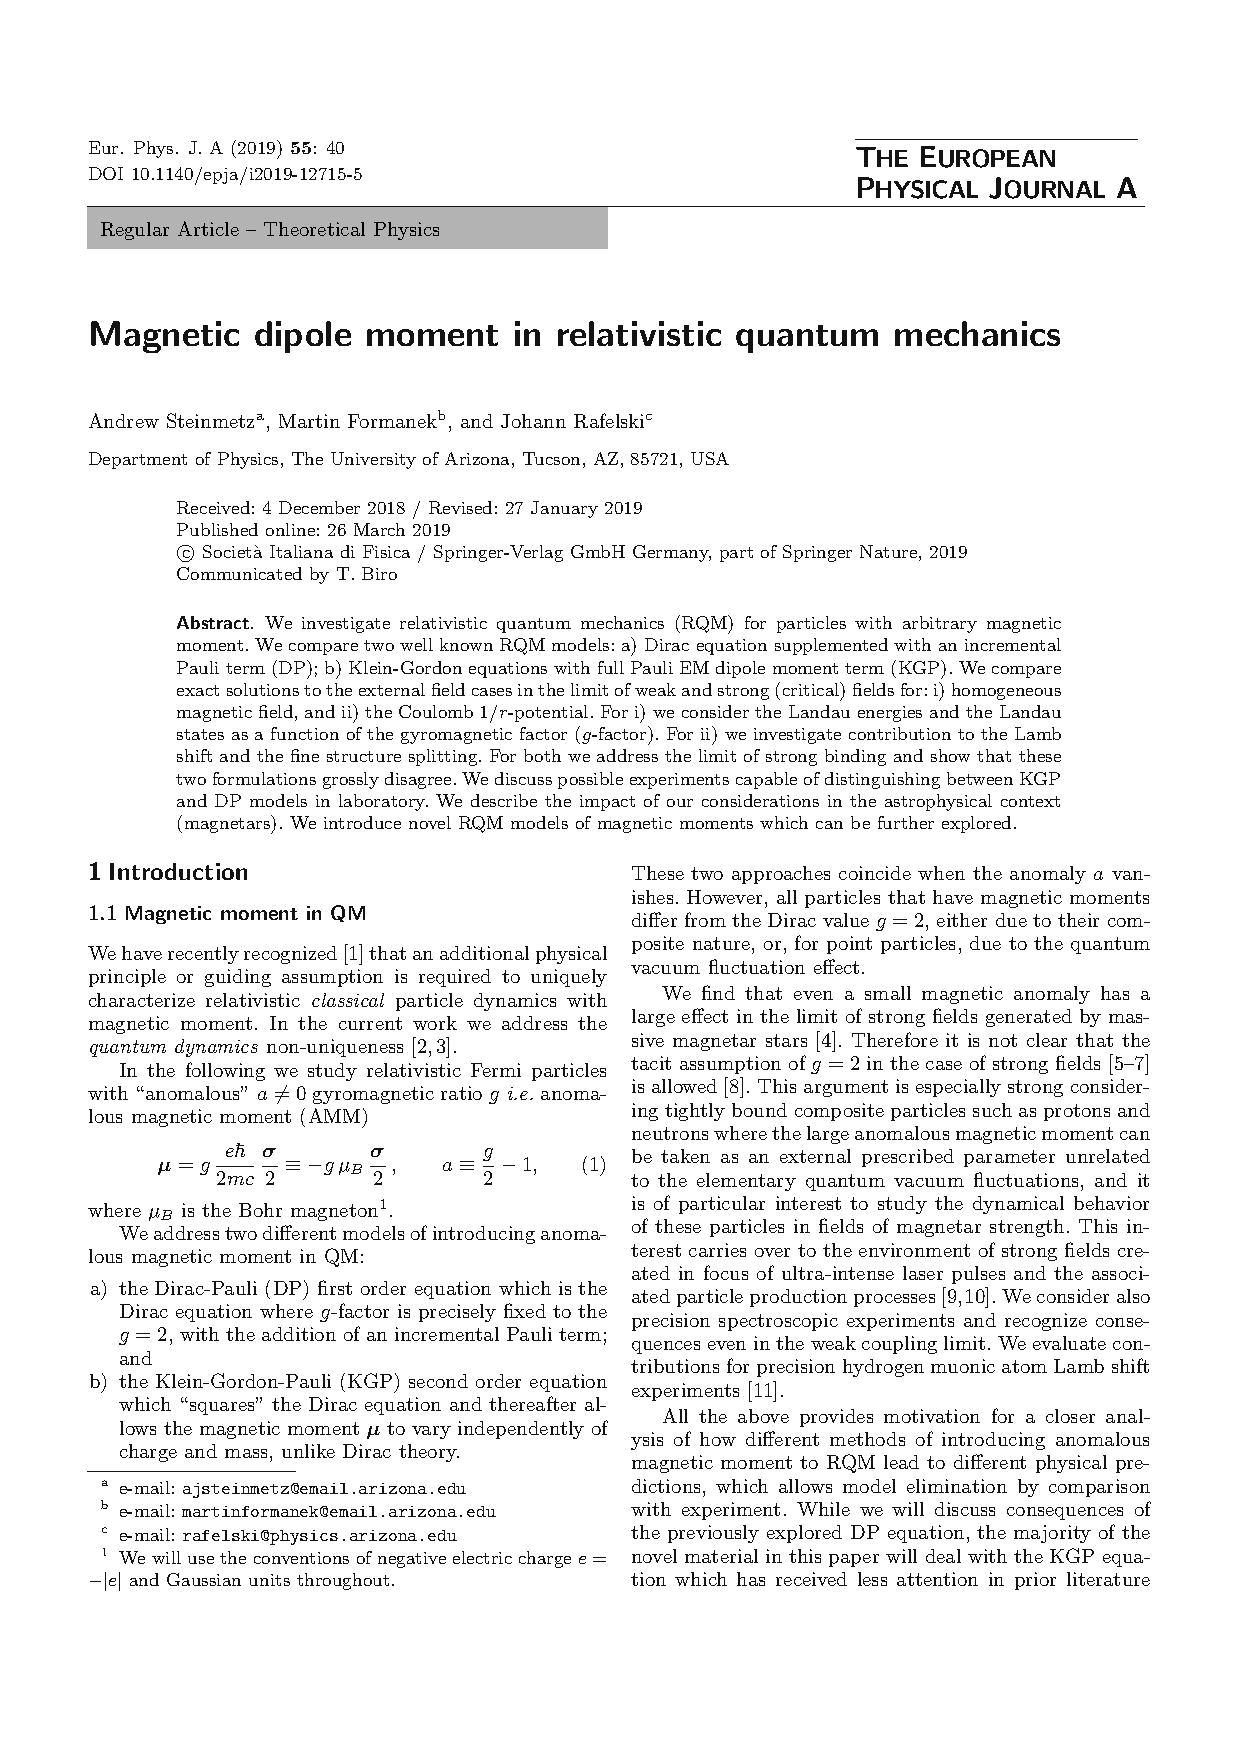
\includepdf[pages=-,pagecommand={},nup=1x2,landscape=true,width=5.5 in]{publications/steinmetz2019magnetic.pdf}

%%%%%%%%%%%%%%%%%%%%%%%%%%%%%%%%%%%%%%%
\chapter{Strong fields and neutral particle magnetic moment dynamics}
\label{appendixB}
%%%%%%%%%%%%%%%%%%%%%%%%%%%%%%%%%%%%%%%
\begin{center}
Formanek, Martin, Stefan Evans, Johann Rafelski, Andrew Steinmetz, and Cheng-Tao Yang. Strong fields and neutral particle magnetic moment dynamics. Plasma Physics and Controlled Fusion 60, 7 (2018): 074006. \href{https://doi.org/10.1088/1361-6587/aac06a}{10.1088/1361-6587/aac06a}
\end{center}

\noindent Copyright (2018) by IOP Publishing. All rights reserved. Reproduced with permission under \href{https://marketplace.copyright.com/rs-ui-web/mp/license/56222509-d3e0-45fd-8ba6-f519e90d4d18/3a89c359-de4e-466f-93c3-ef1135413aab}{License Agreement 1384591-1}. This is the Accepted Manuscript version of an article accepted for publication in Plasma Physics and Controlled Fusion. IOP Publishing Ltd is not responsible for any errors or omissions in this version of the manuscript or any version derived from it. The Version of Record is available online at \href{https://doi.org/10.1088/1361-6587/aac06a}{10.1088/1361-6587/aac06a}.

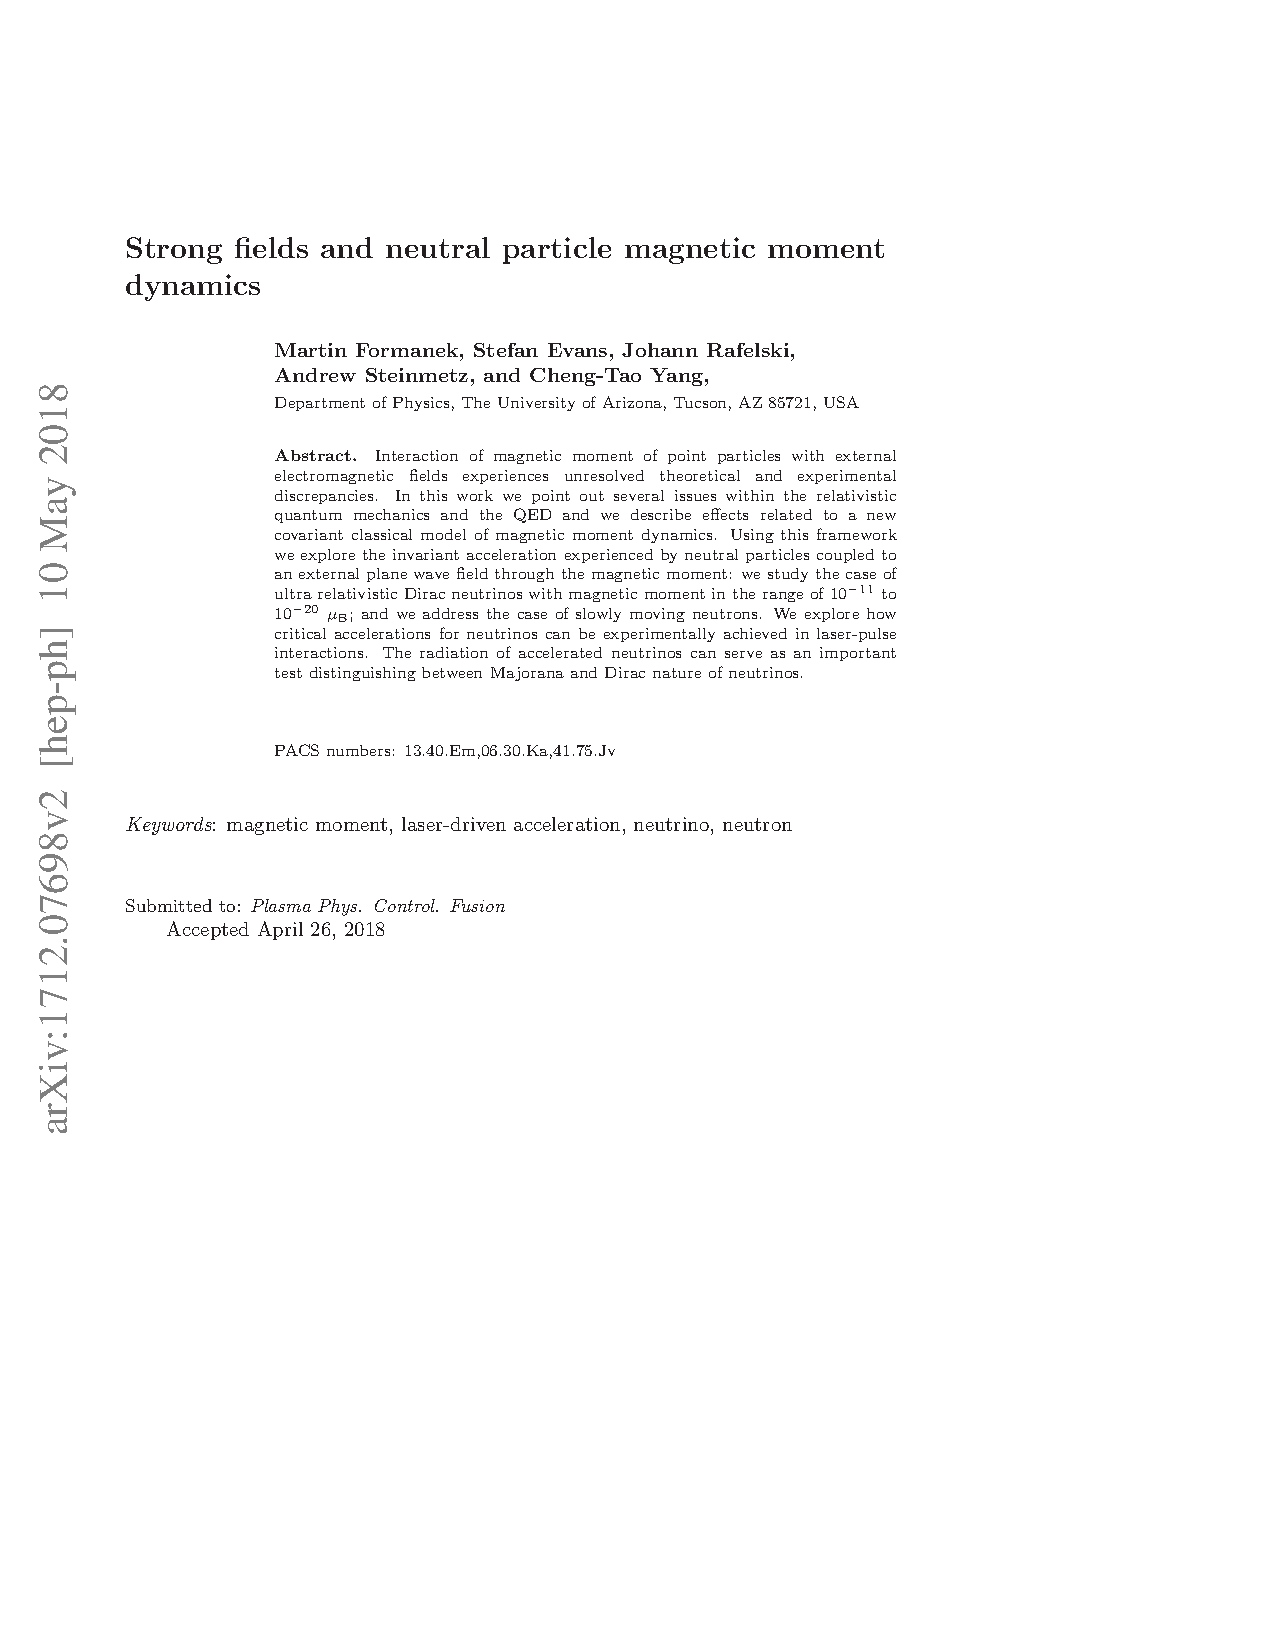
\includepdf[pages=-,pagecommand={},nup=1x2,landscape=true,width=5.5 in]{publications/formanek2018strong.pdf}

%%%%%%%%%%%%%%%%%%%%%%%%%%%%%%%%%%%%%%%
\chapter{Relativistic dynamics of point magnetic moment}
\label{appendixC}
%%%%%%%%%%%%%%%%%%%%%%%%%%%%%%%%%%%%%%%
\begin{center}
Rafelski, J., Formanek, M. \& Steinmetz, A. Relativistic dynamics of point magnetic moment. Eur. Phys. J. C $\bb{78}$, 6 (2018). \href{https://doi.org/10.1140/epjc/s10052-017-5493-2}{10.1140/epjc/s10052-017-5493-2}
\end{center}

\noindent Copyright (2018) by Springer Nature. Reprinted with kind permission of The European Physical Journal (EPJ). This article is an open access article distributed under the terms and conditions of the Creative Commons Attribution \href{https://creativecommons.org/licenses/by/4.0/}{(CC BY 4.0)} license.

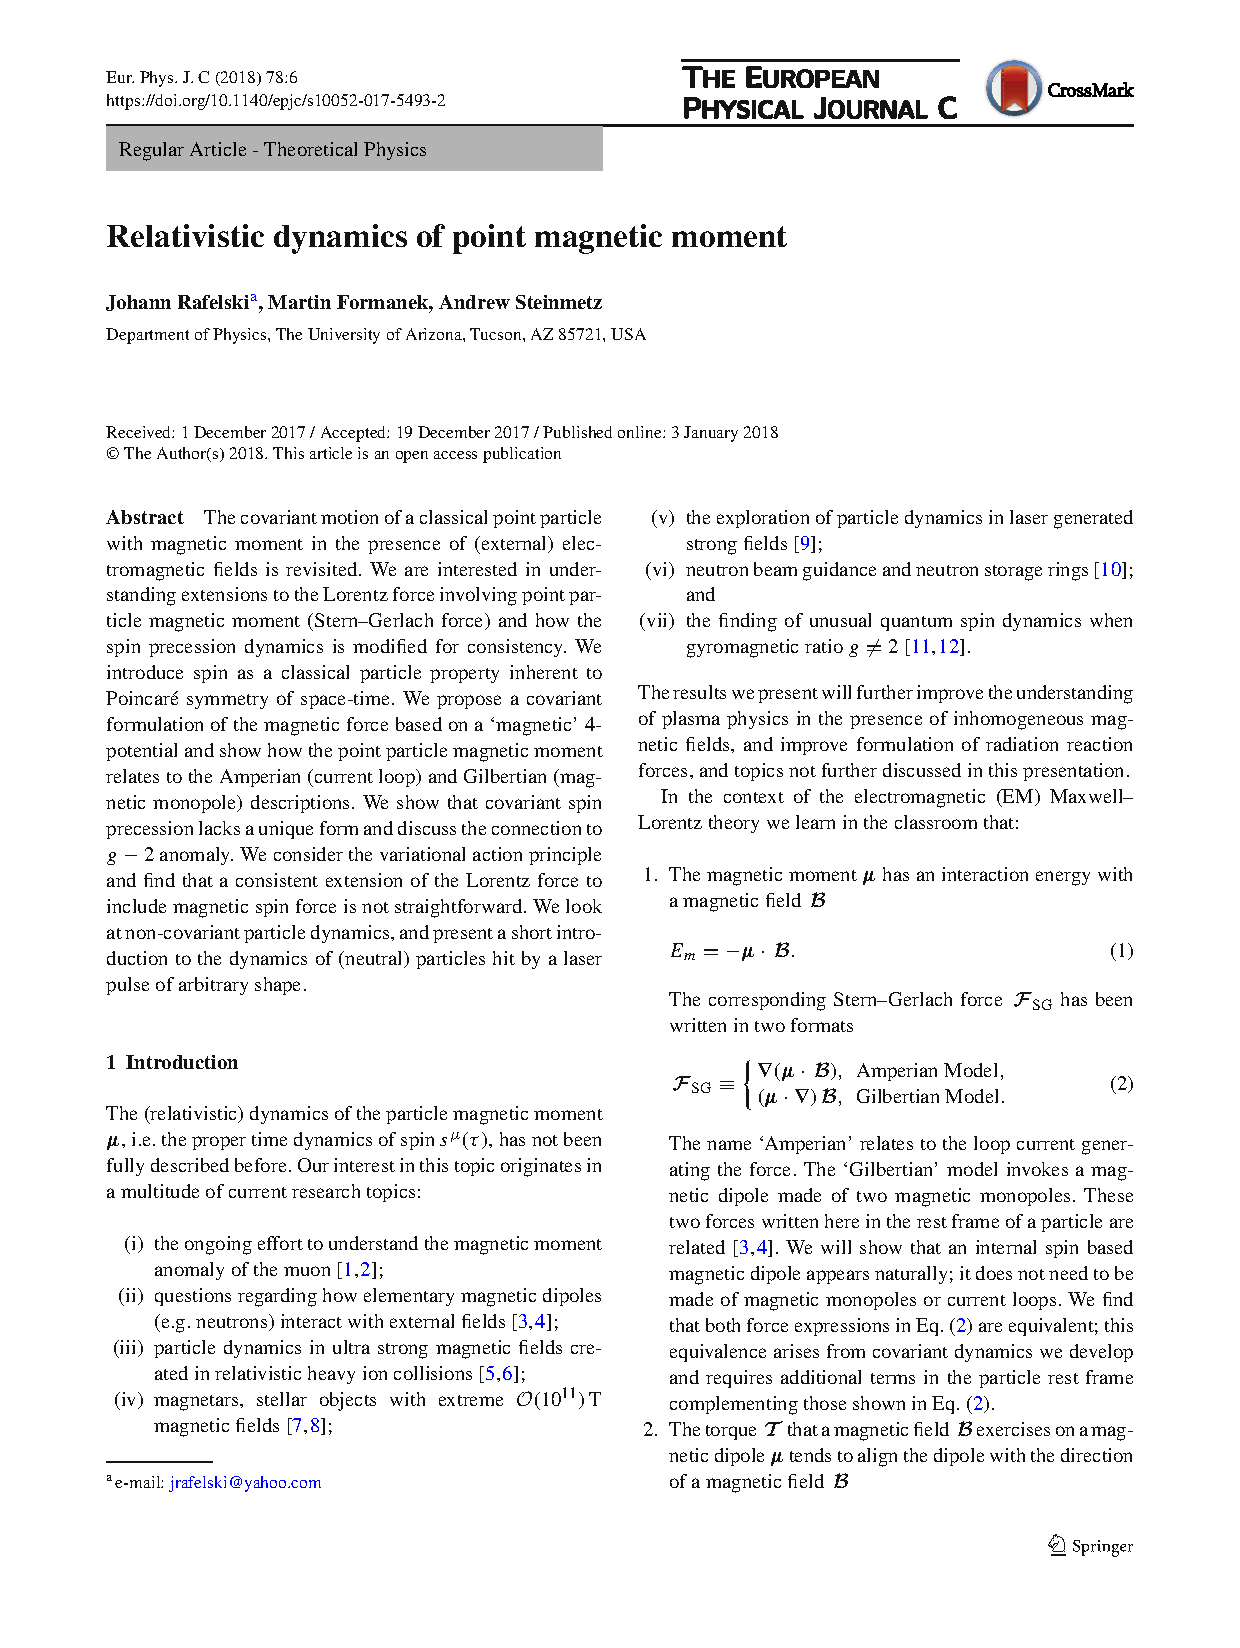
\includepdf[pages=-,pagecommand={},nup=1x2,landscape=true,width=5.5 in]{publications/rafelski2018relativistic.pdf}

%%%%%%%%%%%%%%%%%%%%%%%%%%%%%%%%%%%%%%%
\chapter{A Short Survey of Matter-Antimatter Evolution in the Primordial Universe}
\label{appendixD}
%%%%%%%%%%%%%%%%%%%%%%%%%%%%%%%%%%%%%%%
\begin{center}
Rafelski, J.; Birrell, J.; Steinmetz, A.; Yang, C.T. A Short Survey of Matter-Antimatter Evolution in the Primordial Universe. Universe 2023, 9, 309. \href{https://doi.org/10.3390/universe9070309}{10.3390/universe9070309}
\end{center}

\noindent Copyright (2023) by the authors. Licensee MDPI, Basel, Switzerland. This article is an open access article distributed under the terms and conditions of the Creative Commons Attribution \href{https://creativecommons.org/licenses/by/4.0/}{(CC BY 4.0)} license.

\includepdf[pages=-,pagecommand={},nup=1x2,landscape=true,width=5.5 in]{publications/rafelski2023shortsurvey.pdf}

%%%%%%%%%%%%%%%%%%%%%%%%%%%%%%%%%%%%%%%
\chapter{Antimatter origin of cosmic magnetism: A first look}
\label{appendixE}
%%%%%%%%%%%%%%%%%%%%%%%%%%%%%%%%%%%%%%%
\begin{center}
Steinmetz, A., Yang, C.T. and Rafelski, J. Antimatter origin of cosmic magnetism: A first look. \emph{arXiv preprint}. 2023. XX.XXXXX/arXiv.XXXX.XXXXX
\end{center}

\noindent Copyright (2023) by the authors.

%\includepdf[pages=-,pagecommand={},nup=1x2,landscape=true,width=5.5 in]{publications/rafelski2023shortsurvey.pdf}


\end{document}
